% Options for packages loaded elsewhere
\PassOptionsToPackage{unicode}{hyperref}
\PassOptionsToPackage{hyphens}{url}
%
\documentclass[
]{article}
\usepackage{amsmath,amssymb}
\usepackage{lmodern}
\usepackage{iftex}
\ifPDFTeX
  \usepackage[T1]{fontenc}
  \usepackage[utf8]{inputenc}
  \usepackage{textcomp} % provide euro and other symbols
\else % if luatex or xetex
  \usepackage{unicode-math}
  \defaultfontfeatures{Scale=MatchLowercase}
  \defaultfontfeatures[\rmfamily]{Ligatures=TeX,Scale=1}
\fi
% Use upquote if available, for straight quotes in verbatim environments
\IfFileExists{upquote.sty}{\usepackage{upquote}}{}
\IfFileExists{microtype.sty}{% use microtype if available
  \usepackage[]{microtype}
  \UseMicrotypeSet[protrusion]{basicmath} % disable protrusion for tt fonts
}{}
\makeatletter
\@ifundefined{KOMAClassName}{% if non-KOMA class
  \IfFileExists{parskip.sty}{%
    \usepackage{parskip}
  }{% else
    \setlength{\parindent}{0pt}
    \setlength{\parskip}{6pt plus 2pt minus 1pt}}
}{% if KOMA class
  \KOMAoptions{parskip=half}}
\makeatother
\usepackage{xcolor}
\usepackage[margin=1in]{geometry}
\usepackage{color}
\usepackage{fancyvrb}
\newcommand{\VerbBar}{|}
\newcommand{\VERB}{\Verb[commandchars=\\\{\}]}
\DefineVerbatimEnvironment{Highlighting}{Verbatim}{commandchars=\\\{\}}
% Add ',fontsize=\small' for more characters per line
\usepackage{framed}
\definecolor{shadecolor}{RGB}{248,248,248}
\newenvironment{Shaded}{\begin{snugshade}}{\end{snugshade}}
\newcommand{\AlertTok}[1]{\textcolor[rgb]{0.94,0.16,0.16}{#1}}
\newcommand{\AnnotationTok}[1]{\textcolor[rgb]{0.56,0.35,0.01}{\textbf{\textit{#1}}}}
\newcommand{\AttributeTok}[1]{\textcolor[rgb]{0.77,0.63,0.00}{#1}}
\newcommand{\BaseNTok}[1]{\textcolor[rgb]{0.00,0.00,0.81}{#1}}
\newcommand{\BuiltInTok}[1]{#1}
\newcommand{\CharTok}[1]{\textcolor[rgb]{0.31,0.60,0.02}{#1}}
\newcommand{\CommentTok}[1]{\textcolor[rgb]{0.56,0.35,0.01}{\textit{#1}}}
\newcommand{\CommentVarTok}[1]{\textcolor[rgb]{0.56,0.35,0.01}{\textbf{\textit{#1}}}}
\newcommand{\ConstantTok}[1]{\textcolor[rgb]{0.00,0.00,0.00}{#1}}
\newcommand{\ControlFlowTok}[1]{\textcolor[rgb]{0.13,0.29,0.53}{\textbf{#1}}}
\newcommand{\DataTypeTok}[1]{\textcolor[rgb]{0.13,0.29,0.53}{#1}}
\newcommand{\DecValTok}[1]{\textcolor[rgb]{0.00,0.00,0.81}{#1}}
\newcommand{\DocumentationTok}[1]{\textcolor[rgb]{0.56,0.35,0.01}{\textbf{\textit{#1}}}}
\newcommand{\ErrorTok}[1]{\textcolor[rgb]{0.64,0.00,0.00}{\textbf{#1}}}
\newcommand{\ExtensionTok}[1]{#1}
\newcommand{\FloatTok}[1]{\textcolor[rgb]{0.00,0.00,0.81}{#1}}
\newcommand{\FunctionTok}[1]{\textcolor[rgb]{0.00,0.00,0.00}{#1}}
\newcommand{\ImportTok}[1]{#1}
\newcommand{\InformationTok}[1]{\textcolor[rgb]{0.56,0.35,0.01}{\textbf{\textit{#1}}}}
\newcommand{\KeywordTok}[1]{\textcolor[rgb]{0.13,0.29,0.53}{\textbf{#1}}}
\newcommand{\NormalTok}[1]{#1}
\newcommand{\OperatorTok}[1]{\textcolor[rgb]{0.81,0.36,0.00}{\textbf{#1}}}
\newcommand{\OtherTok}[1]{\textcolor[rgb]{0.56,0.35,0.01}{#1}}
\newcommand{\PreprocessorTok}[1]{\textcolor[rgb]{0.56,0.35,0.01}{\textit{#1}}}
\newcommand{\RegionMarkerTok}[1]{#1}
\newcommand{\SpecialCharTok}[1]{\textcolor[rgb]{0.00,0.00,0.00}{#1}}
\newcommand{\SpecialStringTok}[1]{\textcolor[rgb]{0.31,0.60,0.02}{#1}}
\newcommand{\StringTok}[1]{\textcolor[rgb]{0.31,0.60,0.02}{#1}}
\newcommand{\VariableTok}[1]{\textcolor[rgb]{0.00,0.00,0.00}{#1}}
\newcommand{\VerbatimStringTok}[1]{\textcolor[rgb]{0.31,0.60,0.02}{#1}}
\newcommand{\WarningTok}[1]{\textcolor[rgb]{0.56,0.35,0.01}{\textbf{\textit{#1}}}}
\usepackage{graphicx}
\makeatletter
\def\maxwidth{\ifdim\Gin@nat@width>\linewidth\linewidth\else\Gin@nat@width\fi}
\def\maxheight{\ifdim\Gin@nat@height>\textheight\textheight\else\Gin@nat@height\fi}
\makeatother
% Scale images if necessary, so that they will not overflow the page
% margins by default, and it is still possible to overwrite the defaults
% using explicit options in \includegraphics[width, height, ...]{}
\setkeys{Gin}{width=\maxwidth,height=\maxheight,keepaspectratio}
% Set default figure placement to htbp
\makeatletter
\def\fps@figure{htbp}
\makeatother
\setlength{\emergencystretch}{3em} % prevent overfull lines
\providecommand{\tightlist}{%
  \setlength{\itemsep}{0pt}\setlength{\parskip}{0pt}}
\setcounter{secnumdepth}{-\maxdimen} % remove section numbering
\ifLuaTeX
  \usepackage{selnolig}  % disable illegal ligatures
\fi
\IfFileExists{bookmark.sty}{\usepackage{bookmark}}{\usepackage{hyperref}}
\IfFileExists{xurl.sty}{\usepackage{xurl}}{} % add URL line breaks if available
\urlstyle{same} % disable monospaced font for URLs
\hypersetup{
  pdftitle={Practica1},
  hidelinks,
  pdfcreator={LaTeX via pandoc}}

\title{Practica1}
\author{}
\date{\vspace{-2.5em}2022-08-29}

\begin{document}
\maketitle

\#Ejericio 1:

Cargamos los datos Debernardi.csv

\begin{Shaded}
\begin{Highlighting}[]
\FunctionTok{setwd}\NormalTok{(}\StringTok{"\textasciitilde{}/Documents/FCEyN/Estadistica/Datos"}\NormalTok{)}
\NormalTok{debD }\OtherTok{=} \FunctionTok{read.csv}\NormalTok{(}\StringTok{"Debernardi.csv"}\NormalTok{)}
\NormalTok{debD}
\end{Highlighting}
\end{Shaded}

\begin{verbatim}
##     sample_id patient_cohort sample_origin age sex diagnosis stage
## 1          S1        Cohort1          BPTB  33   F         1      
## 2         S10        Cohort1          BPTB  81   F         1      
## 3        S100        Cohort2          BPTB  51   M         1      
## 4        S101        Cohort2          BPTB  61   M         1      
## 5        S102        Cohort2          BPTB  62   M         1      
## 6        S103        Cohort2          BPTB  53   M         1      
## 7        S104        Cohort2          BPTB  70   M         1      
## 8        S105        Cohort2          BPTB  58   F         1      
## 9        S106        Cohort2          BPTB  59   F         1      
## 10       S107        Cohort2          BPTB  56   F         1      
## 11       S108        Cohort2          BPTB  77   F         1      
## 12       S109        Cohort2          BPTB  71   M         1      
## 13        S11        Cohort1          BPTB  49   F         1      
## 14       S110        Cohort2          BPTB  53   M         1      
## 15       S111        Cohort2          BPTB  56   F         1      
## 16       S112        Cohort2          BPTB  60   F         1      
## 17       S113        Cohort2          BPTB  69   F         1      
## 18       S114        Cohort2          BPTB  60   F         1      
## 19       S115        Cohort2          BPTB  55   M         1      
## 20       S116        Cohort1          BPTB  28   F         1      
## 21       S117        Cohort1          BPTB  54   F         1      
## 22       S118        Cohort1          BPTB  50   F         1      
## 23       S119        Cohort1          BPTB  40   M         1      
## 24        S12        Cohort1          BPTB  74   F         1      
## 25       S120        Cohort1          BPTB  63   M         1      
## 26       S121        Cohort1          BPTB  50   M         1      
## 27       S122        Cohort1          BPTB  47   M         1      
## 28       S123        Cohort1          BPTB  45   M         1      
## 29       S124        Cohort1          BPTB  35   M         1      
## 30       S125        Cohort1          BPTB  30   M         1      
## 31       S126        Cohort2          BPTB  48   F         1      
## 32       S127        Cohort2          BPTB  44   F         1      
## 33       S128        Cohort2          BPTB  44   F         1      
## 34       S129        Cohort2          BPTB  56   F         1      
## 35        S13        Cohort1          BPTB  58   F         1      
## 36       S130        Cohort2          BPTB  44   F         1      
## 37       S131        Cohort2          BPTB  48   F         1      
## 38       S132        Cohort2          BPTB  48   F         1      
## 39       S133        Cohort2          BPTB  41   F         1      
## 40       S134        Cohort2          BPTB  45   F         1      
## 41       S135        Cohort2          BPTB  45   F         1      
## 42       S136        Cohort2          BPTB  45   F         1      
## 43       S137        Cohort2          BPTB  48   F         1      
## 44       S138        Cohort2          BPTB  89   F         1      
## 45       S139        Cohort2          BPTB  87   M         1      
## 46        S14        Cohort1          BPTB  50   F         1      
## 47       S140        Cohort2          BPTB  66   F         1      
## 48       S141        Cohort2          BPTB  59   M         1      
## 49       S142        Cohort2          BPTB  59   M         1      
## 50       S143        Cohort2          BPTB  36   F         1      
## 51       S144        Cohort2          BPTB  70   F         1      
## 52       S145        Cohort2          BPTB  63   F         1      
## 53       S146        Cohort2          BPTB  63   F         1      
## 54       S147        Cohort2          BPTB  59   M         1      
## 55       S148        Cohort2          BPTB  67   F         1      
## 56       S149        Cohort2          BPTB  49   M         1      
## 57        S15        Cohort1          BPTB  87   F         1      
## 58       S150        Cohort2          BPTB  47   M         1      
## 59       S151        Cohort2          BPTB  60   F         1      
## 60       S152        Cohort2          BPTB  60   F         1      
## 61       S153        Cohort2          BPTB  73   F         1      
## 62       S154        Cohort2          BPTB  83   F         1      
## 63       S155        Cohort2          BPTB  60   F         1      
## 64       S156        Cohort2          BPTB  44   F         1      
## 65       S157        Cohort2          BPTB  55   F         1      
## 66       S158        Cohort2          BPTB  51   F         1      
## 67       S159        Cohort2          BPTB  56   F         1      
## 68        S16        Cohort1          BPTB  60   M         1      
## 69       S160        Cohort2          BPTB  65   F         1      
## 70       S161        Cohort2          BPTB  45   M         1      
## 71       S162        Cohort2          BPTB  64   F         1      
## 72       S163        Cohort2          BPTB  26   F         1      
## 73       S164        Cohort2          BPTB  34   F         1      
## 74       S165        Cohort2          BPTB  45   F         1      
## 75       S166        Cohort2          BPTB  51   F         1      
## 76       S167        Cohort2          BPTB  67   F         1      
## 77       S168        Cohort2          BPTB  64   F         1      
## 78       S169        Cohort2          BPTB  50   F         1      
## 79        S17        Cohort1          BPTB  49   M         1      
## 80       S170        Cohort2          BPTB  63   F         1      
## 81       S171        Cohort2          BPTB  81   F         1      
## 82       S172        Cohort2          BPTB  71   M         1      
## 83       S173        Cohort2          BPTB  71   F         1      
## 84       S174        Cohort2          BPTB  35   F         1      
## 85       S175        Cohort2          BPTB  57   F         1      
## 86       S176        Cohort2          BPTB  64   M         1      
## 87       S177        Cohort2          BPTB  40   M         1      
## 88       S178        Cohort2          BPTB  46   M         1      
## 89       S179        Cohort2          BPTB  61   F         1      
## 90        S18        Cohort1          BPTB  58   F         1      
## 91       S180        Cohort2          BPTB  71   F         1      
## 92       S181        Cohort2          BPTB  38   F         1      
## 93       S182        Cohort2          BPTB  50   M         1      
## 94       S183        Cohort2          BPTB  84   F         1      
## 95        S19        Cohort1          BPTB  63   F         1      
## 96         S2        Cohort1          BPTB  69   F         1      
## 97        S20        Cohort1          BPTB  74   F         1      
## 98        S21        Cohort1          BPTB  64   M         1      
## 99        S22        Cohort1          BPTB  68   F         1      
## 100       S23        Cohort2          BPTB  50   F         1      
## 101       S24        Cohort1          BPTB  56   F         1      
## 102       S25        Cohort1          BPTB  50   F         1      
## 103       S26        Cohort1          BPTB  51   M         1      
## 104       S27        Cohort1          BPTB  44   F         1      
## 105       S28        Cohort1          BPTB  74   M         1      
## 106       S29        Cohort1          BPTB  49   M         1      
## 107        S3        Cohort2          BPTB  49   F         1      
## 108       S30        Cohort1          BPTB  58   F         1      
## 109       S31        Cohort1          BPTB  49   M         1      
## 110       S32        Cohort1          BPTB  55   M         1      
## 111       S33        Cohort1          BPTB  50   M         1      
## 112       S34        Cohort1          BPTB  46   M         1      
## 113       S35        Cohort1          BPTB  61   F         1      
## 114       S36        Cohort1          BPTB  48   F         1      
## 115       S37        Cohort1          BPTB  58   M         1      
## 116       S38        Cohort1          BPTB  47   M         1      
## 117       S39        Cohort1          BPTB  51   M         1      
## 118        S4        Cohort2          BPTB  37   M         1      
## 119       S40        Cohort1          BPTB  57   M         1      
## 120       S41        Cohort1          BPTB  46   M         1      
## 121       S42        Cohort1          BPTB  62   M         1      
## 122       S43        Cohort1          BPTB  64   M         1      
## 123       S44        Cohort1          BPTB  49   M         1      
## 124       S45        Cohort1          BPTB  52   M         1      
## 125       S46        Cohort1          BPTB  57   F         1      
## 126       S47        Cohort1          BPTB  61   F         1      
## 127       S48        Cohort1          BPTB  40   M         1      
## 128       S49        Cohort1          BPTB  58   F         1      
## 129        S5        Cohort1          BPTB  78   M         1      
## 130       S50        Cohort1          BPTB  53   M         1      
## 131       S51        Cohort1          BPTB  56   M         1      
## 132       S52        Cohort1          BPTB  56   M         1      
## 133       S53        Cohort1          BPTB  54   M         1      
## 134       S54        Cohort1          BPTB  62   M         1      
## 135       S55        Cohort1          BPTB  61   M         1      
## 136       S56        Cohort1          BPTB  67   F         1      
## 137       S57        Cohort1          BPTB  40   F         1      
## 138       S58        Cohort1          BPTB  56   F         1      
## 139       S59        Cohort1          BPTB  47   M         1      
## 140        S6        Cohort1          BPTB  73   F         1      
## 141       S60        Cohort1          BPTB  55   M         1      
## 142       S61        Cohort1          BPTB  62   F         1      
## 143       S62        Cohort2          BPTB  43   F         1      
## 144       S63        Cohort1          BPTB  76   F         1      
## 145       S64        Cohort1          BPTB  48   F         1      
## 146       S65        Cohort2          BPTB  41   F         1      
## 147       S66        Cohort1          BPTB  62   F         1      
## 148       S67        Cohort1          BPTB  71   M         1      
## 149       S68        Cohort1          BPTB  54   F         1      
## 150       S69        Cohort1          BPTB  52   F         1      
## 151        S7        Cohort1          BPTB  56   F         1      
## 152       S70        Cohort1          BPTB  57   M         1      
## 153       S71        Cohort1          BPTB  58   F         1      
## 154       S72        Cohort1          BPTB  58   F         1      
## 155       S73        Cohort1          BPTB  62   F         1      
## 156       S74        Cohort2          BPTB  69   F         1      
## 157       S75        Cohort1          BPTB  28   F         1      
## 158       S76        Cohort1          BPTB  30   F         1      
## 159       S77        Cohort1          BPTB  41   F         1      
## 160       S78        Cohort2          BPTB  43   M         1      
## 161       S79        Cohort2          BPTB  30   F         1      
## 162        S8        Cohort1          BPTB  61   M         1      
## 163       S80        Cohort2          BPTB  58   M         1      
## 164       S81        Cohort2          BPTB  50   M         1      
## 165       S82        Cohort2          BPTB  55   M         1      
## 166       S83        Cohort2          BPTB  59   F         1      
## 167       S84        Cohort2          BPTB  66   F         1      
## 168       S85        Cohort2          BPTB  62   F         1      
## 169       S86        Cohort2          BPTB  72   F         1      
## 170       S87        Cohort2          BPTB  63   M         1      
## 171       S88        Cohort2          BPTB  65   M         1      
## 172       S89        Cohort2          BPTB  68   F         1      
## 173        S9        Cohort1          BPTB  57   M         1      
## 174       S90        Cohort2          BPTB  59   M         1      
## 175       S91        Cohort2          BPTB  53   F         1      
## 176       S92        Cohort2          BPTB  73   F         1      
## 177       S93        Cohort2          BPTB  54   F         1      
## 178       S94        Cohort2          BPTB  63   F         1      
## 179       S95        Cohort2          BPTB  66   F         1      
## 180       S96        Cohort2          BPTB  65   F         1      
## 181       S97        Cohort2          BPTB  69   F         1      
## 182       S98        Cohort2          BPTB  62   F         1      
## 183       S99        Cohort2          BPTB  76   F         1      
## 184      S271        Cohort2          BPTB  32   F         2      
## 185      S299        Cohort2          BPTB  59   F         2      
## 186      S308        Cohort2          BPTB  65   F         2      
## 187      S314        Cohort2          BPTB  39   F         2      
## 188      S315        Cohort2          BPTB  65   F         2      
## 189      S344        Cohort2          BPTB  59   M         2      
## 190      S338        Cohort1          BPTB  52   M         2      
## 191      S329        Cohort2          BPTB  61   F         2      
## 192      S260        Cohort2          BPTB  55   F         2      
## 193      S261        Cohort2          BPTB  74   F         2      
## 194      S263        Cohort2          BPTB  71   F         2      
## 195      S274        Cohort2          BPTB  52   F         2      
## 196      S275        Cohort2          BPTB  37   F         2      
## 197      S280        Cohort2          BPTB  41   F         2      
## 198      S282        Cohort2          BPTB  60   F         2      
## 199      S321        Cohort2          BPTB  46   M         2      
## 200      S323        Cohort2          BPTB  29   F         2      
## 201      S363        Cohort2          BPTB  60   F         2      
## 202      S365        Cohort2          BPTB  26   F         2      
## 203      S371        Cohort2          BPTB  52   F         2      
## 204      S361        Cohort2          BPTB  78   M         2      
## 205      S362        Cohort2          BPTB  28   F         2      
## 206      S364        Cohort2          BPTB  50   F         2      
## 207      S272        Cohort2          BPTB  38   F         2      
## 208      S246        Cohort2          BPTB  68   M         2      
## 209      S257        Cohort2          BPTB  36   F         2      
## 210      S316        Cohort2          BPTB  54   M         2      
## 211      S347        Cohort2          BPTB  73   M         2      
## 212      S350        Cohort2          BPTB  82   F         2      
## 213      S368        Cohort1          BPTB  68   F         2      
## 214      S278        Cohort2          BPTB  72   F         2      
## 215      S320        Cohort2          BPTB  54   F         2      
## 216      S369        Cohort1          BPTB  53   M         2      
## 217      S370        Cohort2          BPTB  62   M         2      
## 218      S279        Cohort2          BPTB  36   F         2      
## 219      S298        Cohort2          BPTB  31   M         2      
## 220      S296        Cohort2          BPTB  68   M         2      
## 221      S290        Cohort2          BPTB  54   M         2      
## 222      S292        Cohort2          BPTB  43   F         2      
## 223      S293        Cohort2          BPTB  56   F         2      
## 224      S306        Cohort2          BPTB  75   M         2      
## 225      S309        Cohort2          BPTB  55   F         2      
## 226      S310        Cohort2          BPTB  41   M         2      
## 227      S311        Cohort2          BPTB  40   F         2      
## 228      S312        Cohort2          BPTB  46   F         2      
## 229      S313        Cohort2          BPTB  37   F         2      
## 230      S327        Cohort2          BPTB  41   M         2      
## 231      S328        Cohort2          BPTB  62   M         2      
## 232      S333        Cohort2          BPTB  40   M         2      
## 233      S336        Cohort2          BPTB  49   F         2      
## 234      S339        Cohort2          BPTB  68   M         2      
## 235      S341        Cohort2          BPTB  69   F         2      
## 236      S342        Cohort2          BPTB  65   M         2      
## 237      S343        Cohort2          BPTB  66   F         2      
## 238      S348        Cohort1          BPTB  63   M         2      
## 239      S353        Cohort2          BPTB  48   M         2      
## 240      S354        Cohort2          BPTB  41   M         2      
## 241      S355        Cohort2          BPTB  38   F         2      
## 242      S250        Cohort2          BPTB  65   F         2      
## 243      S269        Cohort2          BPTB  49   F         2      
## 244      S346        Cohort2          BPTB  75   M         2      
## 245      S351        Cohort2          BPTB  52   F         2      
## 246      S352        Cohort2          BPTB  53   F         2      
## 247      S245        Cohort2          BPTB  53   M         2      
## 248      S357        Cohort2          BPTB  40   M         2      
## 249      S273        Cohort2          BPTB  77   F         2      
## 250      S265        Cohort2          BPTB  70   F         2      
## 251      S331        Cohort2          BPTB  79   M         2      
## 252      S184        Cohort1           LIV  39   F         2      
## 253      S185        Cohort1           LIV  38   F         2      
## 254      S186        Cohort1           LIV  31   M         2      
## 255      S187        Cohort1           LIV  73   F         2      
## 256      S188        Cohort1           LIV  59   M         2      
## 257      S189        Cohort1           LIV  44   M         2      
## 258      S190        Cohort1           LIV  67   M         2      
## 259      S191        Cohort1           LIV  55   M         2      
## 260      S192        Cohort1           LIV  37   F         2      
## 261      S193        Cohort1           LIV  42   M         2      
## 262      S194        Cohort1           LIV  38   M         2      
## 263      S195        Cohort1           LIV  71   M         2      
## 264      S196        Cohort1           LIV  50   F         2      
## 265      S197        Cohort1           LIV  35   M         2      
## 266      S198        Cohort1           LIV  39   F         2      
## 267      S199        Cohort1           LIV  48   F         2      
## 268      S200        Cohort1           LIV  66   M         2      
## 269      S201        Cohort1           LIV  51   F         2      
## 270      S202        Cohort1           LIV  42   M         2      
## 271      S203        Cohort1           LIV  50   M         2      
## 272      S204        Cohort1           LIV  70   F         2      
## 273      S205        Cohort1           LIV  31   M         2      
## 274      S206        Cohort1           LIV  68   F         2      
## 275      S207        Cohort1           LIV  64   M         2      
## 276      S208        Cohort1           LIV  64   M         2      
## 277      S209        Cohort1           LIV  60   F         2      
## 278      S210        Cohort1           LIV  67   M         2      
## 279      S211        Cohort1           LIV  44   M         2      
## 280      S212        Cohort1           LIV  53   F         2      
## 281      S213        Cohort1           LIV  49   F         2      
## 282      S214        Cohort1           LIV  72   M         2      
## 283      S215        Cohort1           LIV  57   F         2      
## 284      S216        Cohort1           LIV  66   M         2      
## 285      S217        Cohort1           LIV  47   M         2      
## 286      S218        Cohort1           LIV  70   M         2      
## 287      S219        Cohort1           LIV  40   F         2      
## 288      S220        Cohort1           LIV  53   F         2      
## 289      S221        Cohort1           LIV  73   M         2      
## 290      S222        Cohort1           LIV  44   M         2      
## 291      S285        Cohort2          BPTB  52   F         2      
## 292      S340        Cohort2          BPTB  45   M         2      
## 293      S356        Cohort1          BPTB  64   F         2      
## 294      S303        Cohort2          BPTB  52   F         2      
## 295      S319        Cohort2          BPTB  29   F         2      
## 296      S229        Cohort1          BPTB  46   F         2      
## 297      S233        Cohort1          BPTB  46   M         2      
## 298      S238        Cohort2          BPTB  42   M         2      
## 299      S295        Cohort2          BPTB  45   M         2      
## 300      S234        Cohort2          BPTB  40   F         2      
## 301      S251        Cohort2          BPTB  40   M         2      
## 302      S252        Cohort1          BPTB  48   M         2      
## 303      S256        Cohort2          BPTB  57   F         2      
## 304      S262        Cohort2          BPTB  69   M         2      
## 305      S264        Cohort1          BPTB  57   M         2      
## 306      S267        Cohort2          BPTB  47   M         2      
## 307      S281        Cohort1          BPTB  62   M         2      
## 308      S325        Cohort2          BPTB  42   M         2      
## 309      S349        Cohort1          BPTB  41   M         2      
## 310      S358        Cohort2          BPTB  57   M         2      
## 311      S249        Cohort1          BPTB  51   M         2      
## 312      S243        Cohort2          BPTB  65   M         2      
## 313      S244        Cohort1          BPTB  67   M         2      
## 314      S284        Cohort2          BPTB  78   M         2      
## 315      S242        Cohort2          BPTB  61   F         2      
## 316      S334        Cohort2          BPTB  54   M         2      
## 317      S223        Cohort1           ESP  68   F         2      
## 318      S224        Cohort1           ESP  54   F         2      
## 319      S225        Cohort1           ESP  54   M         2      
## 320      S226        Cohort1           ESP  58   M         2      
## 321      S227        Cohort1           ESP  66   M         2      
## 322      S228        Cohort1           ESP  55   M         2      
## 323      S230        Cohort1          BPTB  48   M         2      
## 324      S232        Cohort2          BPTB  66   M         2      
## 325      S241        Cohort2          BPTB  69   F         2      
## 326      S258        Cohort2          BPTB  55   F         2      
## 327      S286        Cohort1          BPTB  56   M         2      
## 328      S304        Cohort2          BPTB  58   M         2      
## 329      S307        Cohort1          BPTB  67   F         2      
## 330      S318        Cohort1          BPTB  47   M         2      
## 331      S366        Cohort1          BPTB  54   F         2      
## 332      S372        Cohort1           UCL  43   M         2      
## 333      S373        Cohort1           UCL  53   F         2      
## 334      S374        Cohort1           UCL  30   F         2      
## 335      S375        Cohort1           UCL  48   F         2      
## 336      S376        Cohort1           UCL  71   M         2      
## 337      S377        Cohort1           UCL  53   M         2      
## 338      S378        Cohort1           UCL  36   F         2      
## 339      S379        Cohort1           UCL  60   M         2      
## 340      S380        Cohort1           UCL  70   F         2      
## 341      S381        Cohort1           UCL  80   M         2      
## 342      S382        Cohort1           UCL  74   F         2      
## 343      S383        Cohort1           UCL  45   F         2      
## 344      S384        Cohort1           UCL  43   M         2      
## 345      S385        Cohort1           UCL  50   M         2      
## 346      S386        Cohort1           UCL  68   M         2      
## 347      S387        Cohort1           UCL  82   M         2      
## 348      S388        Cohort1           UCL  75   M         2      
## 349      S389        Cohort1           UCL  61   M         2      
## 350      S390        Cohort1           UCL  67   M         2      
## 351      S391        Cohort1           UCL  32   M         2      
## 352      S367        Cohort1          BPTB  46   M         2      
## 353      S231        Cohort1          BPTB  71   M         2      
## 354      S322        Cohort2          BPTB  42   M         2      
## 355      S305        Cohort2          BPTB  56   M         2      
## 356      S237        Cohort2          BPTB  46   M         2      
## 357      S240        Cohort2          BPTB  52   F         2      
## 358      S317        Cohort2          BPTB  80   M         2      
## 359      S345        Cohort2          BPTB  70   M         2      
## 360      S294        Cohort1          BPTB  40   M         2      
## 361      S239        Cohort1          BPTB  29   M         2      
## 362      S326        Cohort2          BPTB  58   M         2      
## 363      S248        Cohort2          BPTB  48   M         2      
## 364      S253        Cohort2          BPTB  66   F         2      
## 365      S254        Cohort1          BPTB  74   F         2      
## 366      S324        Cohort2          BPTB  41   F         2      
## 367      S291        Cohort2          BPTB  53   M         2      
## 368      S301        Cohort2          BPTB  38   F         2      
## 369      S332        Cohort2          BPTB  29   M         2      
## 370      S337        Cohort1          BPTB  55   M         2      
## 371      S287        Cohort2          BPTB  58   F         2      
## 372      S297        Cohort2          BPTB  77   F         2      
## 373      S277        Cohort2          BPTB  67   F         2      
## 374      S268        Cohort2          BPTB  47   F         2      
## 375      S270        Cohort2          BPTB  50   F         2      
## 376      S359        Cohort2          BPTB  44   F         2      
## 377      S255        Cohort2          BPTB  66   M         2      
## 378      S289        Cohort2          BPTB  52   M         2      
## 379      S235        Cohort2          BPTB  72   M         2      
## 380      S276        Cohort2          BPTB  59   F         2      
## 381      S236        Cohort2          BPTB  76   F         2      
## 382      S247        Cohort2          BPTB  40   F         2      
## 383      S266        Cohort2          BPTB  47   F         2      
## 384      S283        Cohort2          BPTB  64   F         2      
## 385      S330        Cohort2          BPTB  46   F         2      
## 386      S335        Cohort2          BPTB  75   F         2      
## 387      S360        Cohort2          BPTB  49   F         2      
## 388      S259        Cohort2          BPTB  53   F         2      
## 389      S300        Cohort2          BPTB  74   F         2      
## 390      S302        Cohort2          BPTB  69   M         2      
## 391      S288        Cohort2          BPTB  63   F         2      
## 392      S497        Cohort1           ESP  81   F         3     I
## 393      S456        Cohort1           LIV  57   M         3    IA
## 394      S520        Cohort1          BPTB  55   M         3    IA
## 395      S573        Cohort2          BPTB  58   M         3    IA
## 396      S401        Cohort1           LIV  73   M         3    IB
## 397      S410        Cohort1           LIV  75   M         3    IB
## 398      S482        Cohort1          BPTB  68   F         3    IB
## 399      S531        Cohort1          BPTB  77   F         3    IB
## 400      S534        Cohort1          BPTB  56   M         3    IB
## 401      S577        Cohort2          BPTB  67   M         3    IB
## 402      S584        Cohort2           LIV  75   M         3    IB
## 403      S585        Cohort2           LIV  74   F         3    IB
## 404      S586        Cohort2           LIV  77   M         3    IB
## 405      S587        Cohort2           LIV  63   F         3    IB
## 406      S588        Cohort2           LIV  60   F         3    IB
## 407      S589        Cohort2           LIV  52   F         3    IB
## 408      S496        Cohort1           ESP  69   F         3    II
## 409      S498        Cohort1           ESP  53   M         3    II
## 410      S502        Cohort1           ESP  82   F         3    II
## 411      S504        Cohort1           ESP  54   M         3    II
## 412      S508        Cohort1           ESP  66   M         3    II
## 413      S517        Cohort1           ESP  81   F         3    II
## 414      S518        Cohort1           ESP  55   M         3    II
## 415      S419        Cohort1           LIV  68   M         3   IIA
## 416      S426        Cohort1           LIV  67   M         3   IIA
## 417      S427        Cohort1           LIV  75   F         3   IIA
## 418      S437        Cohort1           LIV  64   F         3   IIA
## 419      S438        Cohort1           LIV  64   F         3   IIA
## 420      S441        Cohort1           LIV  55   M         3   IIA
## 421      S444        Cohort1           LIV  56   F         3   IIA
## 422      S451        Cohort1           LIV  72   M         3   IIA
## 423      S527        Cohort2          BPTB  48   M         3   IIA
## 424      S530        Cohort1          BPTB  73   F         3   IIA
## 425      S553        Cohort2          BPTB  71   F         3   IIA
## 426      S394        Cohort1           LIV  73   M         3   IIB
## 427      S396        Cohort1           LIV  62   F         3   IIB
## 428      S399        Cohort1           LIV  69   M         3   IIB
## 429      S403        Cohort1           LIV  66   M         3   IIB
## 430      S404        Cohort1           LIV  74   F         3   IIB
## 431      S407        Cohort1           LIV  77   M         3   IIB
## 432      S411        Cohort1           LIV  77   M         3   IIB
## 433      S413        Cohort1           LIV  61   M         3   IIB
## 434      S414        Cohort1           LIV  58   F         3   IIB
## 435      S415        Cohort1           LIV  69   F         3   IIB
## 436      S416        Cohort1           LIV  61   F         3   IIB
## 437      S418        Cohort1           LIV  77   M         3   IIB
## 438      S420        Cohort1           LIV  62   M         3   IIB
## 439      S421        Cohort1           LIV  45   F         3   IIB
## 440      S422        Cohort1           LIV  67   F         3   IIB
## 441      S423        Cohort1           LIV  68   M         3   IIB
## 442      S425        Cohort1           LIV  71   M         3   IIB
## 443      S429        Cohort1           LIV  75   F         3   IIB
## 444      S431        Cohort1           LIV  63   F         3   IIB
## 445      S432        Cohort1           LIV  71   M         3   IIB
## 446      S433        Cohort1           LIV  73   M         3   IIB
## 447      S440        Cohort1           LIV  54   F         3   IIB
## 448      S442        Cohort1           LIV  59   F         3   IIB
## 449      S443        Cohort1           LIV  61   F         3   IIB
## 450      S447        Cohort1           LIV  74   F         3   IIB
## 451      S448        Cohort1           LIV  73   F         3   IIB
## 452      S449        Cohort1           LIV  78   F         3   IIB
## 453      S450        Cohort1           LIV  70   M         3   IIB
## 454      S452        Cohort1           LIV  82   F         3   IIB
## 455      S453        Cohort1           LIV  58   M         3   IIB
## 456      S454        Cohort1           LIV  62   M         3   IIB
## 457      S455        Cohort1           LIV  76   F         3   IIB
## 458      S461        Cohort1           LIV  79   F         3   IIB
## 459      S465        Cohort1           LIV  68   M         3   IIB
## 460      S466        Cohort1           LIV  70   M         3   IIB
## 461      S471        Cohort1           LIV  62   F         3   IIB
## 462      S472        Cohort1           LIV  73   M         3   IIB
## 463      S473        Cohort1           LIV  72   M         3   IIB
## 464      S475        Cohort1           LIV  79   M         3   IIB
## 465      S477        Cohort1           LIV  78   M         3   IIB
## 466      S485        Cohort1          BPTB  59   M         3   IIB
## 467      S489        Cohort1          BPTB  66   M         3   IIB
## 468      S490        Cohort1          BPTB  80   M         3   IIB
## 469      S525        Cohort1          BPTB  63   M         3   IIB
## 470      S537        Cohort1          BPTB  44   M         3   IIB
## 471      S538        Cohort2          BPTB  76   M         3   IIB
## 472      S540        Cohort2          BPTB  70   F         3   IIB
## 473      S541        Cohort1          BPTB  60   F         3   IIB
## 474      S543        Cohort2          BPTB  77   F         3   IIB
## 475      S544        Cohort2          BPTB  79   F         3   IIB
## 476      S545        Cohort2          BPTB  71   M         3   IIB
## 477      S546        Cohort2          BPTB  77   F         3   IIB
## 478      S547        Cohort1          BPTB  67   M         3   IIB
## 479      S551        Cohort2          BPTB  58   M         3   IIB
## 480      S552        Cohort2          BPTB  73   F         3   IIB
## 481      S554        Cohort2          BPTB  68   F         3   IIB
## 482      S556        Cohort2          BPTB  70   F         3   IIB
## 483      S557        Cohort1          BPTB  52   F         3   IIB
## 484      S559        Cohort2          BPTB  67   F         3   IIB
## 485      S561        Cohort2          BPTB  53   F         3   IIB
## 486      S564        Cohort1          BPTB  61   M         3   IIB
## 487      S567        Cohort1          BPTB  66   M         3   IIB
## 488      S572        Cohort2          BPTB  66   F         3   IIB
## 489      S578        Cohort2          BPTB  57   M         3   IIB
## 490      S579        Cohort2          BPTB  82   M         3   IIB
## 491      S580        Cohort2          BPTB  88   F         3   IIB
## 492      S581        Cohort2          BPTB  67   F         3   IIB
## 493      S582        Cohort2          BPTB  49   M         3   IIB
## 494      S392        Cohort1           LIV  72   M         3   III
## 495      S393        Cohort1           LIV  66   F         3   III
## 496      S395        Cohort1           LIV  55   M         3   III
## 497      S397        Cohort1           LIV  65   F         3   III
## 498      S398        Cohort1           LIV  72   F         3   III
## 499      S400        Cohort1           LIV  76   M         3   III
## 500      S402        Cohort1           LIV  60   M         3   III
## 501      S405        Cohort1           LIV  57   M         3   III
## 502      S406        Cohort1           LIV  65   F         3   III
## 503      S408        Cohort1           LIV  78   F         3   III
## 504      S409        Cohort1           LIV  69   F         3   III
## 505      S412        Cohort1           LIV  68   F         3   III
## 506      S417        Cohort1           LIV  58   M         3   III
## 507      S424        Cohort1           LIV  68   M         3   III
## 508      S428        Cohort1           LIV  70   M         3   III
## 509      S430        Cohort1           LIV  62   M         3   III
## 510      S434        Cohort1           LIV  51   M         3   III
## 511      S435        Cohort1           LIV  69   F         3   III
## 512      S436        Cohort1           LIV  67   M         3   III
## 513      S439        Cohort1           LIV  67   F         3   III
## 514      S445        Cohort1           LIV  50   M         3   III
## 515      S446        Cohort1           LIV  77   F         3   III
## 516      S457        Cohort1           LIV  83   M         3   III
## 517      S458        Cohort1           LIV  59   M         3   III
## 518      S459        Cohort1           LIV  76   F         3   III
## 519      S460        Cohort1           LIV  56   M         3   III
## 520      S462        Cohort1           LIV  39   M         3   III
## 521      S463        Cohort1           LIV  63   M         3   III
## 522      S464        Cohort1           LIV  39   M         3   III
## 523      S467        Cohort1           LIV  70   M         3   III
## 524      S468        Cohort1           LIV  68   M         3   III
## 525      S469        Cohort1           LIV  78   M         3   III
## 526      S470        Cohort1           LIV  73   F         3   III
## 527      S474        Cohort1           LIV  75   F         3   III
## 528      S476        Cohort1           LIV  83   M         3   III
## 529      S478        Cohort1           LIV  54   F         3   III
## 530      S479        Cohort1          BPTB  60   M         3   III
## 531      S480        Cohort1          BPTB  66   M         3   III
## 532      S481        Cohort1          BPTB  64   F         3   III
## 533      S483        Cohort1          BPTB  57   M         3   III
## 534      S486        Cohort1          BPTB  64   M         3   III
## 535      S487        Cohort1          BPTB  61   M         3   III
## 536      S488        Cohort1          BPTB  67   M         3   III
## 537      S491        Cohort1          BPTB  68   M         3   III
## 538      S492        Cohort1          BPTB  71   M         3   III
## 539      S493        Cohort1          BPTB  78   M         3   III
## 540      S494        Cohort1          BPTB  82   M         3   III
## 541      S505        Cohort1           ESP  62   M         3   III
## 542      S507        Cohort1           ESP  64   M         3   III
## 543      S510        Cohort1           ESP  51   M         3   III
## 544      S511        Cohort1           ESP  86   M         3   III
## 545      S512        Cohort1           ESP  56   F         3   III
## 546      S515        Cohort1           ESP  59   M         3   III
## 547      S516        Cohort1           ESP  64   F         3   III
## 548      S521        Cohort1          BPTB  75   M         3   III
## 549      S523        Cohort1          BPTB  60   F         3   III
## 550      S524        Cohort1          BPTB  51   M         3   III
## 551      S526        Cohort1          BPTB  65   M         3   III
## 552      S528        Cohort1          BPTB  68   F         3   III
## 553      S532        Cohort1          BPTB  48   F         3   III
## 554      S533        Cohort1          BPTB  68   M         3   III
## 555      S536        Cohort1          BPTB  60   M         3   III
## 556      S542        Cohort1          BPTB  56   M         3   III
## 557      S550        Cohort1          BPTB  50   M         3   III
## 558      S555        Cohort2          BPTB  47   M         3   III
## 559      S562        Cohort1          BPTB  29   M         3   III
## 560      S563        Cohort1          BPTB  53   M         3   III
## 561      S565        Cohort1          BPTB  63   F         3   III
## 562      S566        Cohort2          BPTB  75   M         3   III
## 563      S568        Cohort1          BPTB  72   F         3   III
## 564      S569        Cohort1          BPTB  75   F         3   III
## 565      S570        Cohort1          BPTB  73   M         3   III
## 566      S571        Cohort1          BPTB  53   F         3   III
## 567      S574        Cohort1          BPTB  80   F         3   III
## 568      S575        Cohort1          BPTB  42   F         3   III
## 569      S576        Cohort1          BPTB  47   F         3   III
## 570      S484        Cohort1          BPTB  44   F         3    IV
## 571      S495        Cohort1          BPTB  58   M         3    IV
## 572      S499        Cohort1           ESP  87   M         3    IV
## 573      S500        Cohort1           ESP  78   M         3    IV
## 574      S501        Cohort1           ESP  85   M         3    IV
## 575      S503        Cohort1           ESP  81   M         3    IV
## 576      S506        Cohort1           ESP  78   F         3    IV
## 577      S509        Cohort1           ESP  65   M         3    IV
## 578      S513        Cohort1           ESP  70   M         3    IV
## 579      S514        Cohort1           ESP  78   M         3    IV
## 580      S519        Cohort1          BPTB  78   F         3    IV
## 581      S522        Cohort1          BPTB  46   M         3    IV
## 582      S529        Cohort1          BPTB  61   F         3    IV
## 583      S535        Cohort2          BPTB  58   F         3    IV
## 584      S539        Cohort2          BPTB  84   M         3    IV
## 585      S548        Cohort2          BPTB  66   M         3    IV
## 586      S549        Cohort2          BPTB  68   M         3    IV
## 587      S558        Cohort2          BPTB  71   F         3    IV
## 588      S560        Cohort2          BPTB  63   M         3    IV
## 589      S583        Cohort2          BPTB  75   F         3    IV
## 590      S590        Cohort1          BPTB  74   M         3    IV
##                                          benign_sample_diagnosis plasma_CA19_9
## 1                                                                 1.170000e+01
## 2                                                                           NA
## 3                                                                 7.000000e+00
## 4                                                                 8.000000e+00
## 5                                                                 9.000000e+00
## 6                                                                           NA
## 7                                                                           NA
## 8                                                                 1.100000e+01
## 9                                                                           NA
## 10                                                                2.400000e+01
## 11                                                                          NA
## 12                                                                2.300000e+01
## 13                                                                          NA
## 14                                                                7.000000e+00
## 15                                                                1.200000e+01
## 16                                                                2.800000e+01
## 17                                                                9.000000e+00
## 18                                                                4.700000e+01
## 19                                                                1.700000e+01
## 20                                                                8.700000e+00
## 21                                                                          NA
## 22                                                                8.700000e+00
## 23                                                                          NA
## 24                                                                          NA
## 25                                                                          NA
## 26                                                                          NA
## 27                                                                          NA
## 28                                                                9.600000e+00
## 29                                                                4.000000e+00
## 30                                                                1.080000e+01
## 31                                                                          NA
## 32                                                                          NA
## 33                                                                          NA
## 34                                                                          NA
## 35                                                                          NA
## 36                                                                          NA
## 37                                                                          NA
## 38                                                                          NA
## 39                                                                          NA
## 40                                                                          NA
## 41                                                                          NA
## 42                                                                          NA
## 43                                                                          NA
## 44                                                                          NA
## 45                                                                5.647592e-02
## 46                                                                          NA
## 47                                                                4.060258e+00
## 48                                                                9.085780e-01
## 49                                                                3.389304e+00
## 50                                                                5.128234e+00
## 51                                                                1.135926e+00
## 52                                                                1.938949e+00
## 53                                                                2.059078e+00
## 54                                                                5.161092e-01
## 55                                                                1.847713e+00
## 56                                                                2.116380e+00
## 57                                                                          NA
## 58                                                                2.558004e+00
## 59                                                                6.275096e+00
## 60                                                                2.370806e+00
## 61                                                                5.517202e+00
## 62                                                                1.130336e+00
## 63                                                                6.223082e+00
## 64                                                                9.160320e-01
## 65                                                                7.499040e-01
## 66                                                                1.080021e+00
## 67                                                                1.936922e+00
## 68                                                                          NA
## 69                                                                2.524410e+00
## 70                                                                2.532164e+00
## 71                                                                4.571338e-01
## 72                                                                3.527344e+00
## 73                                                                8.135388e-01
## 74                                                                5.156496e-02
## 75                                                                8.303104e-01
## 76                                                                7.140976e-01
## 77                                                                6.159064e+00
## 78                                                                0.000000e+00
## 79                                                                          NA
## 80                                                                5.140028e-01
## 81                                                                2.538502e+01
## 82                                                                1.983554e+00
## 83                                                                7.309476e-01
## 84                                                                6.488036e-01
## 85                                                                5.025272e+00
## 86                                                                1.286190e+00
## 87                                                                3.951460e+00
## 88                                                                8.023578e-01
## 89                                                                5.151994e+00
## 90                                                                          NA
## 91                                                                1.178787e+00
## 92                                                                1.399620e-01
## 93                                                                1.202999e+00
## 94                                                                4.744934e+00
## 95                                                                          NA
## 96                                                                          NA
## 97                                                                          NA
## 98                                                                          NA
## 99                                                                          NA
## 100                                                                         NA
## 101                                                                         NA
## 102                                                                         NA
## 103                                                               6.940000e+00
## 104                                                               8.470000e+00
## 105                                                                         NA
## 106                                                                         NA
## 107                                                                         NA
## 108                                                               1.358000e+01
## 109                                                               7.860000e+00
## 110                                                                         NA
## 111                                                               3.530000e+00
## 112                                                               6.580000e+00
## 113                                                                         NA
## 114                                                                         NA
## 115                                                               5.800000e+00
## 116                                                                         NA
## 117                                                                         NA
## 118                                                                         NA
## 119                                                                         NA
## 120                                                               3.590000e+00
## 121                                                               7.550000e+00
## 122                                                                         NA
## 123                                                                         NA
## 124                                                               5.700000e+00
## 125                                                               3.703000e+01
## 126                                                                         NA
## 127                                                               1.284000e+01
## 128                                                                         NA
## 129                                                                         NA
## 130                                                                         NA
## 131                                                                         NA
## 132                                                                         NA
## 133                                                               6.770000e+00
## 134                                                               1.043000e+01
## 135                                                               7.570000e+00
## 136                                                               3.124000e+01
## 137                                                               2.818000e+01
## 138                                                               1.823000e+01
## 139                                                                         NA
## 140                                                                         NA
## 141                                                                         NA
## 142                                                                         NA
## 143                                                                         NA
## 144                                                                         NA
## 145                                                                         NA
## 146                                                                         NA
## 147                                                                         NA
## 148                                                                         NA
## 149                                                                         NA
## 150                                                                         NA
## 151                                                                         NA
## 152                                                                         NA
## 153                                                                         NA
## 154                                                                         NA
## 155                                                                         NA
## 156                                                               9.000000e+00
## 157                                                               8.430000e+01
## 158                                                               6.000000e-01
## 159                                                               1.640000e+01
## 160                                                                         NA
## 161                                                                         NA
## 162                                                                         NA
## 163                                                                         NA
## 164                                                                         NA
## 165                                                                         NA
## 166                                                                         NA
## 167                                                               2.800000e+01
## 168                                                                         NA
## 169                                                                         NA
## 170                                                               1.100000e+01
## 171                                                                         NA
## 172                                                                         NA
## 173                                                                         NA
## 174                                                                         NA
## 175                                                                         NA
## 176                                                               7.000000e+00
## 177                                                                         NA
## 178                                                                         NA
## 179                                                               4.000000e+00
## 180                                                               3.400000e+01
## 181                                                                         NA
## 182                                                               3.000000e+00
## 183                                                               8.000000e+00
## 184                                              Abdominal Pain   1.200000e+01
## 185                                              Abdominal Pain             NA
## 186                                              Abdominal Pain             NA
## 187                                              Abdominal Pain             NA
## 188                                              Abdominal Pain   1.300000e+01
## 189                                              Abdominal Pain   4.900000e+01
## 190                      Biliary Stricture (Secondary to Stent)   3.162000e+01
## 191                                                Cholecystitis            NA
## 192                                               Cholecystitis             NA
## 193                                               Cholecystitis             NA
## 194                                               Cholecystitis             NA
## 195                                               Cholecystitis             NA
## 196                                               Cholecystitis   9.000000e+00
## 197                                               Cholecystitis             NA
## 198                                               Cholecystitis             NA
## 199                                               Cholecystitis   1.100000e+01
## 200                                               Cholecystitis             NA
## 201                                     Cholecystitis (Chronic)   8.000000e+00
## 202                                     Cholecystitis (Chronic)   2.600000e+01
## 203                                     Cholecystitis (Chronic)             NA
## 204                       Cholecystitis (Chronic) Cholelithiasis            NA
## 205                       Cholecystitis (Chronic) Cholelithiasis  5.000000e+00
## 206                       Cholecystitis (Chronic) Cholesterolsis  2.900000e+01
## 207                                            Choledochal Cyst   1.500000e+01
## 208                                         Choledocholiathiasis  1.100000e+01
## 209                                         Choledocholiathiasis  1.700000e+01
## 210                                         Choledocholiathiasis  1.400000e+01
## 211                                         Choledocholiathiasis  9.000000e+00
## 212                                         Choledocholiathiasis            NA
## 213                                         Choledocholiathiasis  2.317000e+01
## 214                                        Choledocholiathiasis             NA
## 215              Cholelithiasis with adenomyomatous hyperplasia             NA
## 216                                           Duodenal Stricture  6.872000e+01
## 217                                                   Duodenitis            NA
## 218                                          Gallbladder polyps   1.500000e+01
## 219                                          Gallbladder polyps             NA
## 220                                        Gallbladder Porcelain            NA
## 221                                                   Gallstones            NA
## 222                                                   Gallstones  9.000000e+00
## 223                                                   Gallstones  5.000000e+00
## 224                                                   Gallstones            NA
## 225                                                   Gallstones            NA
## 226                                                   Gallstones            NA
## 227                                                   Gallstones            NA
## 228                                                   Gallstones  6.000000e+00
## 229                                                   Gallstones            NA
## 230                                                   Gallstones            NA
## 231                                                   Gallstones            NA
## 232                                                   Gallstones            NA
## 233                                                   Gallstones  7.000000e+00
## 234                                                   Gallstones  8.000000e+00
## 235                                                   Gallstones            NA
## 236                                                   Gallstones            NA
## 237                                                   Gallstones            NA
## 238                                                   Gallstones            NA
## 239                                                   Gallstones            NA
## 240                                                   Gallstones            NA
## 241                                                   Gallstones            NA
## 242                                                  Gallstones   1.700000e+01
## 243                                                  Gallstones             NA
## 244                                     Gallstones - Incidental             NA
## 245                                     Gallstones - Incidental   4.200000e+01
## 246                                     Gallstones - Incidental             NA
## 247                                                   Gastritis   2.500000e+01
## 248                                        Gastritis and Reflux             NA
## 249                       Ill defined lesion in uncinate process  3.700000e+01
## 250                         Ischaemic Common Bile Duct Stricture  1.900000e+01
## 251                                    Pancreatitis (Pseudocyst)            NA
## 252                                                 Pancreatitis  1.800000e+01
## 253                                                 Pancreatitis  2.600000e+01
## 254                                                 Pancreatitis            NA
## 255                                                 Pancreatitis            NA
## 256                                                 Pancreatitis  3.230000e+02
## 257                                                 Pancreatitis  2.000000e+00
## 258                                                 Pancreatitis  7.300000e+01
## 259                                                 Pancreatitis            NA
## 260                                                 Pancreatitis  6.000000e+00
## 261                                                 Pancreatitis            NA
## 262                                                 Pancreatitis  1.000000e+01
## 263                                                 Pancreatitis  2.200000e+01
## 264                                                 Pancreatitis            NA
## 265                                                 Pancreatitis            NA
## 266                                                 Pancreatitis  1.200000e+01
## 267                                                 Pancreatitis  5.000000e+01
## 268                                                 Pancreatitis  1.541000e+03
## 269                                                 Pancreatitis  3.500000e+01
## 270                                                 Pancreatitis            NA
## 271                                                 Pancreatitis  2.400000e+01
## 272                                                 Pancreatitis  2.900000e+01
## 273                                                 Pancreatitis            NA
## 274                                                 Pancreatitis  2.800000e+01
## 275                                                 Pancreatitis  2.630000e+02
## 276                                                 Pancreatitis            NA
## 277                                                 Pancreatitis  9.000000e+00
## 278                                                 Pancreatitis  1.913000e+03
## 279                                                 Pancreatitis  4.000000e+00
## 280                                                 Pancreatitis  1.100000e+01
## 281                                                 Pancreatitis  1.000000e+00
## 282                                                 Pancreatitis  7.200000e+01
## 283                                                 Pancreatitis  3.200000e+01
## 284                                                 Pancreatitis  8.600000e+01
## 285                                                 Pancreatitis  2.100000e+01
## 286                                                 Pancreatitis  6.400000e+01
## 287                                                 Pancreatitis  1.300000e+01
## 288                                                 Pancreatitis  5.000000e+00
## 289                                                 Pancreatitis  1.070000e+02
## 290                                                 Pancreatitis  2.000000e+01
## 291                                                 Pancreatitis  1.400000e+01
## 292                                                 Pancreatitis  1.700000e+01
## 293                                                Pancreatitis   1.104000e+01
## 294                                       Pancreatitis (Abscess)            NA
## 295                                         Pancreatitis (Acute)  2.500000e+01
## 296                    Pancreatitis (Alcohol-Chronic-Pseuodcyst)            NA
## 297                    Pancreatitis (Alcohol-Chronic-Pseuodcyst)  1.148000e+02
## 298                    Pancreatitis (Alcohol-Chronic-Pseuodcyst)  1.160000e+02
## 299                    Pancreatitis (Alcohol-Chronic-Pseuodcyst)            NA
## 300                               Pancreatitis (Alcohol-Chronic)  2.000000e+01
## 301                               Pancreatitis (Alcohol-Chronic)  2.100000e+01
## 302                               Pancreatitis (Alcohol-Chronic)  4.610000e+01
## 303                               Pancreatitis (Alcohol-Chronic)            NA
## 304                               Pancreatitis (Alcohol-Chronic)            NA
## 305                               Pancreatitis (Alcohol-Chronic)  1.280000e+01
## 306                               Pancreatitis (Alcohol-Chronic)  1.800000e+01
## 307                               Pancreatitis (Alcohol-Chronic)  3.000000e+01
## 308                               Pancreatitis (Alcohol-Chronic)            NA
## 309                               Pancreatitis (Alcohol-Chronic)  1.400000e+01
## 310                               Pancreatitis (Alcohol-Chronic)  1.120000e+02
## 311                                       Pancreatitis (Alcohol)  1.900000e+01
## 312                                   Pancreatitis (Autoimmune)   2.100000e+01
## 313                                   Pancreatitis (Autoimmune)   1.520000e+01
## 314                                   Pancreatitis (Autoimmune)             NA
## 315                           Pancreatitis (Chronic-Pseudocyst)   1.000000e+01
## 316                           Pancreatitis (Chronic-Pseudocyst)             NA
## 317                                      Pancreatitis (Chronic)             NA
## 318                                      Pancreatitis (Chronic)             NA
## 319                                      Pancreatitis (Chronic)             NA
## 320                                      Pancreatitis (Chronic)             NA
## 321                                      Pancreatitis (Chronic)             NA
## 322                                      Pancreatitis (Chronic)             NA
## 323                                      Pancreatitis (Chronic)             NA
## 324                                      Pancreatitis (Chronic)             NA
## 325                                      Pancreatitis (Chronic)   1.000000e+01
## 326                                      Pancreatitis (Chronic)             NA
## 327                                      Pancreatitis (Chronic)   1.090000e+01
## 328                                      Pancreatitis (Chronic)             NA
## 329                                      Pancreatitis (Chronic)   6.900000e+00
## 330                                      Pancreatitis (Chronic)             NA
## 331                                      Pancreatitis (Chronic)   6.800000e+00
## 332                                      Pancreatitis (Chronic)             NA
## 333                                      Pancreatitis (Chronic)             NA
## 334                                      Pancreatitis (Chronic)             NA
## 335                                      Pancreatitis (Chronic)             NA
## 336                                      Pancreatitis (Chronic)             NA
## 337                                      Pancreatitis (Chronic)             NA
## 338                                      Pancreatitis (Chronic)             NA
## 339                                      Pancreatitis (Chronic)             NA
## 340                                      Pancreatitis (Chronic)             NA
## 341                                      Pancreatitis (Chronic)             NA
## 342                                      Pancreatitis (Chronic)             NA
## 343                                      Pancreatitis (Chronic)             NA
## 344                                      Pancreatitis (Chronic)             NA
## 345                                      Pancreatitis (Chronic)             NA
## 346                                      Pancreatitis (Chronic)             NA
## 347                                      Pancreatitis (Chronic)             NA
## 348                                      Pancreatitis (Chronic)             NA
## 349                                      Pancreatitis (Chronic)             NA
## 350                                      Pancreatitis (Chronic)             NA
## 351                                      Pancreatitis (Chronic)             NA
## 352                   Pancreatitis (Chronic) (Later became PDAC)  1.907000e+02
## 353                   Pancreatitis (Chronic) Choledocholithiasis            NA
## 354                  Pancreatitis (Gallstone-Alcohol-Pseudocyst)  9.000000e+00
## 355                          Pancreatitis (Gallstone-Pseudocyst)  4.000000e+00
## 356                                    Pancreatitis (Gallstone)   1.000000e+00
## 357                                    Pancreatitis (Gallstone)   4.100000e+01
## 358                                    Pancreatitis (Gallstone)             NA
## 359                                    Pancreatitis (Gallstone)             NA
## 360                           Pancreatitis (Hereditary-Chronic)   7.900000e+00
## 361                          Pancreatitis (Hypertriglyceridemia)  3.230000e+01
## 362                                    Pancreatitis (Idiopathic)  1.000000e+00
## 363                                   Pancreatitis (Idiopathic)   4.000000e+00
## 364                                   Pancreatitis (Idiopathic)   1.600000e+01
## 365                                   Pancreatitis (Idiopathic)   1.620000e+01
## 366                                   Pancreatitis (Idiopathic)             NA
## 367                                    Pancreatitis (Pseudocyst)            NA
## 368                                    Pancreatitis (Pseudocyst)            NA
## 369                                    Pancreatitis (Pseudocyst)  1.300000e+01
## 370                  Pancreato-jejunostomy Anastomoses Stricture  6.710000e+00
## 371                             Premalignant lesions-Adenoma-NOS  1.000000e+01
## 372                             Premalignant lesions-Adenoma-NOS            NA
## 373 Premalignant lesions-Mucinous cystadenocarcinoma-noninvasive  1.100000e+01
## 374                Premalignant lesions-Mucinous cystadenoma-NOS  2.000000e+01
## 375                Premalignant lesions-Mucinous cystadenoma-NOS  3.000000e+00
## 376                Premalignant lesions-Mucinous cystadenoma-NOS            NA
## 377                     Premalignant lesions-Tubular adenoma-NOS  5.200000e+01
## 378               Premalignant lesions-Tubulovillous adenoma-NOS            NA
## 379                     Premalignant lesions-Villous adenoma-NOS  2.600000e+01
## 380                     Premalignant lesions-Villous adenoma-NOS  6.000000e+00
## 381                                     Serous cystadenoma - NOS  2.700000e+01
## 382                                     Serous cystadenoma - NOS  2.800000e+01
## 383                                     Serous cystadenoma - NOS  1.400000e+01
## 384                                     Serous cystadenoma - NOS            NA
## 385                                     Serous cystadenoma - NOS  3.900000e+01
## 386                                     Serous cystadenoma - NOS  7.000000e+00
## 387                                     Serous cystadenoma - NOS  2.000000e+01
## 388                                   Serous microcystic adenoma  2.100000e+01
## 389                                   Serous microcystic adenoma  1.300000e+01
## 390                                   Serous microcystic adenoma            NA
## 391                                     Simple benign liver cyst            NA
## 392                                                                         NA
## 393                                                               1.000000e+01
## 394                                                               1.100000e+01
## 395                                                               1.100000e+01
## 396                                                               3.236000e+03
## 397                                                               2.550000e+02
## 398                                                               3.900000e+01
## 399                                                               5.560000e+01
## 400                                                               6.000000e-01
## 401                                                               5.335000e+03
## 402                                                                         NA
## 403                                                                         NA
## 404                                                                         NA
## 405                                                                         NA
## 406                                                                         NA
## 407                                                                         NA
## 408                                                                         NA
## 409                                                                         NA
## 410                                                                         NA
## 411                                                                         NA
## 412                                                                         NA
## 413                                                                         NA
## 414                                                                         NA
## 415                                                               1.470000e+02
## 416                                                               1.624000e+03
## 417                                                               2.790000e+02
## 418                                                               3.090000e+02
## 419                                                               1.972000e+03
## 420                                                               1.004000e+03
## 421                                                               7.000000e+00
## 422                                                               3.280000e+02
## 423                                                               6.000000e+00
## 424                                                               3.540000e+02
## 425                                                               4.920000e+02
## 426                                                               5.380000e+02
## 427                                                               1.098000e+03
## 428                                                               3.100000e+04
## 429                                                               6.010000e+02
## 430                                                               5.540000e+02
## 431                                                               3.300000e+01
## 432                                                               4.200000e+01
## 433                                                               1.550000e+02
## 434                                                               6.600000e+01
## 435                                                               1.380000e+02
## 436                                                               4.760000e+02
## 437                                                               6.800000e+01
## 438                                                               1.430000e+02
## 439                                                               9.410000e+02
## 440                                                               7.400000e+01
## 441                                                               9.100000e+01
## 442                                                               3.500000e+01
## 443                                                               6.000000e+02
## 444                                                               1.510000e+03
## 445                                                               1.465000e+03
## 446                                                               1.503000e+03
## 447                                                               1.100000e+02
## 448                                                               2.310000e+02
## 449                                                               6.400000e+01
## 450                                                               1.000000e+02
## 451                                                               1.820000e+02
## 452                                                               3.450000e+02
## 453                                                               1.806000e+03
## 454                                                               2.200000e+01
## 455                                                               1.340000e+02
## 456                                                               6.200000e+01
## 457                                                               3.000000e+01
## 458                                                               1.636000e+03
## 459                                                               1.475000e+03
## 460                                                               2.850000e+02
## 461                                                               3.180000e+02
## 462                                                               2.750000e+02
## 463                                                               4.115000e+03
## 464                                                               7.370000e+02
## 465                                                               4.570000e+02
## 466                                                               2.488000e+02
## 467                                                               3.627000e+01
## 468                                                               1.675000e+02
## 469                                                               5.230000e+02
## 470                                                               1.580000e+02
## 471                                                               1.980000e+02
## 472                                                               2.590000e+02
## 473                                                               1.749000e+03
## 474                                                               1.200000e+01
## 475                                                               3.300000e+01
## 476                                                               4.340000e+02
## 477                                                               5.236000e+03
## 478                                                               1.500000e+01
## 479                                                               7.440000e+02
## 480                                                               2.203000e+03
## 481                                                                         NA
## 482                                                                         NA
## 483                                                               4.100000e+01
## 484                                                                         NA
## 485                                                               2.478000e+03
## 486                                                               6.900000e+00
## 487                                                               1.174000e+04
## 488                                                               9.360000e+02
## 489                                                                         NA
## 490                                                                         NA
## 491                                                                         NA
## 492                                                                         NA
## 493                                                                         NA
## 494                                                               5.090000e+02
## 495                                                               5.370000e+02
## 496                                                               1.810000e+02
## 497                                                               2.160000e+02
## 498                                                               6.550000e+02
## 499                                                               1.621000e+03
## 500                                                               8.590000e+02
## 501                                                               2.440000e+02
## 502                                                               1.471000e+03
## 503                                                               8.634000e+03
## 504                                                               5.560000e+02
## 505                                                               2.950000e+02
## 506                                                               1.075000e+03
## 507                                                               1.030000e+02
## 508                                                               2.910000e+02
## 509                                                               6.000000e+01
## 510                                                               1.120000e+03
## 511                                                               8.978000e+03
## 512                                                               7.550000e+02
## 513                                                               1.990000e+03
## 514                                                               1.290000e+02
## 515                                                               9.250000e+03
## 516                                                               4.300000e+01
## 517                                                               5.530000e+02
## 518                                                               1.200000e+02
## 519                                                               1.000000e+00
## 520                                                               5.230000e+02
## 521                                                               4.900000e+01
## 522                                                               2.990000e+02
## 523                                                               2.114000e+03
## 524                                                               1.435000e+03
## 525                                                               3.000000e+01
## 526                                                               5.510000e+02
## 527                                                               2.454000e+03
## 528                                                               3.435000e+03
## 529                                                               3.990000e+02
## 530                                                               9.436000e+03
## 531                                                               5.855000e+03
## 532                                                               6.410000e+02
## 533                                                               3.985000e+03
## 534                                                               6.975000e+01
## 535                                                               7.832000e+02
## 536                                                               6.448000e+02
## 537                                                               1.318000e+03
## 538                                                               3.040000e+00
## 539                                                               3.059000e+02
## 540                                                               1.692000e+01
## 541                                                                         NA
## 542                                                                         NA
## 543                                                                         NA
## 544                                                                         NA
## 545                                                                         NA
## 546                                                                         NA
## 547                                                                         NA
## 548                                                               1.485000e+03
## 549                                                               1.477000e+02
## 550                                                                         NA
## 551                                                                         NA
## 552                                                               2.484000e+03
## 553                                                               1.555000e+03
## 554                                                               4.220000e+02
## 555                                                               2.204000e+03
## 556                                                               5.700000e+01
## 557                                                               8.850000e+02
## 558                                                                         NA
## 559                                                               4.683000e+02
## 560                                                               1.836000e+04
## 561                                                               4.330000e+02
## 562                                                                         NA
## 563                                                               1.467000e+01
## 564                                                               2.202000e+03
## 565                                                               1.916000e+03
## 566                                                               6.330000e+02
## 567                                                               8.400000e+01
## 568                                                               1.916000e+01
## 569                                                               9.960000e+01
## 570                                                               2.717000e+02
## 571                                                               7.108000e+02
## 572                                                                         NA
## 573                                                                         NA
## 574                                                                         NA
## 575                                                                         NA
## 576                                                                         NA
## 577                                                                         NA
## 578                                                                         NA
## 579                                                                         NA
## 580                                                               9.410000e+02
## 581                                                                         NA
## 582                                                               1.374000e+04
## 583                                                                         NA
## 584                                                                         NA
## 585                                                                         NA
## 586                                                                         NA
## 587                                                                         NA
## 588                                                                         NA
## 589                                                                         NA
## 590                                                               1.488000e+03
##     creatinine        LYVE1        REG1B         TFF1     REG1A
## 1     1.832220  0.893219200 5.294884e+01 6.542822e+02  1262.000
## 2     0.972660  2.037585000 9.446703e+01 2.094882e+02   228.407
## 3     0.780390  0.145588900 1.023660e+02 4.611410e+02        NA
## 4     0.701220  0.002804880 6.057900e+01 1.429500e+02        NA
## 5     0.214890  0.000859560 6.554000e+01 4.108800e+01        NA
## 6     0.848250  0.003393000 6.212600e+01 5.979300e+01        NA
## 7     0.622050  0.174380800 1.522770e+02 1.175160e+02        NA
## 8     0.893490  0.003573960 3.730000e+00 4.029400e+01        NA
## 9     0.486330  0.001945320 7.021000e+00 2.678200e+01        NA
## 10    0.610740  0.278778500 8.392800e+01 1.918500e+01        NA
## 11    0.294060  0.001176240 6.218000e+00 2.829700e+01        NA
## 12    1.051830  0.860336800 2.430820e+02 6.082840e+02        NA
## 13    0.859560  1.416314000 1.518308e+02 7.418990e+01   505.571
## 14    1.911390  1.516773000 1.508900e+02 5.906860e+02        NA
## 15    0.916110  0.599644900 9.381100e+01 9.357600e+01        NA
## 16    0.508950  0.002035800 2.436600e+01 1.969800e+01        NA
## 17    0.418470  0.001673880 1.710200e+01 3.264066e-02        NA
## 18    0.803010  0.003212040 3.588000e+00 3.007100e+01        NA
## 19    1.289340  2.285351000 6.746800e+01 2.698050e+02        NA
## 20    0.508950  0.583009700 1.361906e+01 2.671935e+02   381.000
## 21    1.244100  0.004976400 5.507350e+00 1.931457e+02   113.000
## 22    0.950040  0.003800160 5.639913e+01 1.922589e+02   137.000
## 23    0.769080  0.653984400 1.460758e+01 3.412675e+02        NA
## 24    0.316680  0.583009700 2.552035e+01 1.465886e+02   111.531
## 25    0.757770  2.440180000 2.122948e+01 1.094211e+02   903.000
## 26    0.780390  1.044411000 7.355656e+00 2.503443e+02   149.000
## 27    0.950040  0.748617200 1.902099e+01 2.485707e+02   736.000
## 28    1.357200  2.392864000 2.850928e+01 3.536567e+02   563.000
## 29    0.248820  0.000995280 9.245166e+00 6.030701e+00   624.000
## 30    1.187550  1.600313000 2.247128e+01 2.991184e+02   570.000
## 31    0.723840  0.002895360 5.354000e+00 4.334300e+01        NA
## 32    1.221480  5.309197000 2.196500e+01 9.715530e+02        NA
## 33    1.176240  4.239308000 7.620000e+00 4.363610e+02        NA
## 34    0.135720  0.000542880 2.276000e+00 1.058616e-02        NA
## 35    1.210170  1.008584000 4.518569e+01 2.689671e+02   116.998
## 36    2.024490  6.925281000 5.311000e+01 1.274490e+03        NA
## 37    0.158340  0.000633360 1.210000e+00 3.526000e+00        NA
## 38    0.339300  0.001357200 1.907000e+00 3.044000e+00        NA
## 39    0.101790  1.013824000 2.795000e+00 1.820000e+00        NA
## 40    0.859560  0.963804000 2.952200e+01 3.630760e+02        NA
## 41    0.599430  4.090239000 1.532800e+01 6.771100e+01        NA
## 42    0.588120  0.462653000 3.612000e+00 3.423700e+01        NA
## 43    1.051830  7.300192000 1.183250e+02 1.424961e+03        NA
## 44    0.644670  6.836843000 7.683400e+01 9.815450e+02        NA
## 45    0.067860  0.000271440 7.303665e-01 5.293080e-03        NA
## 46    0.610740  0.110310600 1.643327e+01 1.745229e+02   103.184
## 47    0.757770  0.008919911 5.419870e+00 8.919911e+00        NA
## 48    1.911390  0.062164210 5.011220e+01 6.216421e+01        NA
## 49    1.266720  0.007113679 5.225890e+00 7.113679e+00        NA
## 50    0.961350  0.019425770 4.725469e+01 1.942577e+01        NA
## 51    0.395850  0.012780680 1.088747e+01 1.278068e+01        NA
## 52    0.429780  0.001719120 5.799405e+00 3.352284e-02        NA
## 53    0.327990  0.001311960 2.198605e+02 2.558322e-02        NA
## 54    0.882180  0.008404655 8.232180e+00 8.404655e+00        NA
## 55    0.384540  0.001682586 1.506118e+01 1.682586e+00        NA
## 56    0.916110  0.013293490 7.847030e+01 1.329349e+01        NA
## 57    0.870870  1.464090000 1.175649e+01 2.637002e+02   108.298
## 58    1.232790  0.048931690 1.467188e+02 4.893169e+01        NA
## 59    0.135720  0.000647148 3.034686e+00 6.471484e-01        NA
## 60    0.090480  0.007113679 4.454093e+00 7.113679e+00        NA
## 61    0.203580  0.000814320 2.760520e+00 1.587924e-02        NA
## 62    0.316680  0.001266720 2.319292e+01 2.470104e-02        NA
## 63    0.113100  0.004787650 3.602142e+00 4.787650e+00        NA
## 64    0.124410  0.017642170 1.310085e+01 1.764217e+01        NA
## 65    0.452400  0.000647148 6.855930e+00 6.471484e-01        NA
## 66    0.226200  0.000904800 5.303830e+00 1.764360e-02        NA
## 67    0.169650  0.000678600 9.549000e-01 1.323270e-02        NA
## 68    1.278030  3.816866000 9.233966e+01 1.059928e+02   358.794
## 69    0.701220  0.028980820 6.037345e+01 2.898082e+01        NA
## 70    0.373230  0.001492920 1.295335e+01 2.911194e-02        NA
## 71    0.124410  0.000497640 6.533290e+00 9.703980e-03        NA
## 72    0.192270  0.000906008 1.302703e+01 9.060078e-01        NA
## 73    0.531570  0.008662283 7.880360e+00 8.662283e+00        NA
## 74    0.067860  0.010465680 3.222564e+00 1.046568e+01        NA
## 75    0.147030  0.000388289 8.757270e+01 3.882891e-01        NA
## 76    1.097070  0.002976883 1.460084e+01 2.976883e+00        NA
## 77    0.452400  0.000906008 2.896185e+00 9.060078e-01        NA
## 78    0.531570  0.005046098 5.381445e+00 5.046098e+00        NA
## 79    1.798290  4.980546000 2.071935e+02 1.941468e+02   675.623
## 80    0.305370  0.005304546 7.563690e+00 5.304546e+00        NA
## 81    1.029210  0.003494602 1.616494e+00 3.494602e+00        NA
## 82    0.147030  0.000129430 6.424855e+00 1.294297e-01        NA
## 83    0.339300  0.003753461 4.948546e+00 3.753461e+00        NA
## 84    0.418470  0.016368170 3.191344e+01 1.636817e+01        NA
## 85    0.294060  0.000647148 8.232180e+00 6.471484e-01        NA
## 86    1.063140  0.023728300 2.702237e+01 2.372830e+01        NA
## 87    0.271440  0.000129430 7.246310e+00 1.294297e-01        NA
## 88    1.673880  0.007113679 1.153670e+02 7.113679e+00        NA
## 89    0.769080  0.003076320 8.654645e+00 5.998824e-02        NA
## 90    0.531570  1.994221000 4.317302e+01 1.715908e+02   176.000
## 91    0.260130  0.000129430 5.225890e+00 1.294297e-01        NA
## 92    0.305370  0.001221480 9.572190e+00 2.381886e-02        NA
## 93    1.131000  0.004524000 4.935476e+01 8.821800e-02        NA
## 94    0.497640  0.001990560 1.799402e+01 3.881592e-02        NA
## 95    0.961350  3.173585000 2.764672e+01 2.804956e+02    86.775
## 96    0.655980  0.091370200 7.232498e+00 2.446419e+01    64.779
## 97    1.085760  1.858508000 3.710326e+01 1.261347e+02   132.604
## 98    1.866150  1.344993000 3.512235e+01 9.777115e+01    83.829
## 99    0.961350  0.279427000 1.386311e+02 1.710781e+02   507.593
## 100   0.633360  0.002533440 4.529400e+01 9.576700e+01        NA
## 101   0.803010  4.242341000 5.917529e+01 8.867182e+02   260.399
## 102   0.327990  0.022322830 4.822105e+00 2.558322e-02    42.336
## 103   0.192270  0.571180600 3.099211e+00 3.972913e+01     0.000
## 104   0.180960  0.011928710 2.146055e+00 1.411488e-02    13.616
## 105   1.549470  8.160930000 1.361468e+02 3.246693e+02   353.247
## 106   0.950040  3.954307000 1.389373e+02 3.984400e+02   493.394
## 107   1.492920  0.924147900 1.882600e+01 1.242780e+02        NA
## 108   0.576810  0.864247600 2.157109e+01 4.499118e-02    65.912
## 109   0.327990  0.011928710 6.008635e+00 5.637440e+00     0.000
## 110   0.180960  2.101149000 8.038081e+00 2.509692e+01    64.821
## 111   0.576810  0.535693200 1.793163e+01 1.394943e+02    81.610
## 112   0.350610  0.001402440 2.191019e+00 3.319384e+01     0.000
## 113   1.911390  2.776768000 7.277039e+00 2.467971e+02    27.184
## 114   0.463710  0.001854840 9.195505e-01 1.266356e+02    14.612
## 115   2.273310  4.855595000 8.338125e+01 4.538789e+02   238.262
## 116   1.300650  1.560655000 3.645032e+01 2.924674e+02   100.580
## 117   0.848250  3.629087000 2.917572e+00 2.135421e+02    29.345
## 118   0.712530  0.002850120 1.104422e-03 3.905600e+01        NA
## 119   0.769080  4.214547000 8.185917e+01 2.747184e+02   217.588
## 120   0.135720  0.000542880 6.769678e+00 7.653137e+01    21.204
## 121   1.119690  0.086186990 3.496800e+00 3.147329e+02    27.349
## 122   1.786980  5.728702000 1.232091e+02 5.540736e+02   310.948
## 123   1.458990  0.005835960 2.833254e+01 1.137770e+02    84.123
## 124   1.051830  4.637318000 5.496901e+01 1.230885e+02   224.656
## 125   0.497640  0.999371300 3.099211e+00 5.524815e+01    16.898
## 126   1.289340  2.101149000 1.429962e+02 3.128638e+02   409.198
## 127   0.429780  1.056174000 1.827743e+00 3.310627e+01    64.821
## 128   1.730430  5.113560000 1.438759e+02 5.153000e+02   292.926
## 129   1.085760  1.079988000 1.076100e+01 2.574387e+02    92.727
## 130   0.282750  0.594000100 1.082857e+01 1.128455e+02    40.887
## 131   0.610740  2.357376000 1.209697e+01 6.432085e+01    45.460
## 132   1.391130  2.984651000 4.811963e+01 2.690885e+02   145.198
## 133   0.950040  4.616530000 5.496901e+01 1.011540e+02   173.162
## 134   1.934010  7.069545000 2.814137e+02 1.425501e+03   817.732
## 135   1.402440  1.434706000 1.036477e+02 8.454230e+02   278.288
## 136   0.904800  3.909729000 1.587382e+01 9.335045e+01    55.479
## 137   1.741740  8.223294000 9.302112e+01 3.221533e+02   345.323
## 138   0.870870  3.658579000 2.477408e+01 3.334277e+02    80.386
## 139   1.707810  0.464718600 9.306484e+00 1.560917e+02    34.105
## 140   1.210170  0.138721100 1.596586e+01 2.255139e+02    76.024
## 141   0.576810  2.795054000 1.235065e+01 5.807795e+01    59.528
## 142   0.463710  2.423368000 5.419791e+00 2.420839e+00    80.367
## 143   0.282750  0.001131000 1.528000e+01 2.205450e-02        NA
## 144   0.339300  0.115870000 7.506478e-01 1.779993e+01    34.869
## 145   3.449550  4.512589000 1.387987e+02 1.876588e+03        NA
## 146   0.576810  0.002307240 8.075000e+00 2.613800e+01        NA
## 147   0.214890  1.228042000 9.421916e+00 1.676142e-02    82.775
## 148   1.063140  3.268218000 3.918754e+01 5.770627e+02   169.071
## 149   0.429780  2.049820000 8.754893e+00 3.352284e-02   125.977
## 150   1.255410  8.319249000 5.093617e+01 4.725082e+02   194.851
## 151   0.644670  0.487718200 8.362760e-02 5.028426e-02    36.854
## 152   2.386410  5.953427000 5.435539e+02 9.725852e+01  1617.142
## 153   1.198860  3.043465000 3.713501e+01 1.678718e+02   114.798
## 154   0.746460  1.600313000 1.758337e+01 8.717298e+01    74.474
## 155   0.712530  0.656364900 3.339700e+00 5.557734e-02    41.543
## 156   1.176240  0.901411000 4.453500e+01 3.301660e+02        NA
## 157   0.327990  0.001311960 7.520023e+00 1.921079e+01     0.000
## 158   0.870870  1.174235000 2.275881e+01 8.850319e+01   650.000
## 159   2.001870  0.157614900 1.769536e+00 1.700889e+02   110.000
## 160   0.972660  0.406950700 3.568900e+01 2.542240e+02        NA
## 161   1.719120  1.642057000 4.382700e+01 3.263720e+02        NA
## 162   1.176240  1.632705000 5.280024e+01 2.676945e+02   158.063
## 163   0.882180  1.155294000 2.699600e+01 6.541650e+02        NA
## 164   1.311960  0.874513000 2.196000e+01 1.997100e+02        NA
## 165   0.203580  0.000814320 2.450000e+00 6.192000e+00        NA
## 166   0.678600  0.512019000 4.973000e+00 6.993400e+01        NA
## 167   0.475020  0.001900080 9.893300e+01 7.010800e+01        NA
## 168   0.135720  0.151870000 3.145200e+01 3.125000e+01        NA
## 169   0.327990  0.406950700 1.251250e+02 1.589430e+02        NA
## 170   1.029210  0.697202800 4.706600e+01 1.705940e+02        NA
## 171   0.203580  0.000814320 3.292300e+01 7.035000e+01        NA
## 172   0.079170  0.000316680 6.122000e+00 1.918500e+01        NA
## 173   1.538160  2.582407000 4.001026e+01 3.319300e+02   113.781
## 174   1.504230  0.109682000 4.197000e+00 4.535300e+01        NA
## 175   0.079170  0.000316680 3.399500e+01 2.386700e+01        NA
## 176   0.147030  0.000588120 1.402400e+01 1.664000e+01        NA
## 177   0.226200  0.000904800 2.696000e+01 2.228900e+01        NA
## 178   0.576810  0.131196600 3.871500e+01 3.587100e+01        NA
## 179   0.339300  0.001357200 9.297000e+00 3.330700e+01        NA
## 180   1.244100  0.228900000 1.719900e+01 2.734240e+02        NA
## 181   0.870870  0.003483480 8.033800e+01 2.228900e+01        NA
## 182   0.316680  0.109682600 6.892600e+01 3.659000e+01        NA
## 183   0.565500  0.002262000 2.431700e+01 6.248800e+01        NA
## 184   1.164930  5.417692000 2.113500e+01 4.457250e+02        NA
## 185   0.418470  0.526248000 2.411100e+01 4.090000e+00        NA
## 186   0.361920  2.343091000 1.295700e+01 2.822976e-02        NA
## 187   0.893490  0.736352000 2.155000e+01 1.059430e+02        NA
## 188   0.373230  0.228904000 1.397700e+01 7.367000e+00        NA
## 189   0.746460  4.969500000 5.936200e+01 4.894650e+02        NA
## 190   0.375492  3.711480000 2.155794e+02 6.567924e+02  1305.153
## 191   0.339300  0.136100000 2.000600e+01 4.157800e+01        NA
## 192   0.678600  0.604511000 1.194100e+01 7.262400e+01        NA
## 193   0.757770  0.222569000 1.882800e+01 1.332220e+02        NA
## 194   1.368510  0.728665300 1.470400e+01 2.000930e+02        NA
## 195   0.192270  0.127130000 3.612600e+01 7.562000e+00        NA
## 196   0.972660  3.669337000 4.561800e+01 1.794030e+02        NA
## 197   1.164930  0.718782000 4.919000e+00 8.043000e+00        NA
## 198   0.576810  0.002307240 1.268000e+00 4.499118e-02        NA
## 199   0.610740  0.613492100 5.909900e+01 8.043000e+00        NA
## 200   0.124410  0.000497640 2.010000e-01 1.154100e+01        NA
## 201   1.526850  1.446104000 4.294000e+01 9.491330e+02        NA
## 202   0.237510  0.000950040 3.680000e+00 5.094500e+01        NA
## 203   0.339300  1.473988000 1.821520e+02 8.530150e+02        NA
## 204   0.825630  4.514140000 8.015800e+01 7.639030e+02        NA
## 205   0.441090  0.001764360 1.088800e+01 1.861300e+01        NA
## 206   0.927420  1.555825000 3.208600e+01 1.914990e+02        NA
## 207   0.169650  0.209901000 1.835100e+01 1.323270e-02        NA
## 208   0.769080  4.885849000 1.435100e+02 7.803480e+02        NA
## 209   0.169650  0.480592000 1.986100e+01 1.006000e+01        NA
## 210   1.051830  0.004207320 1.095800e+01 9.510000e+00        NA
## 211   1.131000  4.860454000 7.042360e+02 3.283593e+03        NA
## 212   0.576810  2.169731000 4.327800e+01 6.048000e+01        NA
## 213   0.629967  3.143466000 4.377346e+01 1.152008e+02   248.831
## 214   1.515540  1.234861000 4.250700e+01 6.742890e+02        NA
## 215   1.391130  1.210892000 5.896500e+01 6.638230e+02        NA
## 216   0.409422  2.399891000 1.371136e+02 5.573500e+01   933.050
## 217   0.384540  0.247100000 1.404000e+00 2.999412e-02        NA
## 218   0.904800  0.444877000 4.041600e+01 6.515130e+02        NA
## 219   0.735150  0.002940600 1.264300e+01 9.484700e+01        NA
## 220   0.407160  0.001628640 1.390000e+00 6.192000e+00        NA
## 221   0.712530  2.331806000 2.414400e+01 1.368470e+02        NA
## 222   0.384540  0.001538160 2.450000e+00 1.186400e+01        NA
## 223   0.452400  1.161454000 1.027000e+01 8.077500e+01        NA
## 224   0.463710  1.463971000 1.171200e+01 3.239000e+00        NA
## 225   0.101790  0.000407160 1.510000e+00 4.090000e+00        NA
## 226   1.323270  1.897387000 2.954800e+01 4.681400e+01        NA
## 227   0.079170  0.000316680 1.214000e+00 1.341000e+00        NA
## 228   0.916110  2.548646000 2.814500e+01 3.751000e+01        NA
## 229   0.667290  0.002669160 1.446000e+00 1.537690e+02        NA
## 230   1.391130  1.657666000 3.931900e+01 3.649860e+02        NA
## 231   2.759640  5.883500000 2.010150e+02 1.538683e+03        NA
## 232   1.606020  0.318729000 1.970300e+01 1.898890e+02        NA
## 233   0.803010  0.003212040 3.635400e+01 8.923800e+01        NA
## 234   0.904800  1.006566000 1.113800e+01 7.057440e-02        NA
## 235   0.271440  0.001085760 3.861000e+00 6.698000e+00        NA
## 236   0.350610  2.828798000 2.863900e+01 8.231800e+01        NA
## 237   1.809600  0.007238400 2.804880e-03 8.849600e+01        NA
## 238   0.860691  0.837107100 1.042300e+00 1.336173e+02    24.289
## 239   1.402440  6.436525000 2.418700e+01 6.682080e+02        NA
## 240   0.870870  1.309005000 1.018870e+02 2.371430e+02        NA
## 241   0.746460  0.512019000 2.922000e+00 9.505300e+01        NA
## 242   0.067860  1.415519000 1.014350e+02 1.106800e+02        NA
## 243   2.148900  0.109038000 8.246000e+00 1.695440e+02        NA
## 244   0.350610  1.470872000 7.065200e+01 1.419070e+02        NA
## 245   0.147030  0.000588120 1.378000e+01 2.766100e+01        NA
## 246   0.158340  0.197232000 8.659000e+00 7.813000e+01        NA
## 247   1.357200  4.115126000 9.914700e+01 4.253900e+02        NA
## 248   1.017900  1.498139000 1.111800e+01 8.465000e+01        NA
## 249   1.413750  1.035598000 9.068100e+01 5.657900e+02        NA
## 250   0.780390  6.018273000 1.901700e+01 5.664880e+02        NA
## 251   0.803010  5.353564000 2.138900e+01 4.233280e+02        NA
## 252   0.803010  1.228042000 7.141176e+00 2.304006e+02    38.031
## 253   2.295930  0.009183720 5.366192e+00 3.947535e+02    45.992
## 254   0.882180  0.157446600 3.802926e+00 1.015461e+02    32.058
## 255   0.961350  1.113707000 1.022031e+02 7.589118e+02   407.540
## 256   2.182830  8.992460000 1.939833e+02 1.683166e+03  1861.720
## 257   0.667290  5.458454000 9.760545e+00 2.395385e+02    28.957
## 258   1.176240  2.373931000 9.158758e+00 4.461684e+03  2146.648
## 259   0.746460  1.488295000 2.872698e+00 2.275988e+02    46.980
## 260   0.723840  0.785893600 5.366192e+00 1.875158e+02    21.939
## 261   0.203580  1.254161000 1.843724e+01 9.720740e+01    96.265
## 262   1.300650  2.526627000 2.079298e+00 3.990176e+02   127.174
## 263   0.893490  3.066153000 8.208095e+01 8.169042e+02   121.222
## 264   0.192270  1.213442000 1.140406e+02 8.535760e+02   328.817
## 265   1.628640  2.302673000 1.623313e+01 8.334400e+02    79.223
## 266   0.180960  4.440416000 2.963864e+01 4.314138e+02   629.319
## 267   0.655980  2.832019000 9.411234e+01 4.314251e+02    93.529
## 268   1.300650  1.213442000 1.568211e+01 1.227735e+03    67.867
## 269   0.633360  0.561939600 3.368404e+01 3.529648e+02    76.468
## 270   1.345890  0.449962600 1.143430e+01 5.989247e+02    63.704
## 271   0.508950  4.053587000 1.977795e+01 2.206532e+03   431.409
## 272   2.329860  7.545234000 1.520615e+02 7.801801e+02   519.132
## 273   3.336450  0.073312580 1.244565e+01 3.979116e+02    75.094
## 274   0.622050  0.307446400 6.124705e+00 3.017950e+02    50.007
## 275   0.520260  6.354206000 1.219340e+02 1.533911e+03   739.568
## 276   0.192270  9.601539000 3.646526e+01 5.013572e+02   122.219
## 277   1.323270  0.490681500 1.345700e+01 4.735063e+02    72.947
## 278   1.074450  4.002688000 6.756433e+01 6.514553e+02   243.320
## 279   0.576810  0.623018000 1.191631e+01 3.102904e+02    88.723
## 280   0.972660  5.794321000 4.354472e+01 4.803785e+02   122.719
## 281   0.723840  1.539194000 1.906411e+00 2.269645e+02    88.061
## 282   1.051830  6.975169000 1.649069e+02 1.053352e+03   684.967
## 283   0.927420  0.189398490 1.044734e+01 1.106828e+01    95.739
## 284   1.877460  5.224256000 4.834864e+01 1.202170e+03   127.562
## 285   2.024490  5.570366000 2.808023e+01 9.829113e+02   131.964
## 286   0.463710  3.626038000 4.584545e+02 7.169730e+02    88.282
## 287   0.610740  0.378704500 1.095500e+00 2.364138e+02    17.440
## 288   1.379820  2.119438000 8.794254e+00 2.535944e+02    88.943
## 289   0.644670  8.502129000 2.282037e+02 1.438559e+03  1465.326
## 290   2.793570  3.870352000 3.441705e+01 8.970082e+02   124.193
## 291   0.893490  0.210943900 5.448300e+01 1.400460e+02        NA
## 292   1.345890  2.641155000 1.889130e+02 8.138740e+02        NA
## 293   0.640146  1.020581000 2.909901e+01 3.808556e+02   478.127
## 294   0.780390  1.076629000 5.797000e+00 1.814600e+02        NA
## 295   1.131000  3.565135000 2.402350e+02 6.712830e+02        NA
## 296   0.368706  7.029876000 6.146000e-01 1.244282e+02    16.229
## 297   1.402440  1.669079000 1.154536e+01 5.868718e+02   137.000
## 298   0.316680  0.304015800 1.145700e+01 6.725360e+02        NA
## 299   1.108380  1.231025000 1.148150e+02 8.062380e+02        NA
## 300   0.169650  1.829490000 6.586000e+00 8.096370e+02        NA
## 301   0.622050  1.492887000 2.296290e+02 4.634630e+02        NA
## 302   0.769080  0.260903500 4.644778e+00 6.931520e+01     0.000
## 303   0.373230  0.001492920 3.223000e+00 2.911194e-02        NA
## 304   0.757770  0.164778700 8.534500e+01 4.968490e+02        NA
## 305   0.429780  0.001719120 1.294915e+01 3.352284e-02        NA
## 306   0.305370  0.001221480 8.815000e+00 9.633300e+01        NA
## 307   0.090480  0.000361920 3.130000e+00 6.261730e+00     0.000
## 308   0.203580  0.000814320 2.222000e+00 1.627600e+01        NA
## 309   2.326467  7.550356000 2.743147e+01 5.811870e+02   221.438
## 310   1.040520  4.077191000 1.427600e+01 4.801180e+02        NA
## 311   0.565500  5.196364000 5.179875e+01 6.737918e+02  1939.000
## 312   0.599430  3.488079000 4.799440e+02 5.165380e+02        NA
## 313   0.384540  3.742499000 9.636501e+01 2.909388e+02  2209.500
## 314   1.029210  1.777817000 4.652670e+02 2.962862e+03        NA
## 315   0.203580  0.680099300 5.445600e+01 1.599660e+02        NA
## 316   0.113100  0.210943900 2.484260e+02 2.738590e+02        NA
## 317   1.549470  7.267034000 8.704276e+00 2.127801e+02    45.275
## 318   1.866150  6.913633000 8.643669e+02 3.743967e+03  8083.492
## 319   2.601300  3.556328000 1.484533e+01 8.512362e+02   141.440
## 320   1.187550  6.061314000 2.313576e+01 6.482417e+02   196.251
## 321   0.407160  4.117611000 4.455559e+00 6.356908e+01    38.770
## 322   0.260130 11.040100000 7.078456e+01 6.294009e+02   389.286
## 323   1.300650  3.067997000 4.590579e+02 6.532550e+02  5471.593
## 324   0.746460  0.002985840 2.030400e+01 1.139060e+02        NA
## 325   0.056550  0.000226200 5.112000e+00 2.001650e+02        NA
## 326   0.271440  0.797210400 2.458670e+02 3.563370e+02        NA
## 327   1.425060  2.733783000 2.550783e+02 9.065092e+02   541.000
## 328   0.870870  1.446104000 5.519710e+02 1.589895e+03        NA
## 329   0.950040  0.396219900 1.614575e+01 1.136399e+02   334.000
## 330   2.012049  0.911727400 7.979258e+01 9.502851e+02   403.336
## 331   0.368706  0.602087800 3.276763e+01 2.464357e+02   161.845
## 332   0.904800  0.495710500 5.241933e+01 8.666641e+02   175.550
## 333   0.194532  0.223516600 6.090580e+01 3.933064e+01   295.930
## 334   1.436370  5.539408000 5.044367e+01 4.471384e+00   205.648
## 335   1.707810  4.001623000 6.095282e+01 1.195119e+03   177.796
## 336   1.198860  2.286402000 3.349730e+01 1.388950e+03   128.005
## 337   1.029210  2.026161000 1.828545e+01 8.915941e+02    84.753
## 338   0.212628  0.038870530 1.915297e+00 1.658498e-02    24.821
## 339   1.572090  6.816952000 6.707466e+01 1.352179e+03   187.890
## 340   1.481610  0.086186990 1.236250e+01 7.214458e+02    66.087
## 341   0.610740  6.698661000 7.420854e+00 6.137400e+01   105.684
## 342   0.769080  6.119034000 1.861823e+02 9.737240e+02   898.906
## 343   0.528177  0.002112708 3.044302e+00 3.446112e+00    36.589
## 344   0.787176  0.003148704 8.971578e+00 2.702738e+01    86.783
## 345   0.478413  0.098016100 1.350795e+00 3.731621e-02    22.294
## 346   2.397720  5.314655000 8.483016e+01 3.535779e+03   323.963
## 347   0.234117  0.121674300 1.068544e+00 1.826113e-02    19.340
## 348   1.085760  0.004343040 2.058000e-01 8.468928e-02     8.105
## 349   0.305370  2.321889000 1.383320e+01 2.381886e-02    63.387
## 350   2.578680  4.025281000 9.044894e+01 8.305154e+02   236.685
## 351   2.488200  0.009952800 1.668387e+02 6.701299e+01    19.610
## 352   1.421667  7.623492000 2.075270e+02 1.268768e+03  1150.648
## 353   0.848250  4.205964000 5.365011e+01 4.548348e+02        NA
## 354   0.350610  0.104289300 6.133000e+00 1.079930e+02        NA
## 355   0.667290  0.940630200 1.942700e+01 1.371650e+02        NA
## 356   0.893490  0.003573960 1.575300e+01 4.594710e+02        NA
## 357   0.339300  0.001357200 2.930000e-01 7.373600e+01        NA
## 358   0.339300  1.250582000 3.294000e+00 4.849700e+01        NA
## 359   1.074450  1.657666000 6.615000e+00 1.072130e+02        NA
## 360   1.006590  1.566210000 1.282802e+02 3.390092e+02  4211.000
## 361   0.463710  4.027098000 3.405383e+01 3.087024e+02   774.000
## 362   0.825630  0.003302520 5.519000e+00 8.318000e+01        NA
## 363   1.606020  0.294800000 6.431100e+01 6.658480e+02        NA
## 364   1.164930  4.782489000 7.178500e+01 4.664040e+02        NA
## 365   1.934010  3.294010000 8.843352e+01 1.259723e+03  3289.000
## 366   0.757770  6.239161000 3.234410e+02 6.754970e+02        NA
## 367   0.361920  0.001447680 3.396000e+00 7.602800e+01        NA
## 368   0.418470  4.040424000 7.427000e+00 5.501900e+01        NA
## 369   0.214890  3.719767000 1.273900e+01 1.228420e+02        NA
## 370   0.390195  0.001560780 1.417669e+00 3.830537e+01    26.407
## 371   0.316680  0.842702400 2.920500e+01 6.573000e+01        NA
## 372   0.113100  0.042287960 2.470700e+01 1.475600e+01        NA
## 373   0.803010  0.003212040 3.751000e+00 3.365790e+02        NA
## 374   0.395850  0.001583400 1.078600e+01 1.124880e+02        NA
## 375   0.237510  0.000950040 1.234000e+00 2.675000e+00        NA
## 376   0.870870  1.365322000 4.128300e+01 2.507080e+02        NA
## 377   0.373230  0.592490200 1.971600e+01 2.076460e+02        NA
## 378   0.090480  0.000361920 4.912000e+00 5.615000e+00        NA
## 379   0.655980  0.255253400 8.212000e+00 2.041730e+02        NA
## 380   0.339300  1.115925000 2.177200e+01 7.486400e+01        NA
## 381   0.836940  6.482307000 1.939160e+02 7.447570e+02        NA
## 382   0.316680  0.001266720 2.634000e+00 7.368400e+01        NA
## 383   0.203580  0.000814320 9.728000e+00 1.587924e-02        NA
## 384   1.244100  3.497074000 1.886420e+02 9.626360e+02        NA
## 385   0.576810  0.120469300 3.803000e+00 4.499118e-02        NA
## 386   0.542880  3.841183000 1.472680e+02 1.467600e+02        NA
## 387   0.712530  0.632432600 2.260200e+01 4.945880e+02        NA
## 388   0.452400  0.963804000 2.132000e+01 7.829200e+01        NA
## 389   0.124410  0.000497640 1.295000e+00 4.266700e+01        NA
## 390   0.135720  0.000542880 1.942700e+01 2.578000e+00        NA
## 391   0.588120  0.928816000 2.933400e+01 1.877000e+00        NA
## 392   0.565500 12.017150000 4.314225e+02 8.740997e+02        NA
## 393   1.730430  2.628425000 4.062082e+01 5.299840e+02   155.270
## 394   0.475020  2.830541000 3.340615e+01 3.231758e+02   210.185
## 395   0.441090  0.632432600 1.882530e+02 1.386300e+02        NA
## 396   0.701220 12.245820000 1.969218e+02 1.529183e+03   432.917
## 397   0.916110  2.567346000 1.569574e+01 2.970097e+02    98.200
## 398   0.576810  1.422877000 7.085142e+00 4.499118e-02    39.911
## 399   0.576810  2.081535000 2.224420e+01 5.480474e+01  1186.000
## 400   0.961350  8.167554000 5.352816e+02 1.099519e+03  7301.558
## 401   0.497640  1.783212000 1.123480e+02 4.785100e+01        NA
## 402   0.712530  1.619339000 8.675667e+00 6.108991e+02        NA
## 403   0.135720  1.920327000 2.191290e+02 4.146139e+02        NA
## 404   0.158340  0.565839800 3.213082e+02 1.068504e+03        NA
## 405   0.350610  1.085064000 7.060501e+01 1.115292e+03        NA
## 406   0.169650  1.319144000 2.806894e+01 1.024494e+02        NA
## 407   1.628640  2.056438000 8.432788e+00 4.335330e+02        NA
## 408   0.565500  7.849105000 2.678568e+02 1.063949e+03  1428.173
## 409   0.689910 11.954790000 6.828988e+02 1.047710e+03  4066.138
## 410   0.972660  8.722212000 2.439067e+02 1.730613e+03  2112.952
## 411   1.051830 10.956950000 1.293819e+03 2.921507e+03        NA
## 412   0.893490 10.250150000 2.795248e+02 9.778096e+02        NA
## 413   0.701220  8.129747000 6.683307e+01 1.383245e+02   110.982
## 414   2.239380 11.996360000 6.865964e+02 2.395081e+03        NA
## 415   0.497640  5.875759000 2.721314e+02 2.759204e+03  1130.348
## 416   0.214890  5.661984000 3.075464e+01 3.967304e+02   138.900
## 417   0.407160  1.722429000 4.114008e+01 4.079489e+02   139.100
## 418   0.588120  1.233802000 1.444753e+02 1.803015e+03   384.086
## 419   0.836940  1.406857000 1.361865e+01 4.317260e+02    27.737
## 420   1.017900  8.776982000 1.501873e+02 1.050400e+03   462.975
## 421   1.063140  0.592478800 2.971609e+01 7.109413e+02    79.423
## 422   1.006590  3.402084000 2.415792e+02 2.428988e+03   876.901
## 423   0.294060  3.530855000 1.124108e+03 6.939098e+03        NA
## 424   0.158340  0.242210000 3.498137e+01 1.785104e+01  2488.000
## 425   0.995280  1.806422000 1.908120e+02 7.366730e+02        NA
## 426   0.769080  2.558491000 1.517647e+01 1.013080e+02    57.678
## 427   1.176240  8.576694000 1.159153e+02 2.542312e+03   469.362
## 428   0.135720  7.786741000 2.223661e+02 1.541649e+03   572.931
## 429   0.859560 12.484890000 3.490686e+02 3.169306e+03  2891.127
## 430   0.554190  2.589674000 8.839390e+01 2.240890e+02   253.962
## 431   0.542880  4.169582000 1.465719e+01 2.870377e+02    28.379
## 432   0.723840  7.870985000 3.412795e+02 2.160880e+03    48.686
## 433   0.848250  4.501495000 1.356477e+02 1.106790e+03   324.380
## 434   0.622050  3.829633000 9.254805e+01 3.995643e+02   313.657
## 435   0.373230  3.951789000 4.010154e+01 6.983854e+02    89.698
## 436   1.131000  6.598519000 8.943242e+01 3.456236e+02   330.550
## 437   1.221480  5.733242000 2.659850e+02 2.913086e+03  1188.853
## 438   0.452400  3.900891000 2.073072e+02 1.642566e+02   709.664
## 439   0.475020  1.406857000 2.945450e+02 3.269259e+02  1138.189
## 440   0.667290  8.929678000 3.745129e+02 3.103221e+03  1457.906
## 441   2.307240  6.221869000 6.346880e+01 5.831935e+02    78.535
## 442   2.194140  4.990122000 8.839390e+01 1.014292e+03   163.791
## 443   0.316680  5.336233000 2.296360e+02 1.466508e+03   566.246
## 444   0.644670  8.481769000 1.704389e+02 1.014292e+03   494.080
## 445   0.508950  3.595499000 3.797057e+02 2.516135e+03  2113.577
## 446   0.995280  6.415284000 6.866152e+01 5.723529e+02   222.060
## 447   0.554190  6.588340000 1.325320e+02 8.113080e+02   368.808
## 448   1.300650  1.101465000 2.036919e+01 4.014759e+02    75.738
## 449   0.079170  1.661350000 1.258011e+01 3.843465e+02    54.075
## 450   0.180960  5.733242000 1.673233e+02 1.037416e+03   476.554
## 451   0.407160  5.794321000 3.989187e+02 1.597547e+03  2137.891
## 452   0.463710  6.384745000 7.645064e+01 1.045124e+03   253.420
## 453   0.260130  4.420057000 1.733127e+02 7.740403e+02   447.051
## 454   0.361920  5.519468000 1.680139e+02 7.901210e+02   793.592
## 455   0.916110  6.089533000 3.538813e+02 1.263524e+03  1132.737
## 456   0.531570  3.615858000 1.356362e+01 5.786800e+00    54.922
## 457   0.226200  5.621266000 4.067306e+02 8.977089e+02  1410.928
## 458   0.260130  3.249388000 1.836810e+01 1.394943e+02    77.328
## 459   0.271440  7.056607000 3.895146e+02 1.632247e+03  1315.320
## 460   0.237510  7.066786000 3.158043e+01 2.117685e+02   188.206
## 461   1.368510  3.035614000 1.681078e+02 9.411622e+02   334.069
## 462   0.463710  5.478749000 1.048488e+02 5.469793e+02   882.504
## 463   0.599430  7.250022000 5.088259e+02 8.746521e+02  2255.048
## 464   1.085760  2.811660000 1.769161e+02 1.337829e+03   298.371
## 465   1.289340  3.931430000 1.196212e+01 2.383725e+02  2024.821
## 466   0.316680  1.505680000 3.859414e+00 2.470104e-02   118.544
## 467   1.221480 10.022640000 3.675602e+02 9.820685e+02  1310.506
## 468   0.825630  6.142692000 7.643830e+01 6.729489e+02   378.253
## 469   0.316680  0.001266720 1.769536e+00 2.470104e-02   111.000
## 470   1.730430  2.143292000 1.185044e+02 1.710781e+02  2581.000
## 471   0.180960  1.013392000 1.230100e+02 9.294080e+02        NA
## 472   0.101790  4.230177000 5.588000e+01 4.523300e+01        NA
## 473   0.384540  5.608244000 1.377685e+02 1.730682e+03   313.000
## 474   0.723840  9.565750000 1.930890e+02 8.440440e+02        NA
## 475   1.515540 11.210340000 1.215168e+03 9.510850e+02        NA
## 476   0.113100  0.773507300 1.496290e+02 9.827200e+01        NA
## 477   0.180960  7.140791000 4.054300e+01 1.960620e+02        NA
## 478   0.327990  5.207928000 8.011957e+01 6.635936e+02  3978.000
## 479   1.063140  1.144990000 4.729000e+00 1.554450e+02        NA
## 480   2.770950 12.794000000 1.037972e+03 4.225523e+03        NA
## 481   0.622050  6.063309000 1.110830e+02 4.374600e+02        NA
## 482   0.610740  5.504886000 1.762100e+01 1.670490e+02        NA
## 483   0.237510  4.452146000 1.340449e+01 8.422872e+00   693.000
## 484   0.090480  2.959210000 2.913800e+01 2.096760e+02        NA
## 485   1.244100  5.772537000 7.505590e+02 2.416474e+03        NA
## 486   1.900080  4.458313000 1.638372e+02 8.191460e+02   573.508
## 487   0.735150  3.193714000 1.075596e+01 2.796968e+02    57.480
## 488   4.116840 10.733280000 1.195972e+03 1.334430e+04        NA
## 489   0.486330  2.828798000 2.083710e+02 3.338520e+02        NA
## 490   0.463710  6.011376000 1.500560e+02 2.631630e+02        NA
## 491   1.097070 10.273040000 1.130940e+02 1.256712e+03        NA
## 492   0.327990  1.172141000 1.232700e+02 4.353700e+01        NA
## 493   1.119690  5.778975000 7.105400e+01 2.356180e+02        NA
## 494   0.542880 10.364490000 6.460651e+01 3.624514e+02   206.892
## 495   0.972660 13.721790000 5.824357e+02 3.092892e+03  3761.625
## 496   0.508950  2.225879000 2.417381e+01 3.558191e+02    82.651
## 497   1.210170  5.500031000 7.644714e+00 4.123118e+02    58.124
## 498   0.327990  9.044431000 2.157523e+02 6.201404e+02   464.054
## 499   3.528720 23.890323000 2.315664e+01 3.555723e+03   107.152
## 500   0.746460  0.316427700 6.579446e+01 1.194496e+03   239.846
## 501   2.974530 10.561970000 8.407595e+00 7.174239e+02    30.435
## 502   0.418470  7.713981000 9.944473e+01 1.203845e+03   245.385
## 503   0.836940 13.014990000 4.142617e+02 3.272766e+03  1626.674
## 504   0.916110  7.494335000 7.732123e+01 1.423229e+03  1232.933
## 505   0.995280  5.305694000 4.095720e+01 2.240657e+03   171.785
## 506   0.542880  2.139798000 2.365091e+02 3.375213e+02    77.989
## 507   0.226200 10.497360000 1.082712e+02 4.561572e+02   387.264
## 508   1.753050  5.784141000 3.612561e+01 7.614703e+02   139.133
## 509   1.492920  4.847606000 4.835394e+02 8.903848e+02  1784.470
## 510   0.327990  5.132638000 5.416391e+01 6.186736e+02   270.122
## 511   1.210170 13.113550000 9.671712e+02 3.417822e+03  2173.867
## 512   0.373230  9.672798000 3.692566e+02 2.719353e+03  1646.490
## 513   1.662570 12.065030000 9.396197e+02 6.035157e+03  3088.108
## 514   0.429780  1.457756000 6.225473e+01 3.939007e+02   205.046
## 515   0.214890  1.712249000 2.053647e+01 2.327158e+02    56.190
## 516   0.452400  5.824860000 1.908794e+01 3.930478e+02   112.523
## 517   0.475020  3.096692000 1.068193e+02 6.054024e+02   435.116
## 518   2.250690  3.982329000 7.121814e+01 5.235307e+02   290.480
## 519   3.212040  4.481135000 9.461319e+01 9.934400e+02   378.364
## 520   2.318550  1.620632000 1.374776e+01 3.017950e+02   201.632
## 521   1.029210  9.469203000 2.163087e+01 9.908814e+02   118.997
## 522   2.047110  3.707476000 9.919049e+01 7.222401e+02   521.851
## 523   1.560780  6.358314000 7.880873e+02 3.210585e+03  3658.172
## 524   0.972660  8.186557000 8.622152e+01 8.695662e+02   372.264
## 525   1.289340  7.311100000 4.202769e+01 6.190477e+02   159.883
## 526   0.825630  5.723063000 6.231786e+01 3.589346e+02   211.533
## 527   0.757770 13.840416000 1.322487e+02 2.075596e+03   485.779
## 528   1.142310 10.711130000 2.250659e+02 1.266132e+03   821.228
## 529   1.278030  6.985349000 2.671675e+01 7.699986e+02   116.715
## 530   0.531570  3.306537000 2.499029e+02 6.458575e+02  8400.000
## 531   2.669160 13.204670000 5.265299e+02 2.557174e+03  1528.949
## 532   0.893490  5.184534000 2.563308e+01 7.477938e+02    96.798
## 533   0.814320  0.251794600 3.409480e+02 3.616364e+02  1036.464
## 534   2.838810 12.554070000 4.890435e+02 2.819214e+03  2016.660
## 535   0.361920  5.160876000 1.038570e+02 8.290471e+01   339.071
## 536   0.814320  6.190009000 7.796470e+02 2.856528e+01  1841.226
## 537   2.148900  0.819591900 3.853600e+01 4.320099e+02   238.411
## 538   0.667290  6.627686000 2.441762e+02 5.986167e+02   882.387
## 539   1.673880 10.838850000 5.205832e+02 4.473889e+02  2007.324
## 540   0.316680  1.257269000 1.998805e+01 2.470104e-02    57.708
## 541   0.757770  9.325072000 2.466702e+02 9.949241e+02        NA
## 542   0.497640  6.684962000 4.769998e+01 7.784544e+02        NA
## 543   2.748330 10.489220000 8.652882e+02 1.308224e+03        NA
## 544   0.237510 10.624340000 7.123759e+02 7.851042e+02        NA
## 545   0.599430  8.368812000 1.232350e+02 1.163021e+03        NA
## 546   1.391130  7.797134000 1.450166e+02 1.118769e+03        NA
## 547   0.735150  7.183881000 4.453523e+01 2.623092e+02        NA
## 548   0.995280  8.934363000 5.410534e+02 3.507253e+03  1723.524
## 549   0.203580  3.934431000 6.646248e+01 3.900155e+02  2529.000
## 550   0.395850  0.733527100 4.524500e+01 6.687273e+02  3303.000
## 551   0.271440  3.682237000 3.618978e+02 2.117232e-02        NA
## 552   0.260130  7.479967000 2.006403e+02 1.127803e+03        NA
## 553   0.260130  0.652121000 1.651784e+00 3.997348e+01   169.000
## 554   0.282750  1.706775000 2.632109e+00 2.509692e+01     0.000
## 555   1.606020  2.236909000 3.050357e+02 2.805295e+03  8731.000
## 556   0.350610  3.872582000 2.780702e+02 2.734758e-02  5000.000
## 557   0.904800  1.434230000 5.063290e+01 1.527972e+01  1612.000
## 558   0.361920  1.764729000 1.528500e+01 5.056000e+01        NA
## 559   2.804880  5.137218000 9.187380e+02 2.207570e+03  1926.084
## 560   0.644670  6.781464000 1.101420e+02 4.345447e+02   389.095
## 561   0.294060  3.199987000 1.931860e+02 3.215290e+02   624.345
## 562   0.735150  2.724380000 1.838790e+02 1.383490e+03        NA
## 563   0.169650  1.943358000 4.557689e+00 3.713591e+01    19.163
## 564   1.594710  9.667768000 5.595475e+02 1.780555e+03  1788.392
## 565   1.311960  5.917939000 3.812217e+02 1.911565e+03   369.344
## 566   2.001870  6.331958000 2.276232e+01 4.957253e+02   143.535
## 567   0.938730  5.109575000 2.329209e+02 3.418001e+03   719.394
## 568   0.452400  0.487718200 1.117103e+02 6.058256e+02        NA
## 569   2.329860  2.037585000 8.754893e+00 6.655326e+02    61.058
## 570   2.420340  9.005338000 1.449850e+02 2.856123e+03   545.611
## 571   0.192270  3.055294000 3.289096e+01 1.967100e+02   190.765
## 572   0.712530 10.135810000 3.701054e+02 3.351345e+03        NA
## 573   0.667290  6.882451000 1.094176e+02 1.978939e+02        NA
## 574   1.255410  9.522560000 4.044953e+02 3.570915e+03        NA
## 575   0.780390 10.478820000 6.967162e+02 2.720544e+03        NA
## 576   1.820910  3.629087000 1.192433e+02 9.031260e+02        NA
## 577   1.866150  8.992460000 1.403898e+03 4.320489e+03        NA
## 578   0.780390  7.859499000 3.418966e+01 3.735307e+02        NA
## 579   1.017900 15.270520000 1.328799e+02 2.333089e+03        NA
## 580   0.463710  1.044345000 1.436436e+01 3.273971e+02   646.000
## 581   0.757770 10.578610000 2.065265e+02 3.203940e+03  7879.000
## 582   0.327990  5.232527000 1.231047e+02 7.558209e+02  2331.500
## 583   2.397720  0.289500000 6.824000e+00 7.992560e+02        NA
## 584   0.667290  5.764349000 9.500800e+02 1.945172e+03        NA
## 585   0.938730  7.085637000 8.151360e+02 2.367590e+03        NA
## 586   0.520260  7.058209000 1.562410e+02 5.251780e+02        NA
## 587   0.859560  8.341207000 1.691500e+01 2.459470e+02        NA
## 588   1.368510  7.674707000 2.897010e+02 5.372860e+02        NA
## 589   1.334580  8.206777000 2.059300e+02 7.225230e+02        NA
## 590   1.504230  8.200958000 4.119383e+02 2.021321e+03 13200.000
\end{verbatim}

\begin{itemize}
\tightlist
\item
  Construir una tabla con los valores observados para la variable
  diagnosis y su frecuencia relativa. luego hacer uns grafico de barras
  con el.
\end{itemize}

\begin{Shaded}
\begin{Highlighting}[]
\NormalTok{diagnosis }\OtherTok{=} \FunctionTok{table}\NormalTok{(debD}\SpecialCharTok{$}\NormalTok{diagnosis)}
\FunctionTok{barplot}\NormalTok{(diagnosis)}
\end{Highlighting}
\end{Shaded}

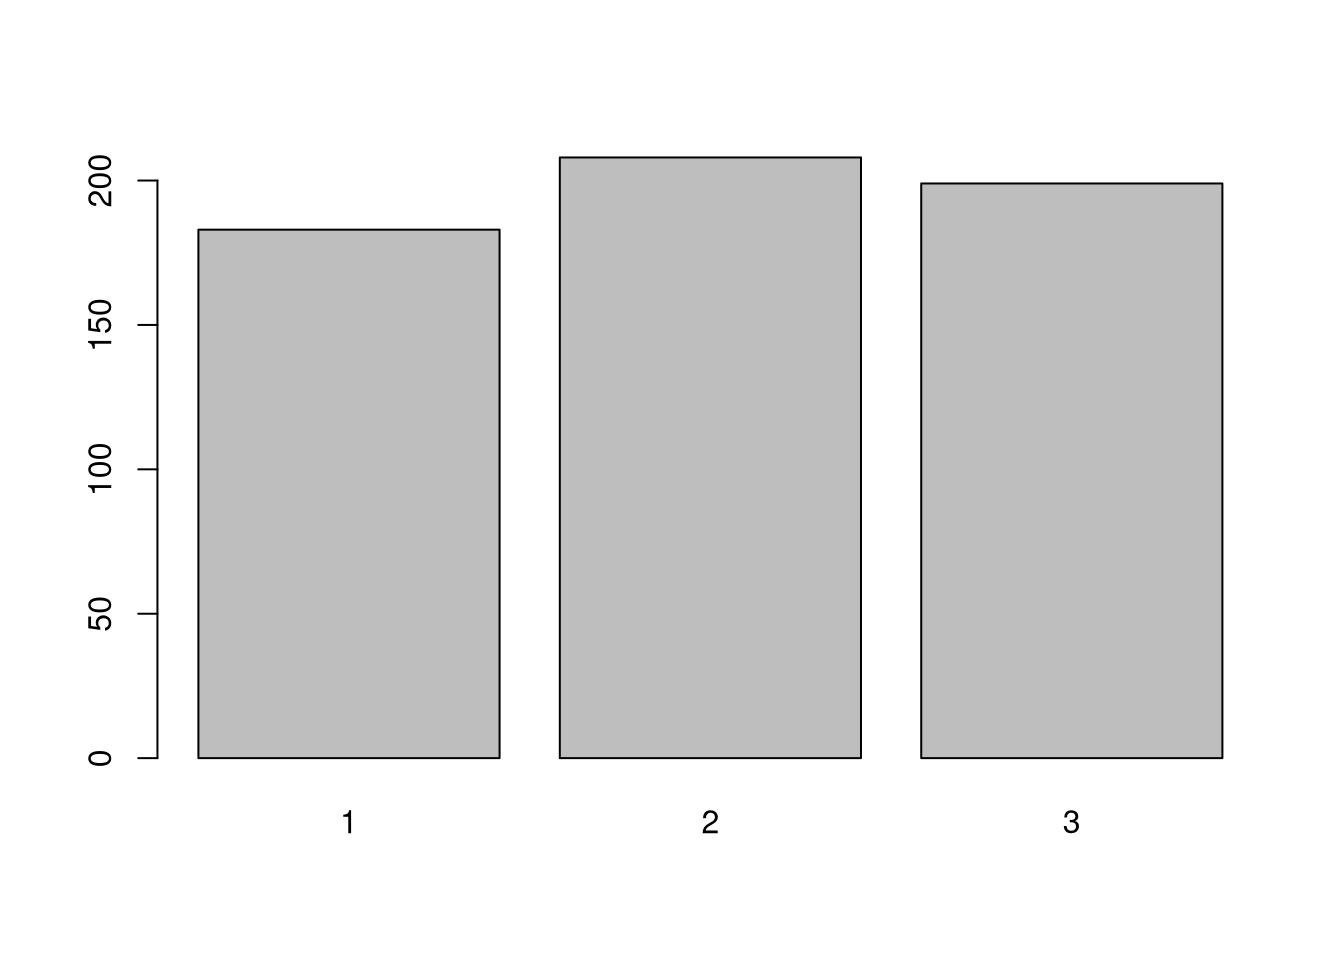
\includegraphics{Practica1_files/figure-latex/unnamed-chunk-2-1.pdf}
***** \#Ejericio 2:

\begin{itemize}
\tightlist
\item
  Estimar la probabilidad de ser mujer sabiendo que sobrevivió y
  comparar con la estimación de ser mujer a bordo del Titanic.
\end{itemize}

\begin{Shaded}
\begin{Highlighting}[]
\FunctionTok{setwd}\NormalTok{(}\StringTok{"\textasciitilde{}/Documents/FCEyN/Estadistica/Datos"}\NormalTok{)}
\NormalTok{titanic }\OtherTok{=} \FunctionTok{read.csv}\NormalTok{(}\StringTok{"datos\_titanic.csv"}\NormalTok{)}
\NormalTok{Psm }\OtherTok{=}\NormalTok{ titanic}\SpecialCharTok{$}\NormalTok{Sex[titanic}\SpecialCharTok{$}\NormalTok{Survived }\SpecialCharTok{==} \DecValTok{1}\NormalTok{]}

\FunctionTok{length}\NormalTok{(Psm[Psm }\SpecialCharTok{==} \StringTok{"female"}\NormalTok{]) }\SpecialCharTok{/} \FunctionTok{length}\NormalTok{(Psm) }
\end{Highlighting}
\end{Shaded}

\begin{verbatim}
## [1] 0.6812865
\end{verbatim}

\begin{itemize}
\tightlist
\item
  Hacer una tabla de contingencia entre las variables categóricas
  Survived y Pclass, luego hacer un grafico de barras.
\end{itemize}

\begin{Shaded}
\begin{Highlighting}[]
\NormalTok{t\_contringencia }\OtherTok{=} \FunctionTok{table}\NormalTok{(titanic}\SpecialCharTok{$}\NormalTok{Survived, titanic}\SpecialCharTok{$}\NormalTok{Pclass)}

\FunctionTok{barplot}\NormalTok{(t\_contringencia, }\AttributeTok{main=}\StringTok{"Survived vs Pclass"}\NormalTok{,}\AttributeTok{legend =} \FunctionTok{c}\NormalTok{(}\StringTok{"no survived"}\NormalTok{,}\StringTok{"survived"}\NormalTok{))}
\end{Highlighting}
\end{Shaded}

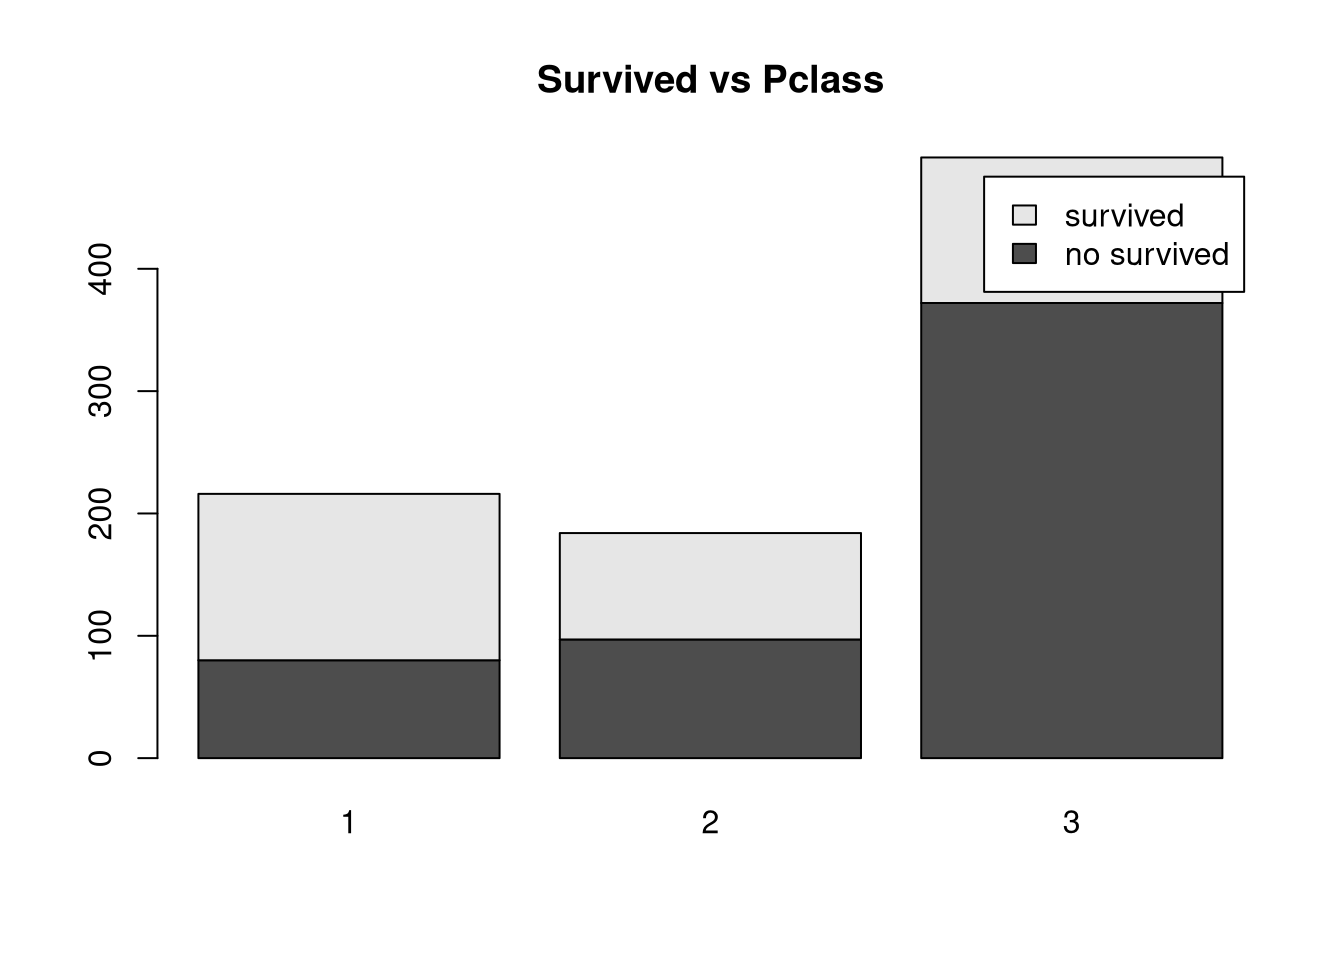
\includegraphics{Practica1_files/figure-latex/unnamed-chunk-4-1.pdf}
***** Ejercicio 3:

\begin{itemize}
\tightlist
\item
  Comparar los dos conjuntos de datos mediante histogramas y boxplots,
  graficando los boxplots en paralelo
\end{itemize}

\begin{Shaded}
\begin{Highlighting}[]
\FunctionTok{setwd}\NormalTok{(}\StringTok{"\textasciitilde{}/Documents/FCEyN/Estadistica/Datos"}\NormalTok{)}
\FunctionTok{library}\NormalTok{(}\StringTok{"ggplot2"}\NormalTok{)}
\NormalTok{iridio }\OtherTok{=} \FunctionTok{read.table}\NormalTok{(}\StringTok{"iridio.txt"}\NormalTok{,}\AttributeTok{header =} \ConstantTok{TRUE}\NormalTok{)}
\NormalTok{rodio }\OtherTok{=} \FunctionTok{read.table}\NormalTok{(}\StringTok{"rodio.txt"}\NormalTok{, }\AttributeTok{header =} \ConstantTok{TRUE}\NormalTok{)}
\NormalTok{iridio }\OtherTok{=}\NormalTok{ iridio}\SpecialCharTok{$}\NormalTok{iridio}
\NormalTok{rodio }\OtherTok{=}\NormalTok{ rodio}\SpecialCharTok{$}\NormalTok{rodio}

\FunctionTok{hist}\NormalTok{(iridio, }\AttributeTok{main =} \StringTok{"Histogram of Iridio"}\NormalTok{, }\AttributeTok{freq =} \ConstantTok{FALSE}\NormalTok{, }\AttributeTok{xlab =} \StringTok{"Iridio"}\NormalTok{)}
\end{Highlighting}
\end{Shaded}

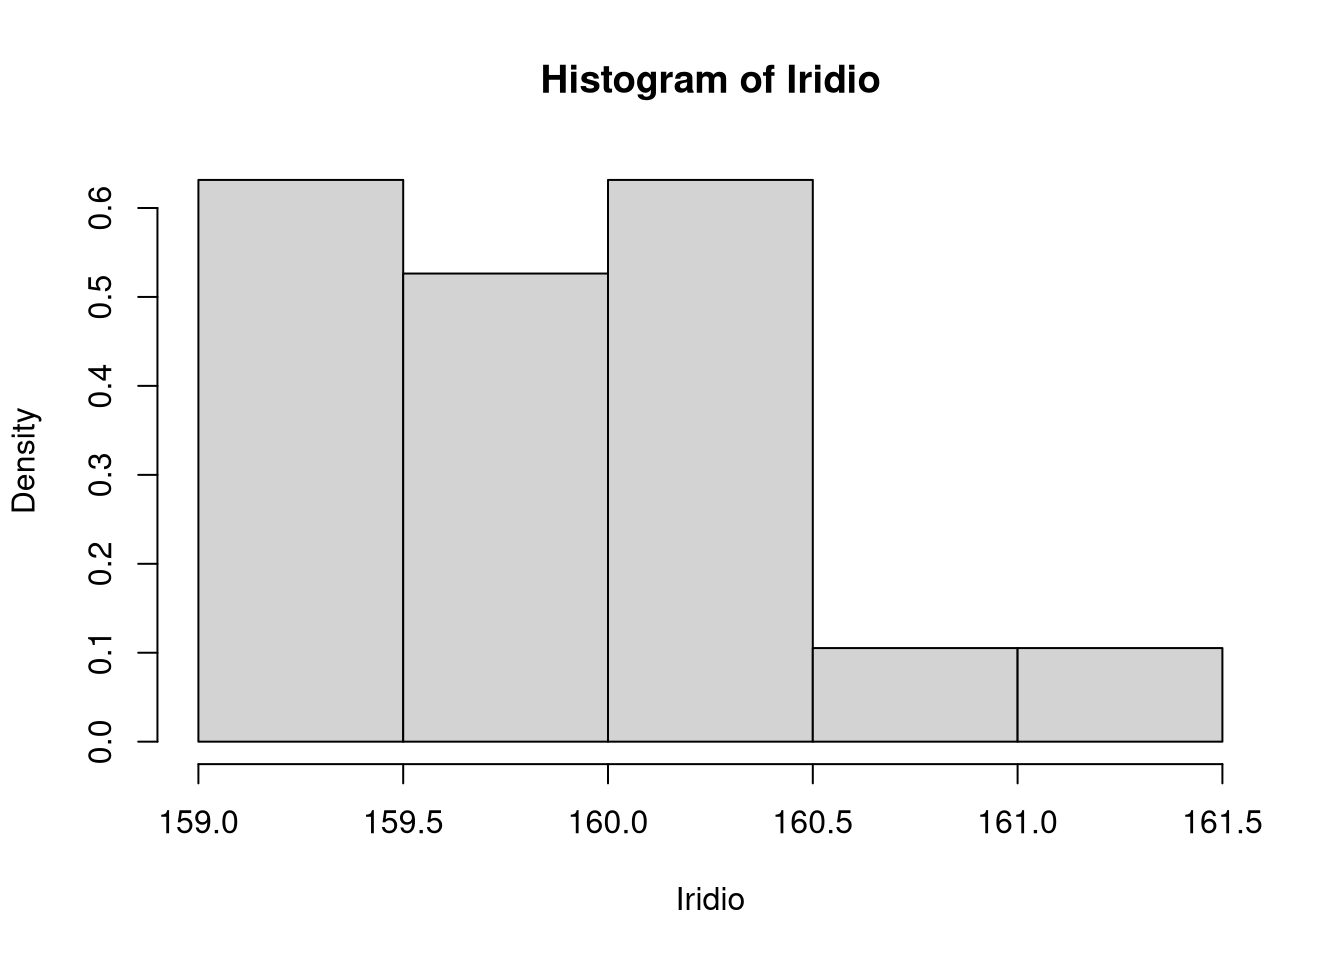
\includegraphics{Practica1_files/figure-latex/unnamed-chunk-5-1.pdf}

\begin{Shaded}
\begin{Highlighting}[]
\FunctionTok{hist}\NormalTok{(rodio, }\AttributeTok{main =} \StringTok{"Histogram of Rodio"}\NormalTok{, }\AttributeTok{freq =} \ConstantTok{FALSE}\NormalTok{, }\AttributeTok{xlab =} \StringTok{"Rodio"}\NormalTok{)}
\end{Highlighting}
\end{Shaded}

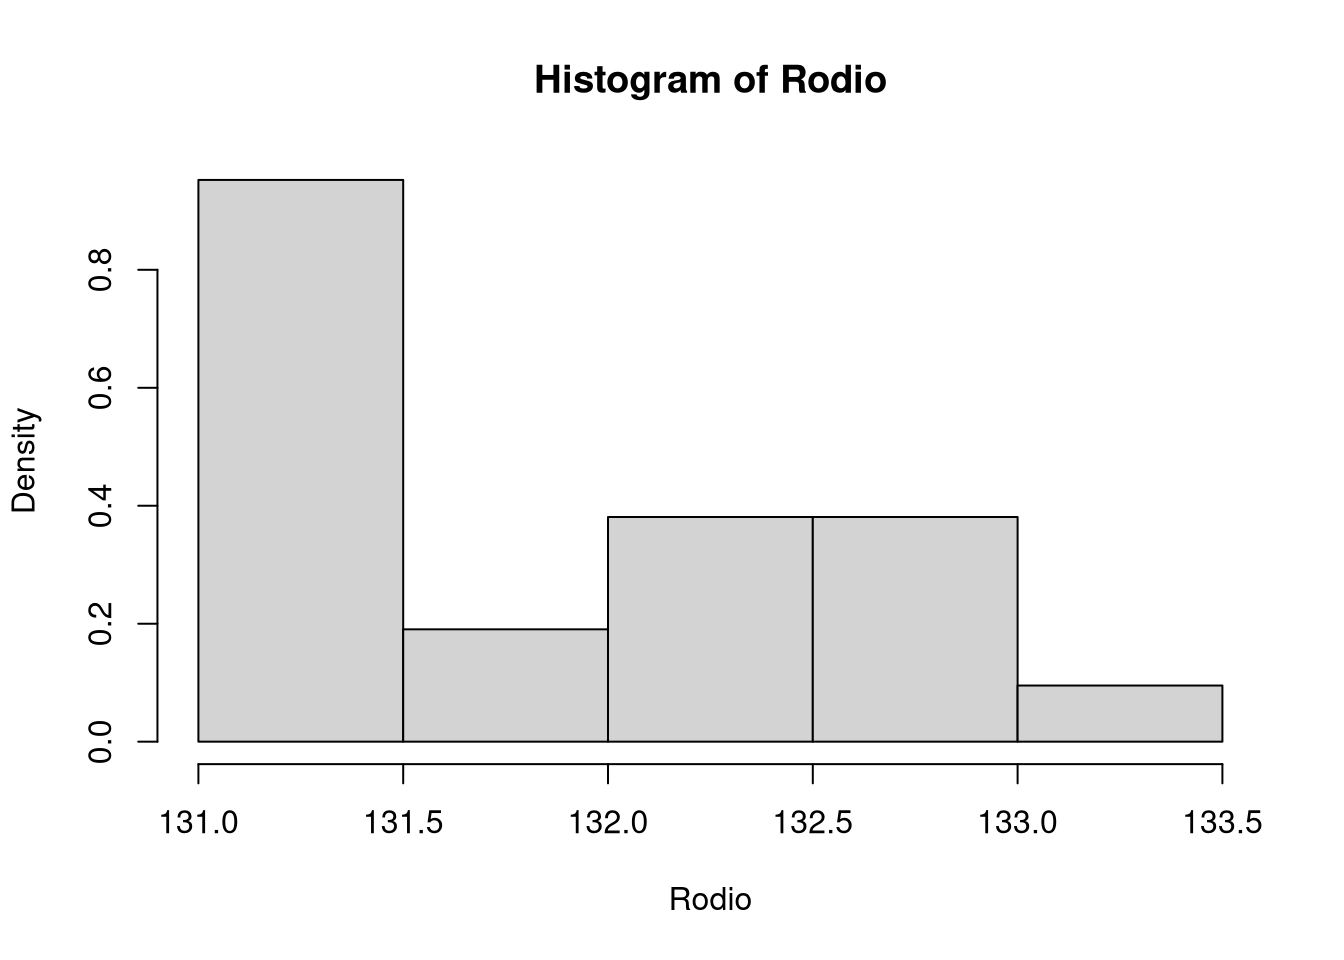
\includegraphics{Practica1_files/figure-latex/unnamed-chunk-5-2.pdf}

\begin{Shaded}
\begin{Highlighting}[]
\FunctionTok{boxplot}\NormalTok{(iridio, rodio, }\AttributeTok{main=} \StringTok{"Iridio y Rodio"}\NormalTok{)}
\end{Highlighting}
\end{Shaded}

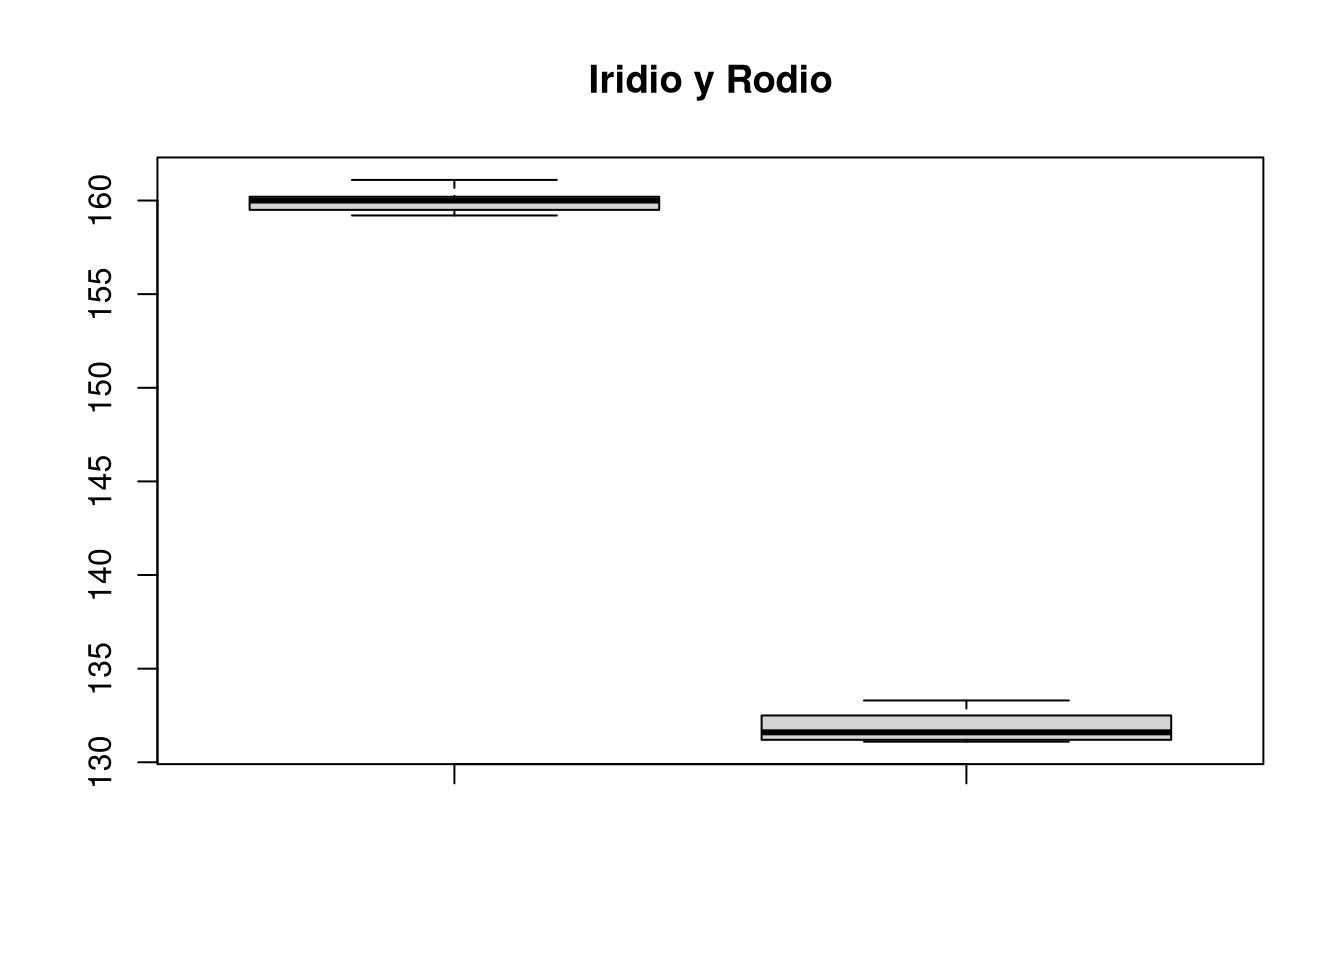
\includegraphics{Practica1_files/figure-latex/unnamed-chunk-5-3.pdf}

\begin{itemize}
\tightlist
\item
  Hallar las medias, las medianas y las medias podadas al 10 \% y 20 \%
  muestrales. Comparar.
\end{itemize}

\begin{Shaded}
\begin{Highlighting}[]
\NormalTok{t }\OtherTok{=} \FunctionTok{matrix}\NormalTok{(}\AttributeTok{nrow =} \DecValTok{2}\NormalTok{,}\AttributeTok{ncol =} \DecValTok{4}\NormalTok{, }\AttributeTok{byrow =} \ConstantTok{TRUE}\NormalTok{)}

\NormalTok{t[}\DecValTok{1}\NormalTok{,}\DecValTok{1}\NormalTok{] }\OtherTok{=} \FunctionTok{mean}\NormalTok{(iridio)}
\NormalTok{t[}\DecValTok{2}\NormalTok{,}\DecValTok{1}\NormalTok{] }\OtherTok{=} \FunctionTok{mean}\NormalTok{(rodio)}
\NormalTok{t[}\DecValTok{1}\NormalTok{,}\DecValTok{2}\NormalTok{] }\OtherTok{=} \FunctionTok{median}\NormalTok{(iridio)}
\NormalTok{t[}\DecValTok{2}\NormalTok{,}\DecValTok{2}\NormalTok{] }\OtherTok{=} \FunctionTok{median}\NormalTok{(rodio)}
\NormalTok{t[}\DecValTok{1}\NormalTok{,}\DecValTok{3}\NormalTok{] }\OtherTok{=} \FunctionTok{mean}\NormalTok{(iridio, }\AttributeTok{trim =} \FloatTok{0.1}\NormalTok{)}
\NormalTok{t[}\DecValTok{2}\NormalTok{,}\DecValTok{3}\NormalTok{] }\OtherTok{=} \FunctionTok{mean}\NormalTok{(rodio, }\AttributeTok{trim =} \FloatTok{0.1}\NormalTok{)}
\NormalTok{t[}\DecValTok{1}\NormalTok{,}\DecValTok{4}\NormalTok{] }\OtherTok{=} \FunctionTok{mean}\NormalTok{(iridio, }\AttributeTok{trim =} \FloatTok{0.2}\NormalTok{)}
\NormalTok{t[}\DecValTok{2}\NormalTok{,}\DecValTok{4}\NormalTok{] }\OtherTok{=} \FunctionTok{mean}\NormalTok{(rodio, }\AttributeTok{trim =} \FloatTok{0.2}\NormalTok{)}

\NormalTok{t }\OtherTok{=} \FunctionTok{as.table}\NormalTok{(t)}
\FunctionTok{rownames}\NormalTok{(t) }\OtherTok{=} \FunctionTok{c}\NormalTok{(}\StringTok{"Iridio"}\NormalTok{,}\StringTok{"Rodio"}\NormalTok{)}
\FunctionTok{colnames}\NormalTok{(t) }\OtherTok{=} \FunctionTok{c}\NormalTok{(}\StringTok{"Media"}\NormalTok{,}\StringTok{"Mediana"}\NormalTok{,}\StringTok{"Media01Podada"}\NormalTok{,}\StringTok{"Media02Podada"}\NormalTok{)}
\NormalTok{t}
\end{Highlighting}
\end{Shaded}

\begin{verbatim}
##           Media  Mediana Media01Podada Media02Podada
## Iridio 159.9158 160.0000      159.8882      159.8692
## Rodio  131.8762 131.6000      131.8176      131.7692
\end{verbatim}

\begin{itemize}
\tightlist
\item
  Hallar los desvı́os estándares, las distancias intercuartiles y las MAD
  muestrales como medidas de dispersión
\end{itemize}

\begin{Shaded}
\begin{Highlighting}[]
\NormalTok{m }\OtherTok{=} \FunctionTok{matrix}\NormalTok{(}\AttributeTok{nrow =} \DecValTok{2}\NormalTok{,}\AttributeTok{ncol=}\DecValTok{3}\NormalTok{)}

\NormalTok{m[}\DecValTok{1}\NormalTok{,}\DecValTok{1}\NormalTok{] }\OtherTok{=} \FunctionTok{sd}\NormalTok{(iridio)}
\NormalTok{m[}\DecValTok{2}\NormalTok{,}\DecValTok{1}\NormalTok{] }\OtherTok{=} \FunctionTok{sd}\NormalTok{(rodio)}
\NormalTok{m[}\DecValTok{1}\NormalTok{,}\DecValTok{2}\NormalTok{] }\OtherTok{=} \FunctionTok{IQR}\NormalTok{(iridio)}
\NormalTok{m[}\DecValTok{2}\NormalTok{,}\DecValTok{2}\NormalTok{] }\OtherTok{=} \FunctionTok{IQR}\NormalTok{(rodio)}
\NormalTok{m[}\DecValTok{1}\NormalTok{,}\DecValTok{3}\NormalTok{] }\OtherTok{=} \FunctionTok{mad}\NormalTok{(iridio)}
\NormalTok{m[}\DecValTok{2}\NormalTok{,}\DecValTok{3}\NormalTok{] }\OtherTok{=} \FunctionTok{mad}\NormalTok{(rodio)}

\NormalTok{m }\OtherTok{=} \FunctionTok{as.table}\NormalTok{(m)}
\FunctionTok{rownames}\NormalTok{(m) }\OtherTok{=} \FunctionTok{c}\NormalTok{(}\StringTok{"Iridio"}\NormalTok{,}\StringTok{"Rodio"}\NormalTok{)}
\FunctionTok{colnames}\NormalTok{(m) }\OtherTok{=} \FunctionTok{c}\NormalTok{(}\StringTok{"desviación estándar"}\NormalTok{,}\StringTok{"Distancia IQ"}\NormalTok{,}\StringTok{"MAD"}\NormalTok{)}
\NormalTok{m}
\end{Highlighting}
\end{Shaded}

\begin{verbatim}
##        desviación estándar Distancia IQ       MAD
## Iridio           0.4901963    0.7000000 0.5930400
## Rodio            0.7509359    1.3000000 0.7413000
\end{verbatim}

\begin{itemize}
\tightlist
\item
  Hallar los cuantiles 0,90, 0,75, 0,50, 0,25 y 0,10
\end{itemize}

\begin{Shaded}
\begin{Highlighting}[]
\NormalTok{u }\OtherTok{=} \FunctionTok{matrix}\NormalTok{(}\AttributeTok{nrow =} \DecValTok{2}\NormalTok{,}\AttributeTok{ncol =} \DecValTok{5}\NormalTok{)}
\NormalTok{u[}\DecValTok{1}\NormalTok{,}\DecValTok{1}\NormalTok{] }\OtherTok{=} \FunctionTok{quantile}\NormalTok{(iridio,}\FloatTok{0.9}\NormalTok{)}
\NormalTok{u[}\DecValTok{2}\NormalTok{,}\DecValTok{1}\NormalTok{] }\OtherTok{=} \FunctionTok{quantile}\NormalTok{(rodio,}\FloatTok{0.9}\NormalTok{)}
\NormalTok{u[}\DecValTok{1}\NormalTok{,}\DecValTok{2}\NormalTok{] }\OtherTok{=} \FunctionTok{quantile}\NormalTok{(iridio,}\FloatTok{0.75}\NormalTok{)}
\NormalTok{u[}\DecValTok{2}\NormalTok{,}\DecValTok{2}\NormalTok{] }\OtherTok{=} \FunctionTok{quantile}\NormalTok{(rodio,}\FloatTok{0.75}\NormalTok{)}
\NormalTok{u[}\DecValTok{1}\NormalTok{,}\DecValTok{3}\NormalTok{] }\OtherTok{=} \FunctionTok{quantile}\NormalTok{(iridio,}\FloatTok{0.5}\NormalTok{)}
\NormalTok{u[}\DecValTok{2}\NormalTok{,}\DecValTok{3}\NormalTok{] }\OtherTok{=} \FunctionTok{quantile}\NormalTok{(rodio,}\FloatTok{0.5}\NormalTok{)}
\NormalTok{u[}\DecValTok{1}\NormalTok{,}\DecValTok{4}\NormalTok{] }\OtherTok{=} \FunctionTok{quantile}\NormalTok{(iridio,}\FloatTok{0.25}\NormalTok{)}
\NormalTok{u[}\DecValTok{2}\NormalTok{,}\DecValTok{4}\NormalTok{] }\OtherTok{=} \FunctionTok{quantile}\NormalTok{(rodio,}\FloatTok{0.25}\NormalTok{)}
\NormalTok{u[}\DecValTok{1}\NormalTok{,}\DecValTok{5}\NormalTok{] }\OtherTok{=} \FunctionTok{quantile}\NormalTok{(iridio,}\FloatTok{0.1}\NormalTok{)}
\NormalTok{u[}\DecValTok{2}\NormalTok{,}\DecValTok{5}\NormalTok{] }\OtherTok{=} \FunctionTok{quantile}\NormalTok{(rodio,}\FloatTok{0.1}\NormalTok{)}

\NormalTok{u }\OtherTok{=} \FunctionTok{as.table}\NormalTok{(u)}
\FunctionTok{rownames}\NormalTok{(u) }\OtherTok{=} \FunctionTok{c}\NormalTok{(}\StringTok{"Iridio"}\NormalTok{,}\StringTok{"Rodio"}\NormalTok{)}
\FunctionTok{colnames}\NormalTok{(u) }\OtherTok{=} \FunctionTok{c}\NormalTok{(}\StringTok{"0.9"}\NormalTok{,}\StringTok{"0.75"}\NormalTok{,}\StringTok{"0.50"}\NormalTok{,}\StringTok{"0.25"}\NormalTok{,}\StringTok{"0.1"}\NormalTok{)}
\NormalTok{u}
\end{Highlighting}
\end{Shaded}

\begin{verbatim}
##           0.9   0.75   0.50   0.25    0.1
## Iridio 160.44 160.20 160.00 159.50 159.46
## Rodio  133.00 132.50 131.60 131.20 131.10
\end{verbatim}

\begin{verbatim}
                                                    *****
\end{verbatim}

\hypertarget{ejericio-4}{%
\section{Ejericio 4:}\label{ejericio-4}}

\begin{itemize}
\tightlist
\item
  Realizar un histograma para las calorı́as de cada tipo de salchichas.
  ¿Observa grupos en algún gráfico? ¿Cuántos grupos observa? ¿Observa
  algún candidato a dato atı́pico? ¿Alguno de los histogramas tiene una
  caracterı́stica particular? .
\end{itemize}

\begin{Shaded}
\begin{Highlighting}[]
\CommentTok{\#Cargamos los datos}
\FunctionTok{setwd}\NormalTok{(}\StringTok{"\textasciitilde{}/Documents/FCEyN/Estadistica/Datos"}\NormalTok{)}
\NormalTok{salA }\OtherTok{=} \FunctionTok{read.table}\NormalTok{(}\StringTok{"salchichas\_A.txt"}\NormalTok{,}\AttributeTok{header =} \ConstantTok{TRUE}\NormalTok{)}
\NormalTok{salB }\OtherTok{=} \FunctionTok{read.table}\NormalTok{(}\StringTok{"salchichas\_B.txt"}\NormalTok{,}\AttributeTok{header =} \ConstantTok{TRUE}\NormalTok{)}
\NormalTok{salC }\OtherTok{=} \FunctionTok{read.table}\NormalTok{(}\StringTok{"salchichas\_C.txt"}\NormalTok{,}\AttributeTok{header =} \ConstantTok{TRUE}\NormalTok{)}
\end{Highlighting}
\end{Shaded}

\begin{Shaded}
\begin{Highlighting}[]
\FunctionTok{hist}\NormalTok{(salA}\SpecialCharTok{$}\NormalTok{CALORIAS.A,}\AttributeTok{main =} \StringTok{"Histograma de A"}\NormalTok{,}\AttributeTok{xlab =} \StringTok{"Calorias"}\NormalTok{)}
\end{Highlighting}
\end{Shaded}

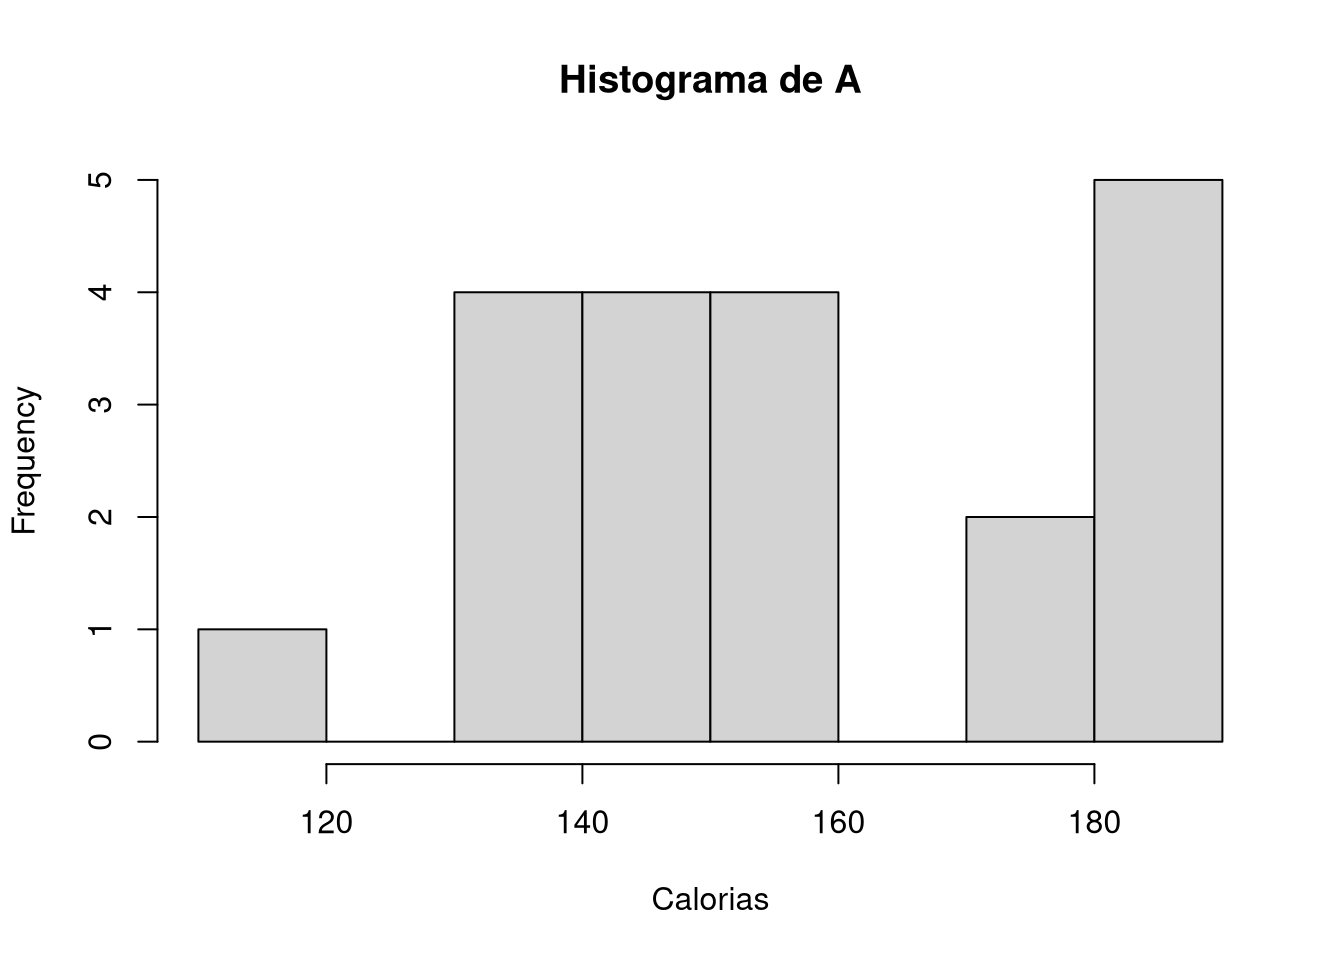
\includegraphics{Practica1_files/figure-latex/unnamed-chunk-10-1.pdf}

\begin{Shaded}
\begin{Highlighting}[]
\FunctionTok{hist}\NormalTok{(salB}\SpecialCharTok{$}\NormalTok{CALORIAS.B,}\AttributeTok{main =} \StringTok{"Histograma de B"}\NormalTok{,}\AttributeTok{xlab =} \StringTok{"Calorias"}\NormalTok{)}
\end{Highlighting}
\end{Shaded}

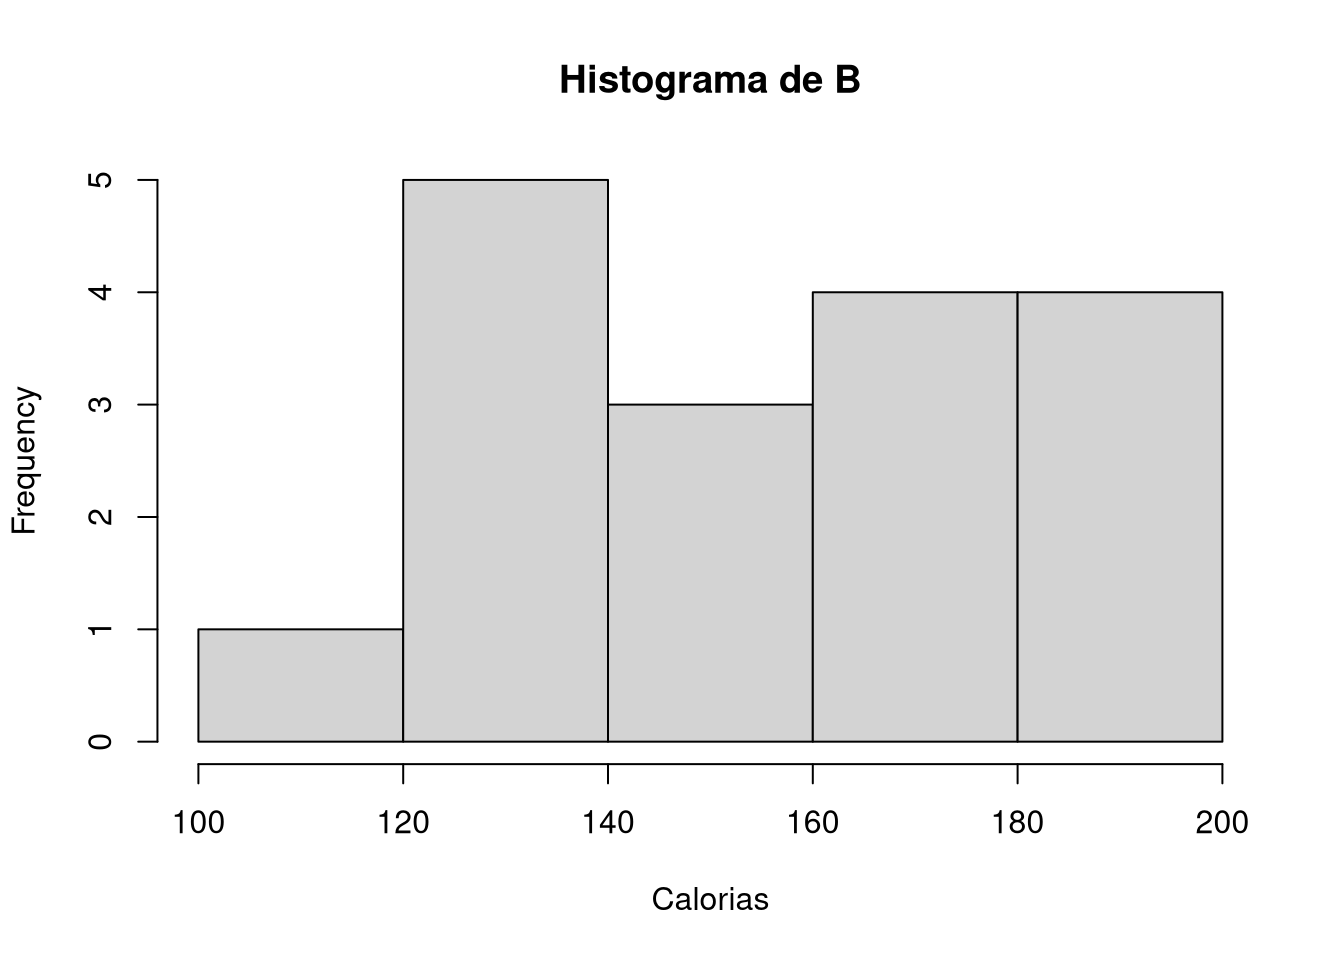
\includegraphics{Practica1_files/figure-latex/unnamed-chunk-10-2.pdf}

\begin{Shaded}
\begin{Highlighting}[]
\FunctionTok{hist}\NormalTok{(salC}\SpecialCharTok{$}\NormalTok{CALORIAS.C,}\AttributeTok{main =} \StringTok{"Histograma de C"}\NormalTok{,}\AttributeTok{xlab =} \StringTok{"Calorias"}\NormalTok{)}
\end{Highlighting}
\end{Shaded}

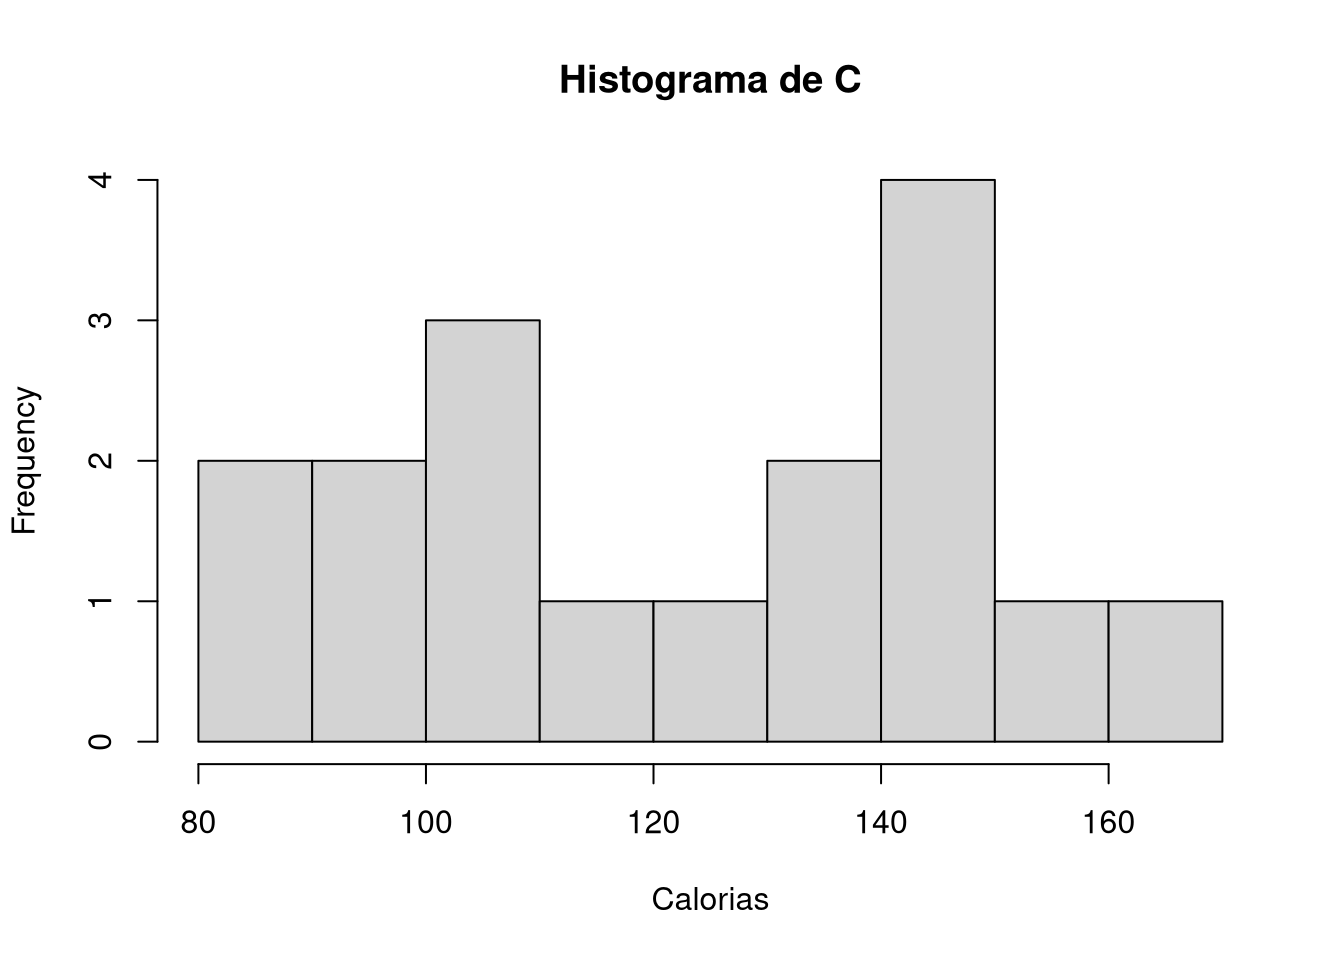
\includegraphics{Practica1_files/figure-latex/unnamed-chunk-10-3.pdf} *
Realizar los boxplots paralelos para las calorı́as.

\begin{Shaded}
\begin{Highlighting}[]
\FunctionTok{boxplot}\NormalTok{(salA}\SpecialCharTok{$}\NormalTok{CALORIAS.A,salB}\SpecialCharTok{$}\NormalTok{CALORIAS.B,salC}\SpecialCharTok{$}\NormalTok{CALORIAS.C)}
\end{Highlighting}
\end{Shaded}

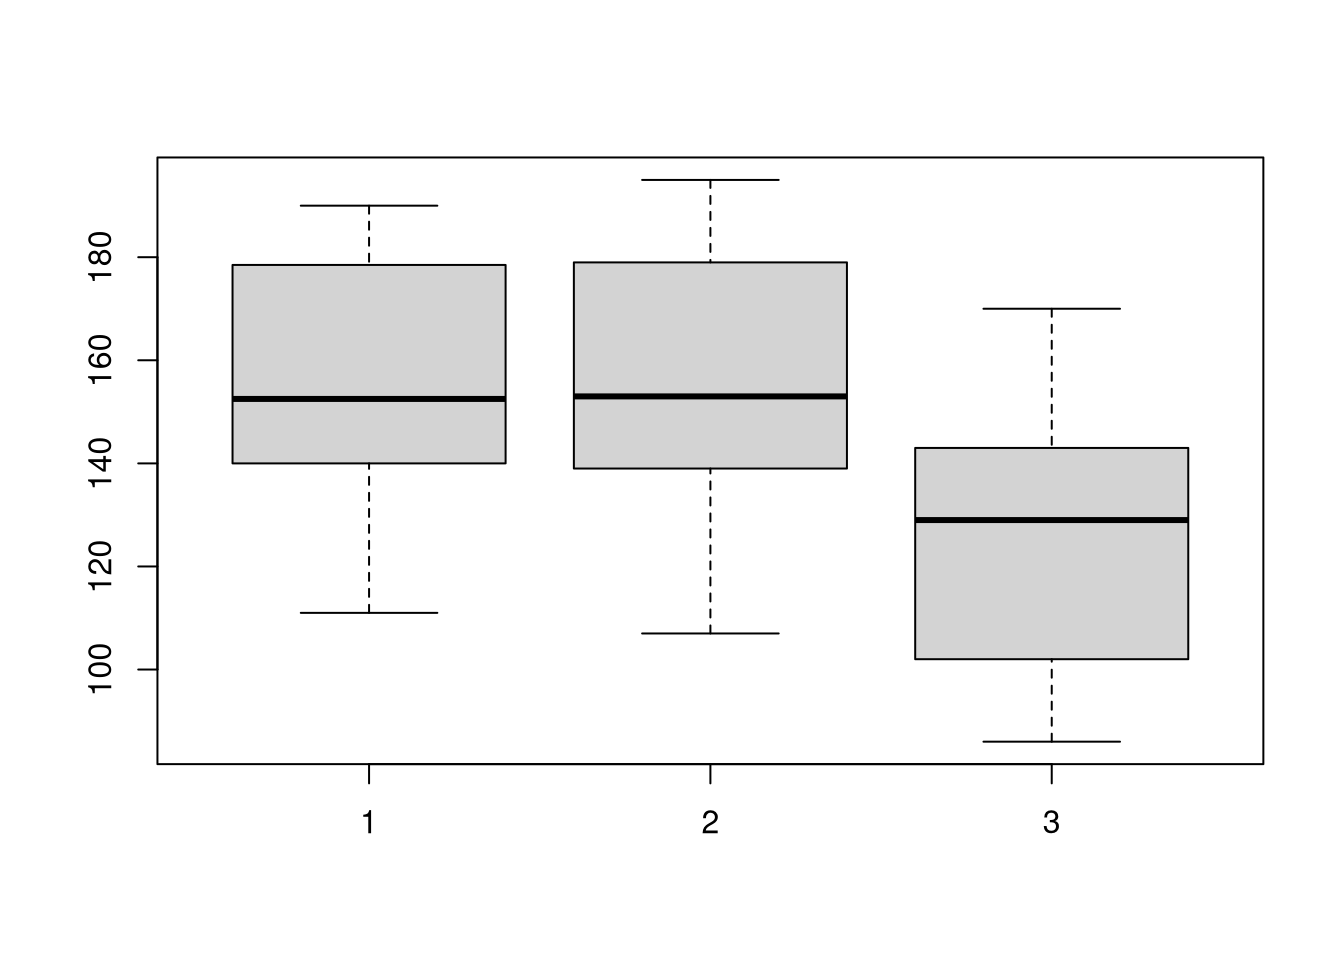
\includegraphics{Practica1_files/figure-latex/unnamed-chunk-11-1.pdf}

\begin{itemize}
\tightlist
\item
  Repetimos con la cantidad de sodio.
\end{itemize}

\begin{Shaded}
\begin{Highlighting}[]
\FunctionTok{hist}\NormalTok{(salA}\SpecialCharTok{$}\NormalTok{SODIO.A,}\AttributeTok{main =} \StringTok{"Histograma de A"}\NormalTok{,}\AttributeTok{xlab =} \StringTok{"Sodio"}\NormalTok{)}
\end{Highlighting}
\end{Shaded}

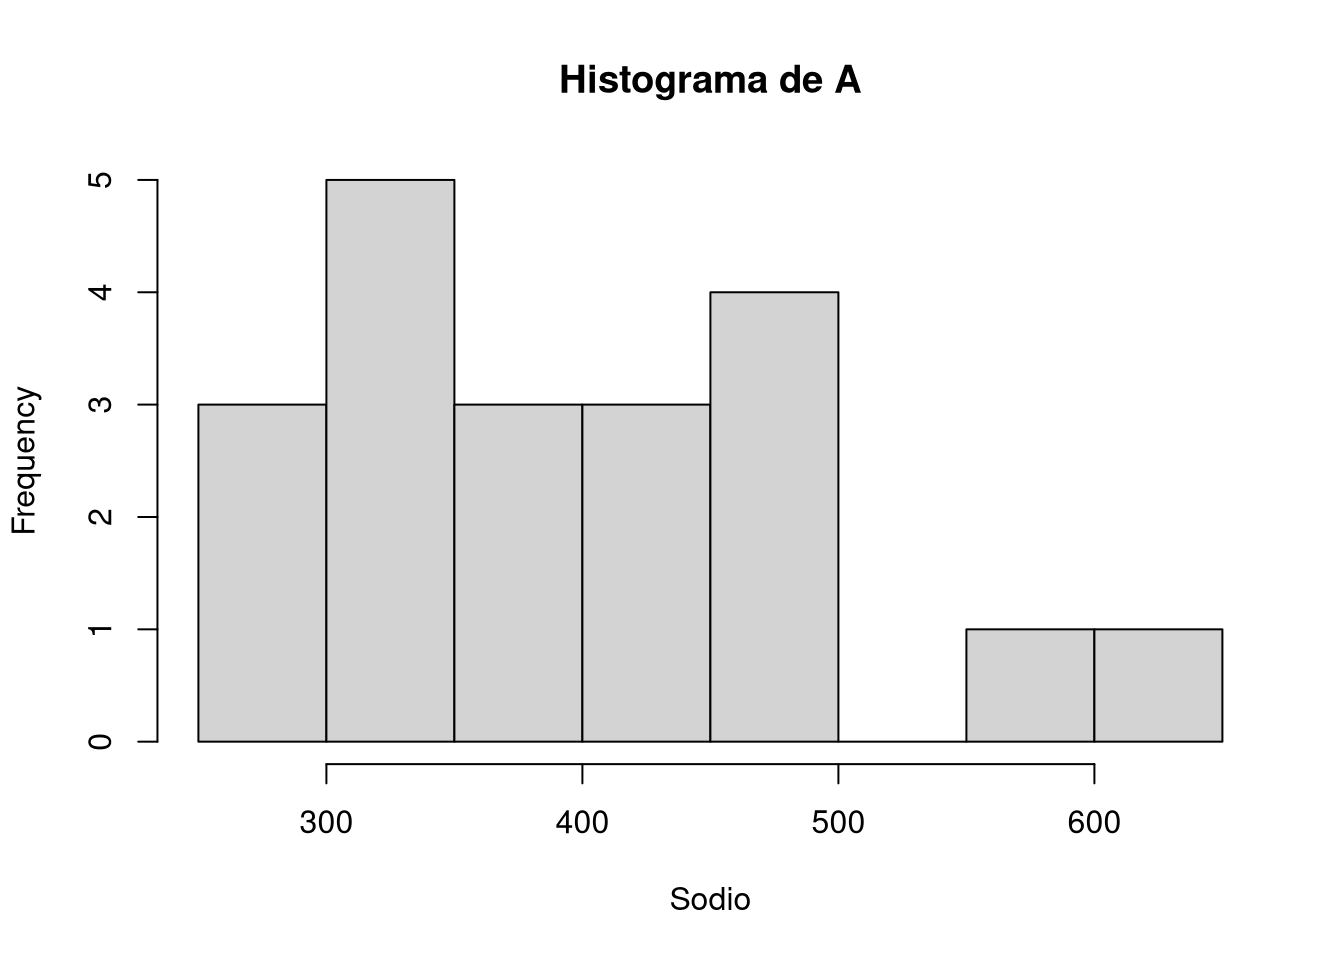
\includegraphics{Practica1_files/figure-latex/unnamed-chunk-12-1.pdf}

\begin{Shaded}
\begin{Highlighting}[]
\FunctionTok{hist}\NormalTok{(salB}\SpecialCharTok{$}\NormalTok{SODIO.B,}\AttributeTok{main =} \StringTok{"Histograma de B"}\NormalTok{,}\AttributeTok{xlab =} \StringTok{"Sodio"}\NormalTok{)}
\end{Highlighting}
\end{Shaded}

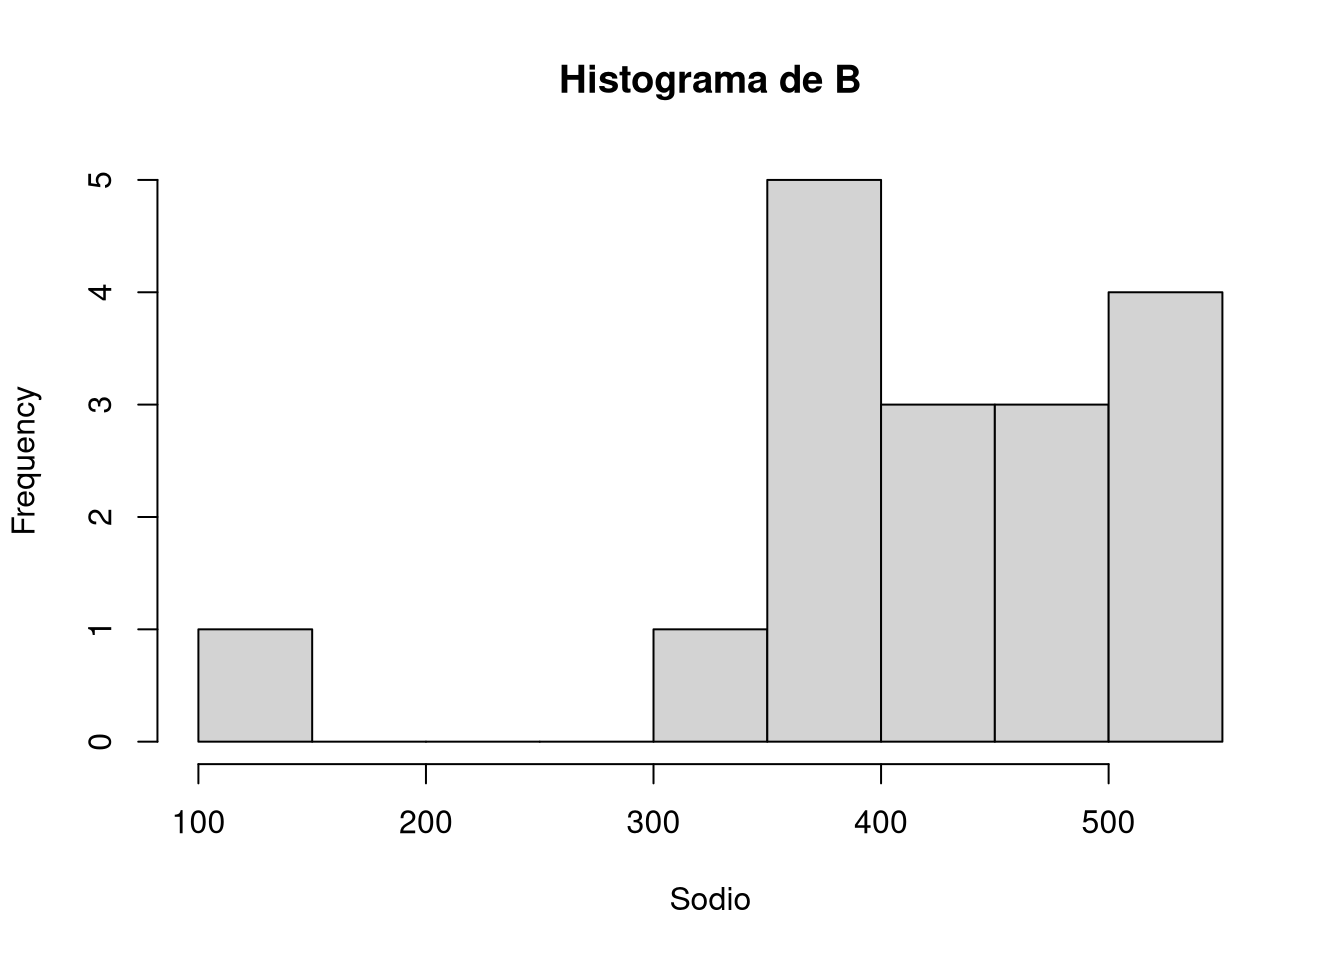
\includegraphics{Practica1_files/figure-latex/unnamed-chunk-12-2.pdf}

\begin{Shaded}
\begin{Highlighting}[]
\FunctionTok{hist}\NormalTok{(salC}\SpecialCharTok{$}\NormalTok{SODIO.C,}\AttributeTok{main =} \StringTok{"Histograma de C"}\NormalTok{,}\AttributeTok{xlab =} \StringTok{"Sodio"}\NormalTok{)}
\end{Highlighting}
\end{Shaded}

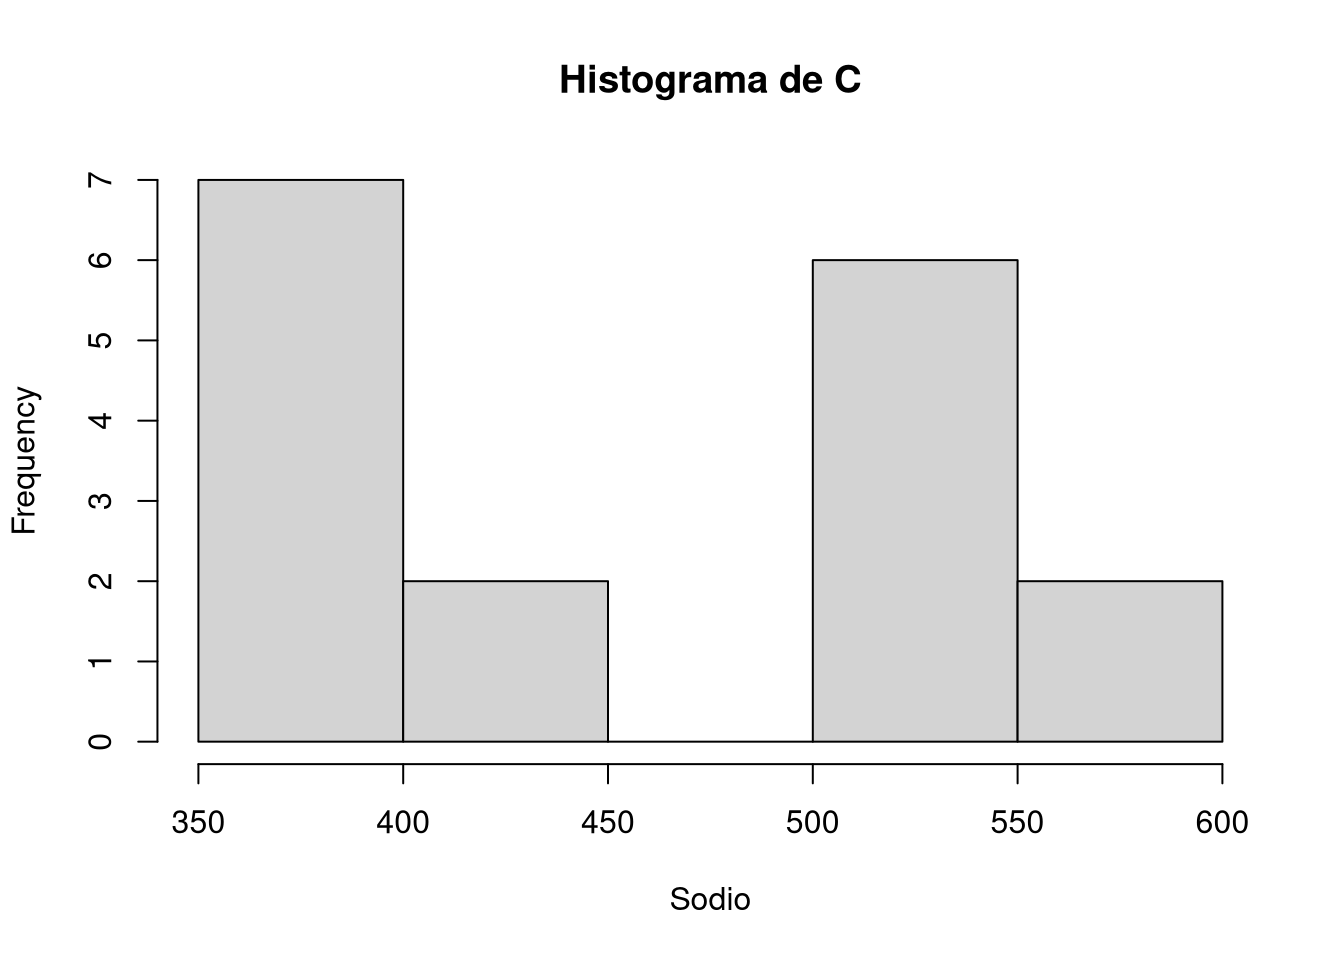
\includegraphics{Practica1_files/figure-latex/unnamed-chunk-12-3.pdf}

\begin{Shaded}
\begin{Highlighting}[]
\FunctionTok{boxplot}\NormalTok{(salA}\SpecialCharTok{$}\NormalTok{SODIO.A,salB}\SpecialCharTok{$}\NormalTok{SODIO.B,salC}\SpecialCharTok{$}\NormalTok{SODIO.C)}
\end{Highlighting}
\end{Shaded}

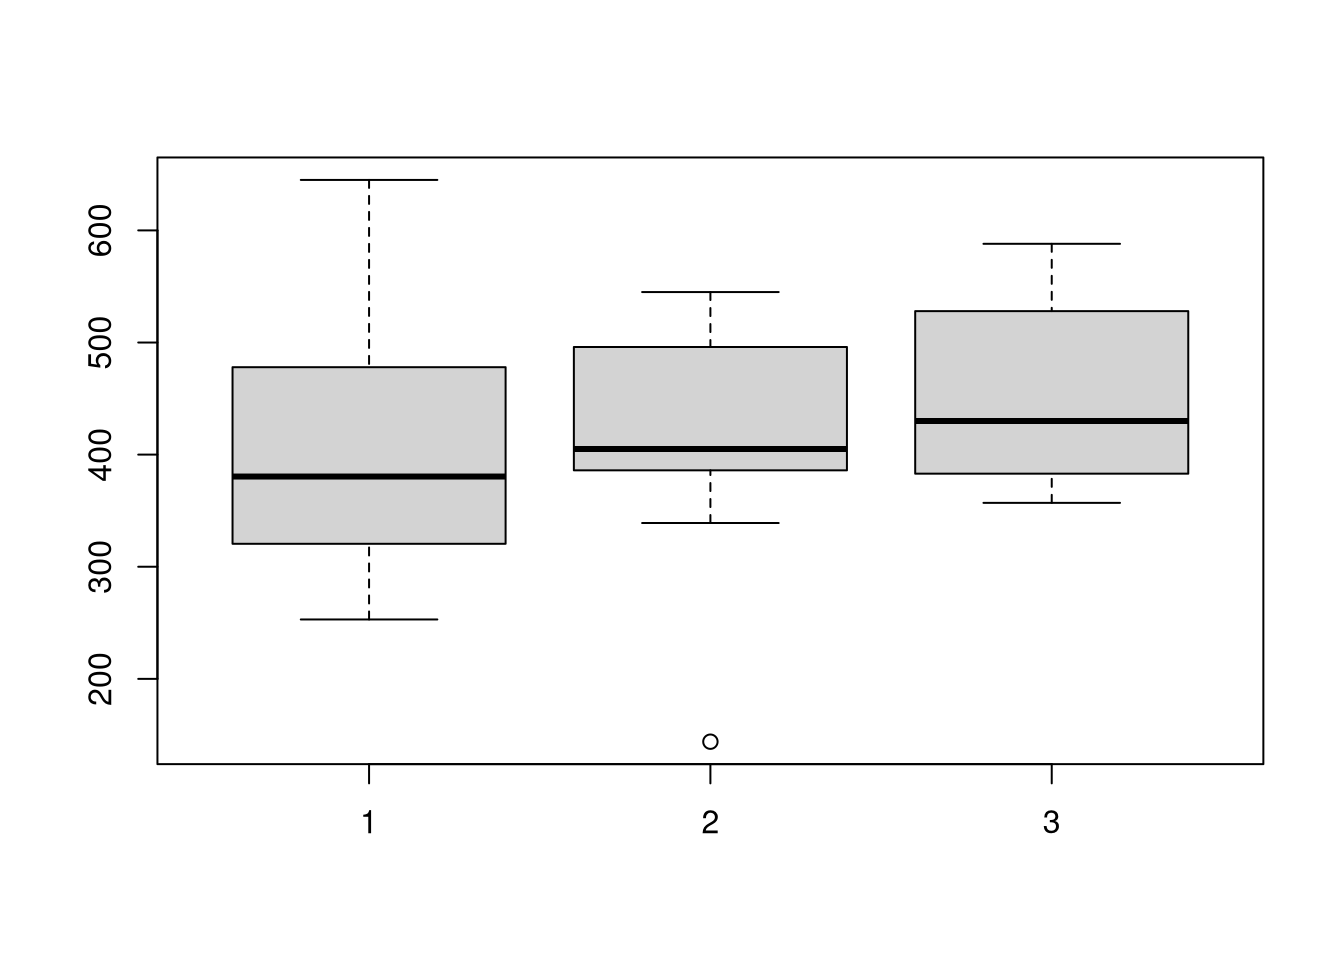
\includegraphics{Practica1_files/figure-latex/unnamed-chunk-13-1.pdf}
***** \# Ejericio 5:

\begin{itemize}
\tightlist
\item
  Cargamos los datos.
\end{itemize}

\begin{Shaded}
\begin{Highlighting}[]
\FunctionTok{setwd}\NormalTok{(}\StringTok{"\textasciitilde{}/Documents/FCEyN/Estadistica/Datos"}\NormalTok{)}
\NormalTok{est }\OtherTok{=} \FunctionTok{read.table}\NormalTok{(}\StringTok{"estudiantes.txt"}\NormalTok{, }\AttributeTok{header =} \ConstantTok{TRUE}\NormalTok{)}
\end{Highlighting}
\end{Shaded}

\begin{itemize}
\tightlist
\item
  Estudiar si la distribución de los conjuntos de datos para ambos
  grupos es normal.
\end{itemize}

\begin{Shaded}
\begin{Highlighting}[]
\FunctionTok{hist}\NormalTok{(est}\SpecialCharTok{$}\NormalTok{GRUPO1, }\AttributeTok{main =} \StringTok{"hist del grupo A"}\NormalTok{)}
\end{Highlighting}
\end{Shaded}

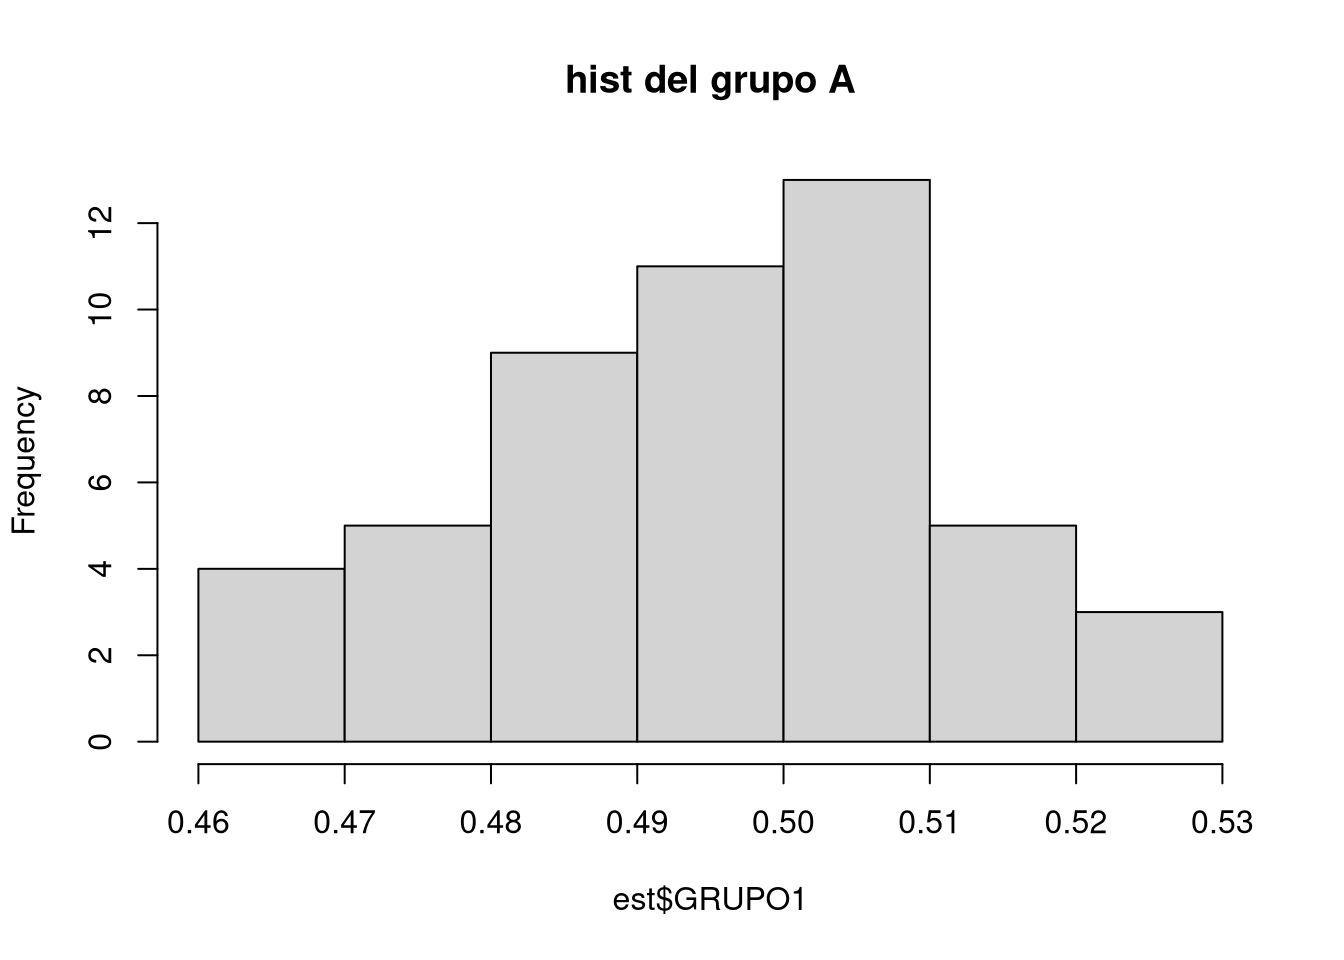
\includegraphics{Practica1_files/figure-latex/unnamed-chunk-15-1.pdf}

\begin{Shaded}
\begin{Highlighting}[]
\FunctionTok{hist}\NormalTok{(est}\SpecialCharTok{$}\NormalTok{GRUPO2, }\AttributeTok{main =} \StringTok{"hist del grupo B"}\NormalTok{)}
\end{Highlighting}
\end{Shaded}

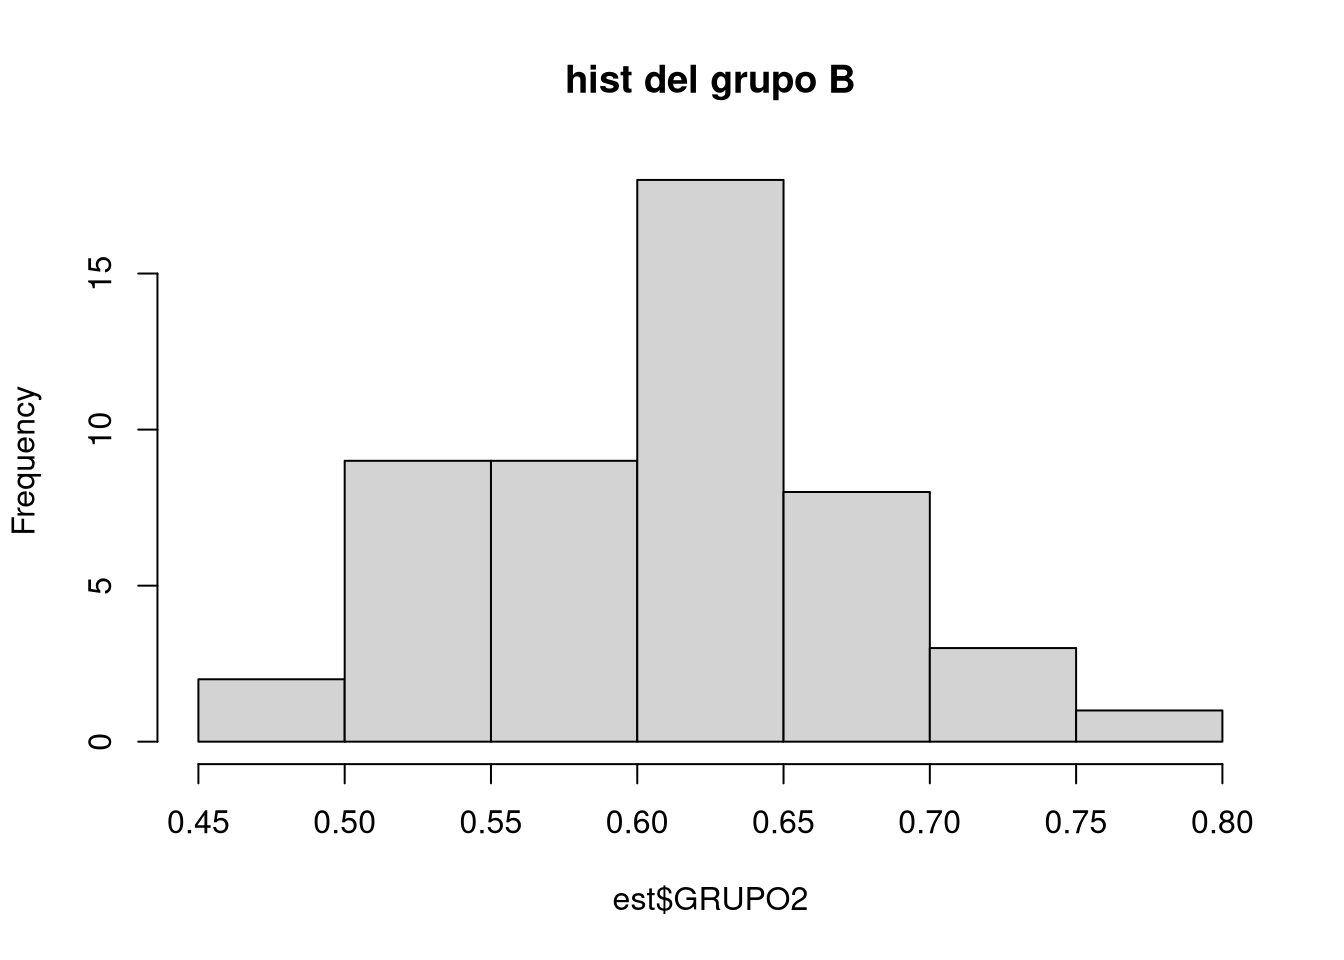
\includegraphics{Practica1_files/figure-latex/unnamed-chunk-15-2.pdf}

\begin{Shaded}
\begin{Highlighting}[]
\FunctionTok{qqnorm}\NormalTok{(est}\SpecialCharTok{$}\NormalTok{GRUPO1, }\AttributeTok{main =} \StringTok{"Normal qq grupo A"}\NormalTok{)}
\FunctionTok{qqline}\NormalTok{(est}\SpecialCharTok{$}\NormalTok{GRUPO1,}\AttributeTok{col=}\StringTok{"red"}\NormalTok{)}
\end{Highlighting}
\end{Shaded}

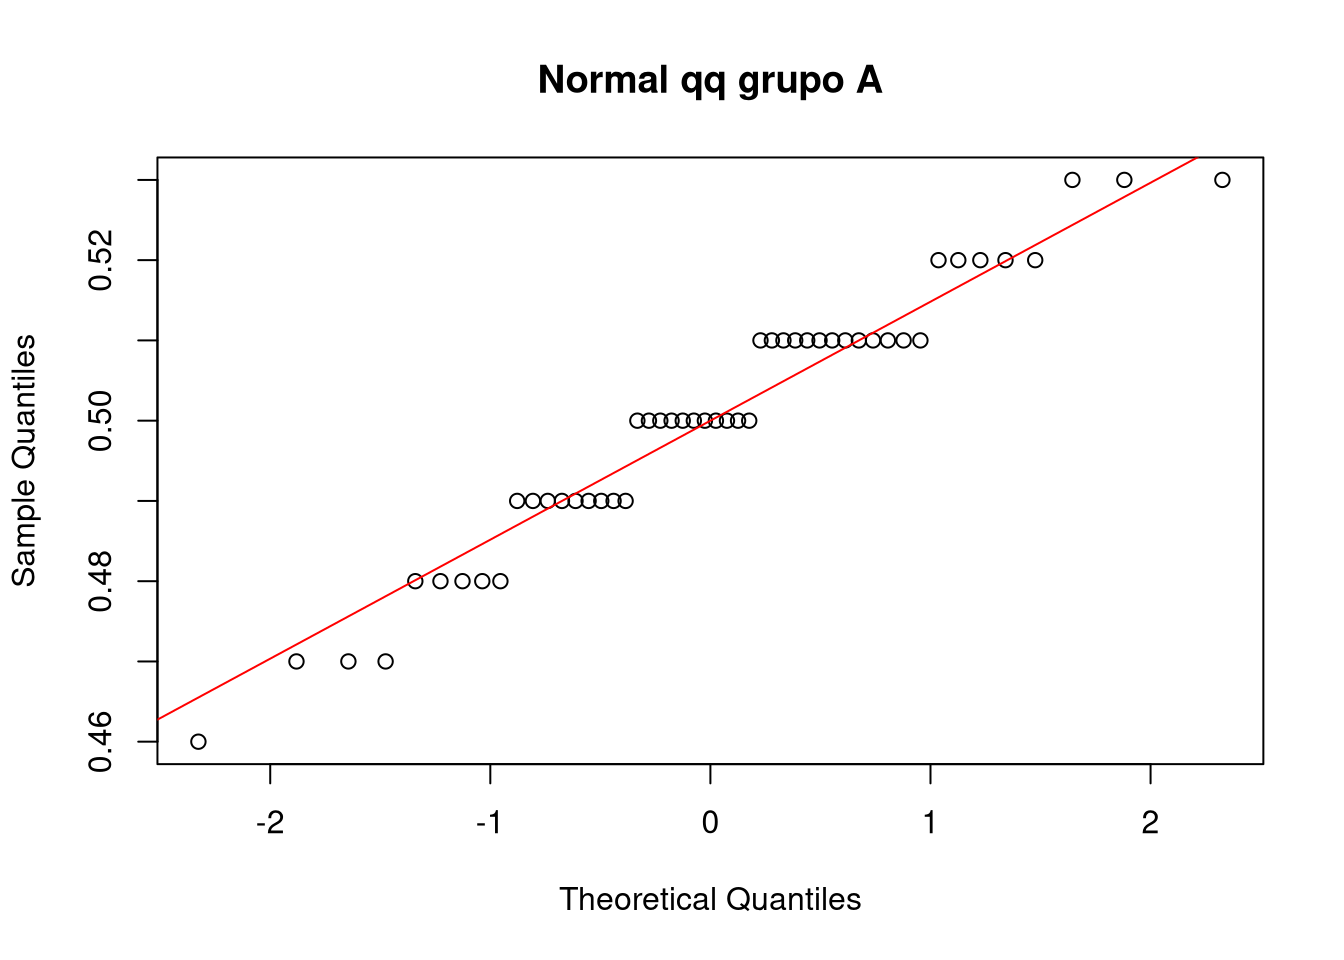
\includegraphics{Practica1_files/figure-latex/unnamed-chunk-15-3.pdf}

\begin{Shaded}
\begin{Highlighting}[]
\FunctionTok{qqnorm}\NormalTok{(est}\SpecialCharTok{$}\NormalTok{GRUPO2, }\AttributeTok{main =} \StringTok{"Normal qq grupo A"}\NormalTok{)}
\FunctionTok{qqline}\NormalTok{(est}\SpecialCharTok{$}\NormalTok{GRUPO2,}\AttributeTok{col=}\StringTok{"red"}\NormalTok{)}
\end{Highlighting}
\end{Shaded}

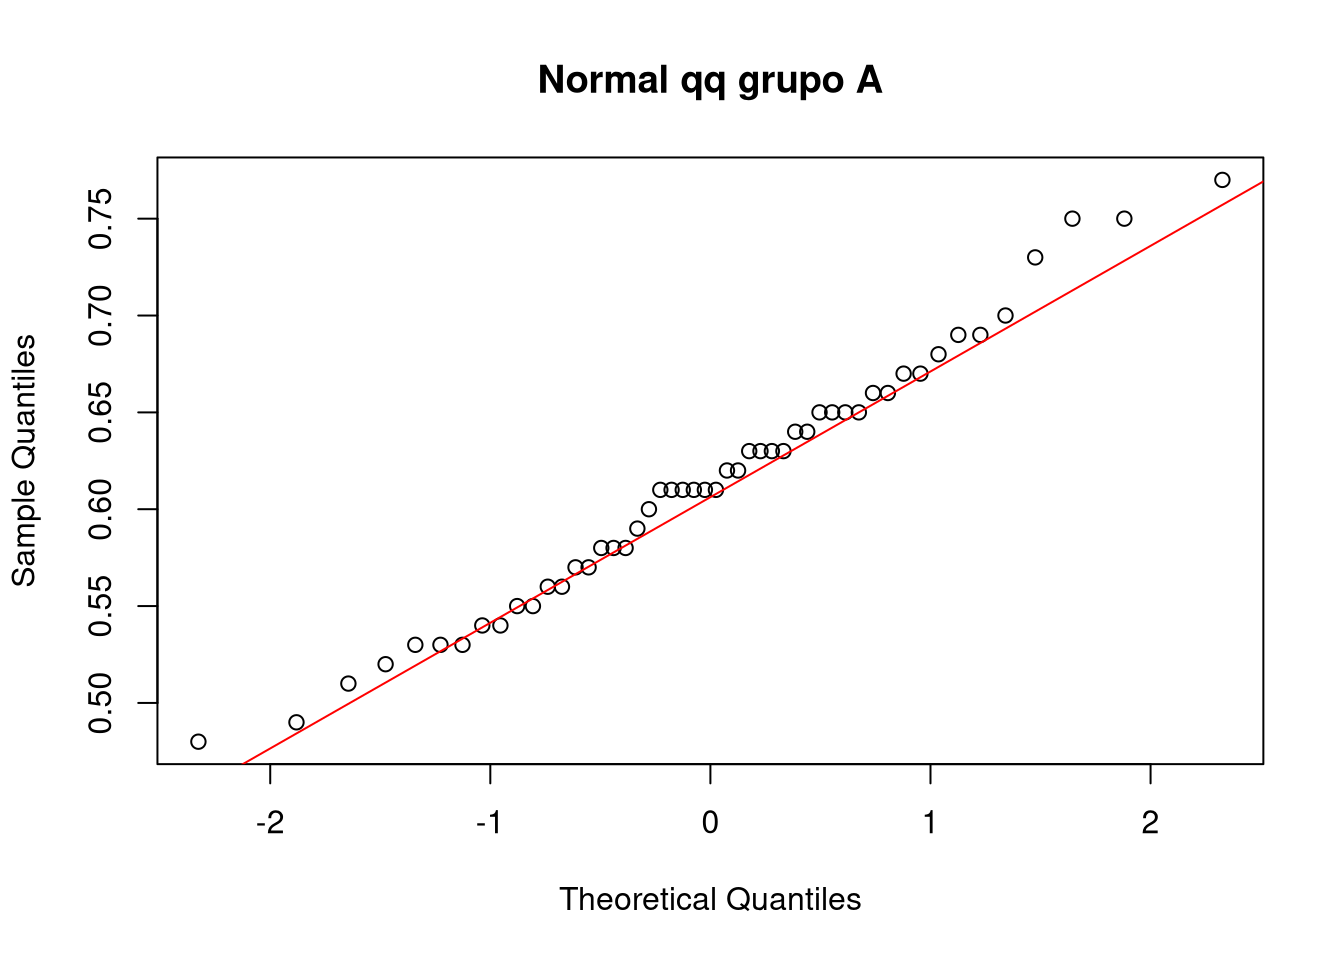
\includegraphics{Practica1_files/figure-latex/unnamed-chunk-15-4.pdf} *
¿Le parece a partir de estos datos que ambos grupos están midiendo lo
mismo?

\begin{Shaded}
\begin{Highlighting}[]
\NormalTok{centralidad }\OtherTok{=} \FunctionTok{matrix}\NormalTok{(}\AttributeTok{nrow =} \DecValTok{2}\NormalTok{,}\AttributeTok{ncol =} \DecValTok{4}\NormalTok{)}
\NormalTok{centralidad[}\DecValTok{1}\NormalTok{,}\DecValTok{1}\NormalTok{] }\OtherTok{=} \FunctionTok{mean}\NormalTok{(est}\SpecialCharTok{$}\NormalTok{GRUPO1)}
\NormalTok{centralidad[}\DecValTok{2}\NormalTok{,}\DecValTok{1}\NormalTok{] }\OtherTok{=} \FunctionTok{mean}\NormalTok{(est}\SpecialCharTok{$}\NormalTok{GRUPO2)}
\NormalTok{centralidad[}\DecValTok{1}\NormalTok{,}\DecValTok{2}\NormalTok{] }\OtherTok{=} \FunctionTok{median}\NormalTok{(est}\SpecialCharTok{$}\NormalTok{GRUPO1)}
\NormalTok{centralidad[}\DecValTok{2}\NormalTok{,}\DecValTok{2}\NormalTok{] }\OtherTok{=} \FunctionTok{median}\NormalTok{(est}\SpecialCharTok{$}\NormalTok{GRUPO2)}
\NormalTok{centralidad[}\DecValTok{1}\NormalTok{,}\DecValTok{3}\NormalTok{] }\OtherTok{=} \FunctionTok{mean}\NormalTok{(est}\SpecialCharTok{$}\NormalTok{GRUPO1,}\AttributeTok{trim =} \FloatTok{0.2}\NormalTok{)}
\NormalTok{centralidad[}\DecValTok{2}\NormalTok{,}\DecValTok{3}\NormalTok{] }\OtherTok{=} \FunctionTok{mean}\NormalTok{(est}\SpecialCharTok{$}\NormalTok{GRUPO2,}\AttributeTok{trim =} \FloatTok{0.2}\NormalTok{)}
\NormalTok{centralidad[}\DecValTok{1}\NormalTok{,}\DecValTok{4}\NormalTok{] }\OtherTok{=} \FunctionTok{mad}\NormalTok{(est}\SpecialCharTok{$}\NormalTok{GRUPO1)}
\NormalTok{centralidad[}\DecValTok{2}\NormalTok{,}\DecValTok{4}\NormalTok{] }\OtherTok{=} \FunctionTok{mad}\NormalTok{(est}\SpecialCharTok{$}\NormalTok{GRUPO2)}
\NormalTok{centralidad }\OtherTok{=} \FunctionTok{as.table}\NormalTok{(centralidad) }
\FunctionTok{rownames}\NormalTok{(centralidad) }\OtherTok{=} \FunctionTok{c}\NormalTok{(}\StringTok{"Grupo 1"}\NormalTok{,}\StringTok{"Grupo 2"}\NormalTok{)}
\FunctionTok{colnames}\NormalTok{(centralidad) }\OtherTok{=} \FunctionTok{c}\NormalTok{(}\StringTok{"media"}\NormalTok{, }\StringTok{"mediana"}\NormalTok{, }\StringTok{"{-}0.2 podada"}\NormalTok{, }\StringTok{"MAD"}\NormalTok{)}
\NormalTok{centralidad}
\end{Highlighting}
\end{Shaded}

\begin{verbatim}
##            media  mediana -0.2 podada      MAD
## Grupo 1 0.500000 0.500000    0.501000 0.014826
## Grupo 2 0.613600 0.610000    0.612000 0.066717
\end{verbatim}

Algo parecido se puede hacer con medidas de dispersion pero se
graficamente.

\begin{Shaded}
\begin{Highlighting}[]
\FunctionTok{boxplot}\NormalTok{(est}\SpecialCharTok{$}\NormalTok{GRUPO1,est}\SpecialCharTok{$}\NormalTok{GRUPO2,}\AttributeTok{main=} \StringTok{"Grupo 1 y Grupo 2"}\NormalTok{, }\AttributeTok{col =} \FunctionTok{c}\NormalTok{(}\StringTok{"red"}\NormalTok{,}\StringTok{"green"}\NormalTok{))}
\end{Highlighting}
\end{Shaded}

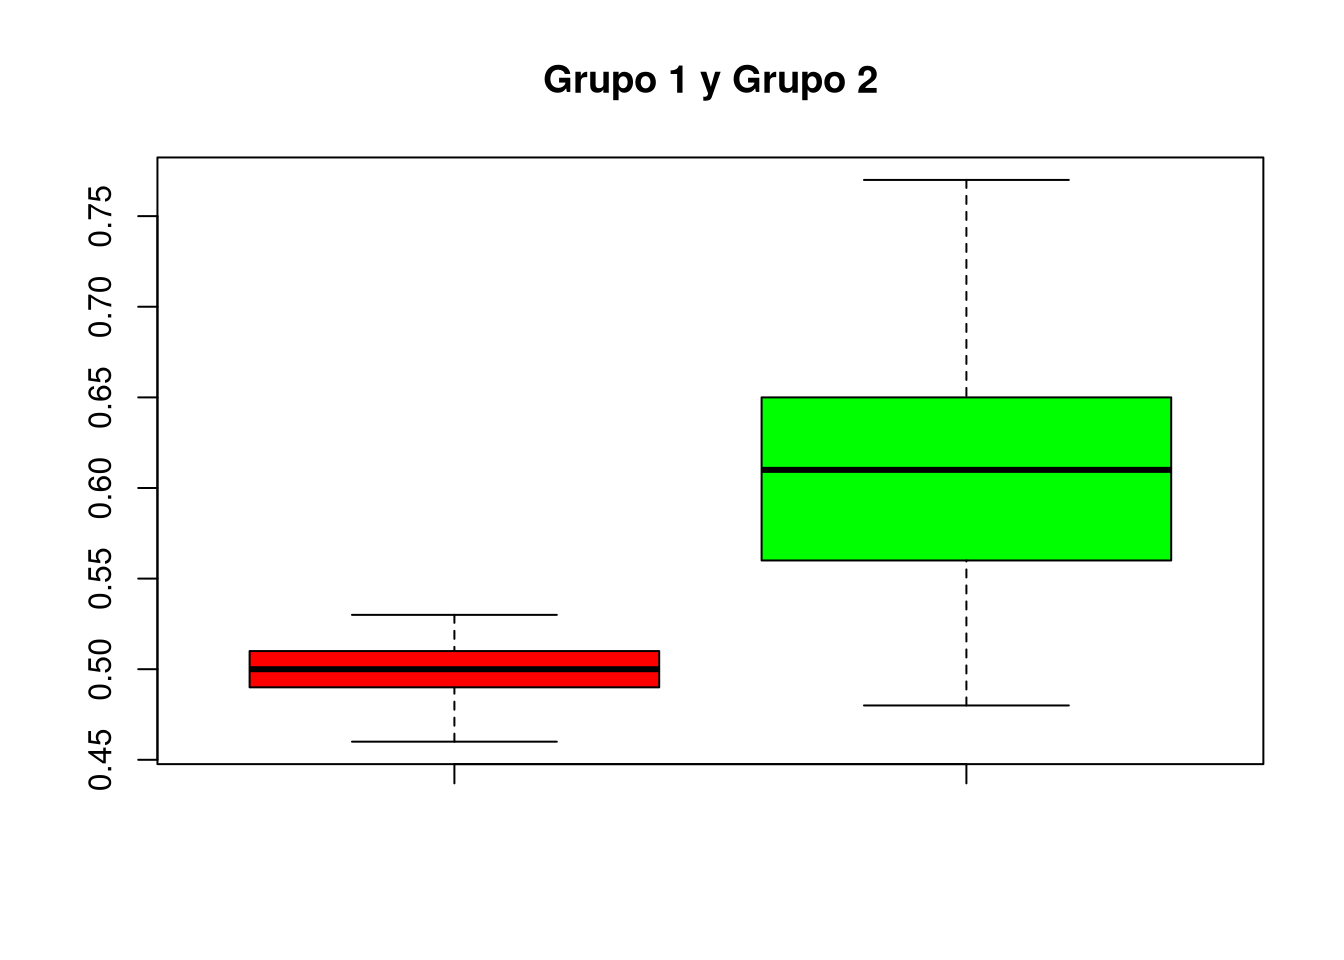
\includegraphics{Practica1_files/figure-latex/unnamed-chunk-17-1.pdf}
Parecen estar midiendo cosas distintas, ya que las medidas de dispersion
difieren por mucho, y algo parecido pasa con las medidas de centralidad.
****

\hypertarget{ejericio-6}{%
\section{EJericio 6:}\label{ejericio-6}}

\begin{itemize}
\tightlist
\item
\end{itemize}

\begin{Shaded}
\begin{Highlighting}[]
\CommentTok{\#cargamos los datos }
\FunctionTok{setwd}\NormalTok{(}\StringTok{"\textasciitilde{}/Documents/FCEyN/Estadistica/Datos"}\NormalTok{)}
\NormalTok{nubes }\OtherTok{=} \FunctionTok{read.table}\NormalTok{(}\StringTok{"nubes.txt"}\NormalTok{,}\AttributeTok{header=}\ConstantTok{TRUE}\NormalTok{)}
\end{Highlighting}
\end{Shaded}

\begin{itemize}
\item
  Realizar boxplots paralelos. ¿Le parece que el método produce algún
  efecto? \textgreater{} Parece haber mas outliyers favorables.
\item
  Realizar boxplots paralelos habiendo transformado las variables con el
  logaritmo natural. Observar cómo se modificaron los datos atı́picos
  respecto del ı́tem a). \textgreater{} Los outliyers parecen haberse
  ``normalizados''
\end{itemize}

\begin{Shaded}
\begin{Highlighting}[]
\NormalTok{tratadas }\OtherTok{=}\NormalTok{ nubes}\SpecialCharTok{$}\NormalTok{TRATADAS}
\NormalTok{controles }\OtherTok{=}\NormalTok{ nubes}\SpecialCharTok{$}\NormalTok{CONTROLES}
\NormalTok{nubs\_trat\_ln }\OtherTok{=} \FunctionTok{log}\NormalTok{(tratadas)}
\NormalTok{nubs\_contr\_ln }\OtherTok{=} \FunctionTok{log}\NormalTok{(controles)}
\FunctionTok{boxplot}\NormalTok{(tratadas, controles, }\AttributeTok{main =}\StringTok{"Nubes tratadas y controles"}\NormalTok{)}
\end{Highlighting}
\end{Shaded}

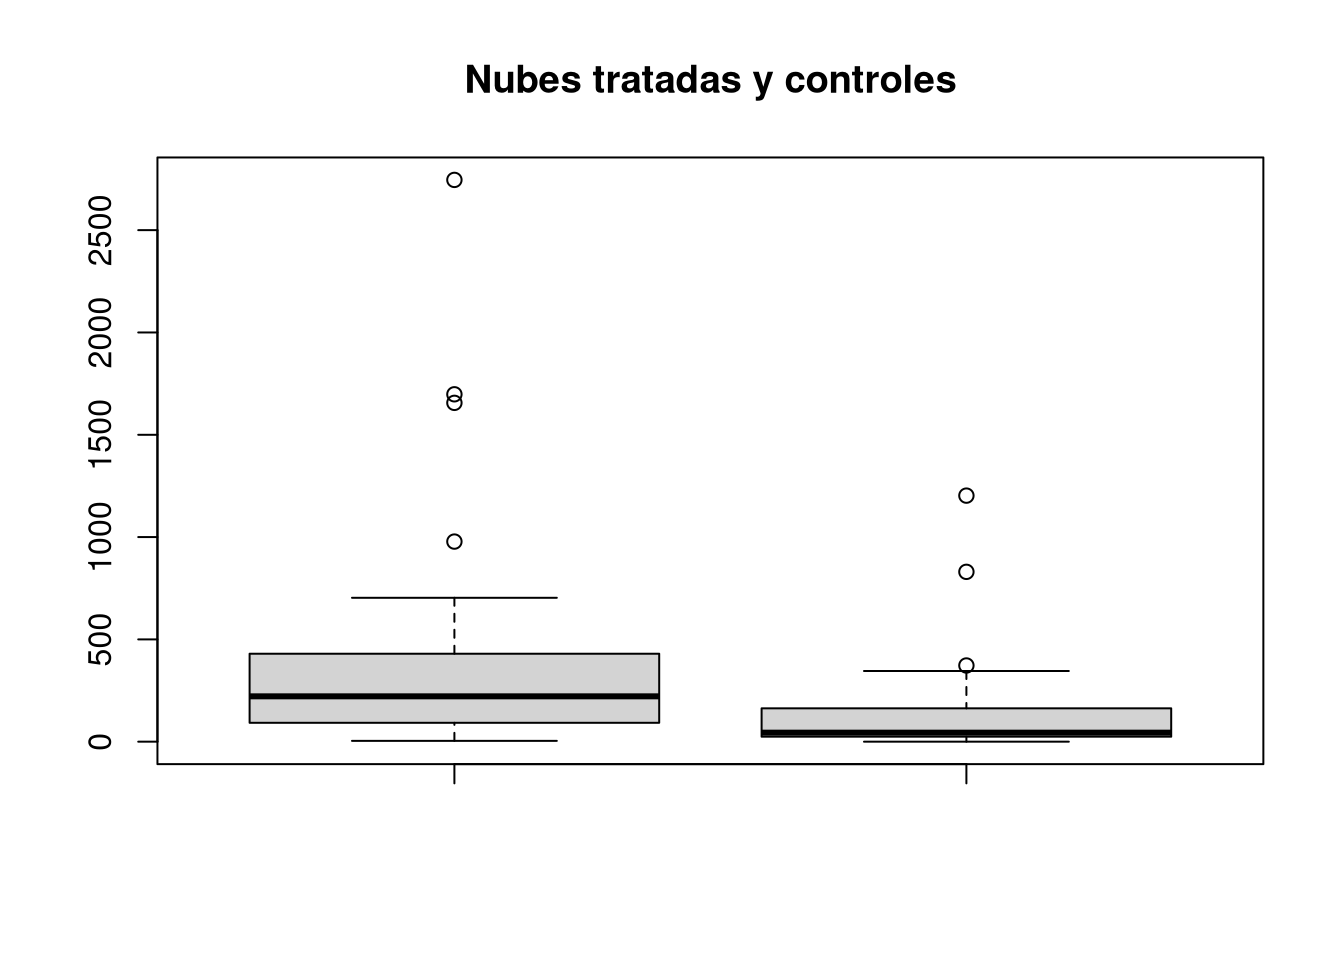
\includegraphics{Practica1_files/figure-latex/unnamed-chunk-19-1.pdf}

\begin{Shaded}
\begin{Highlighting}[]
\FunctionTok{boxplot}\NormalTok{(nubs\_trat\_ln,nubs\_contr\_ln, }\AttributeTok{main =} \StringTok{"ln(tratadas) y ln(controles)"}\NormalTok{)}
\end{Highlighting}
\end{Shaded}

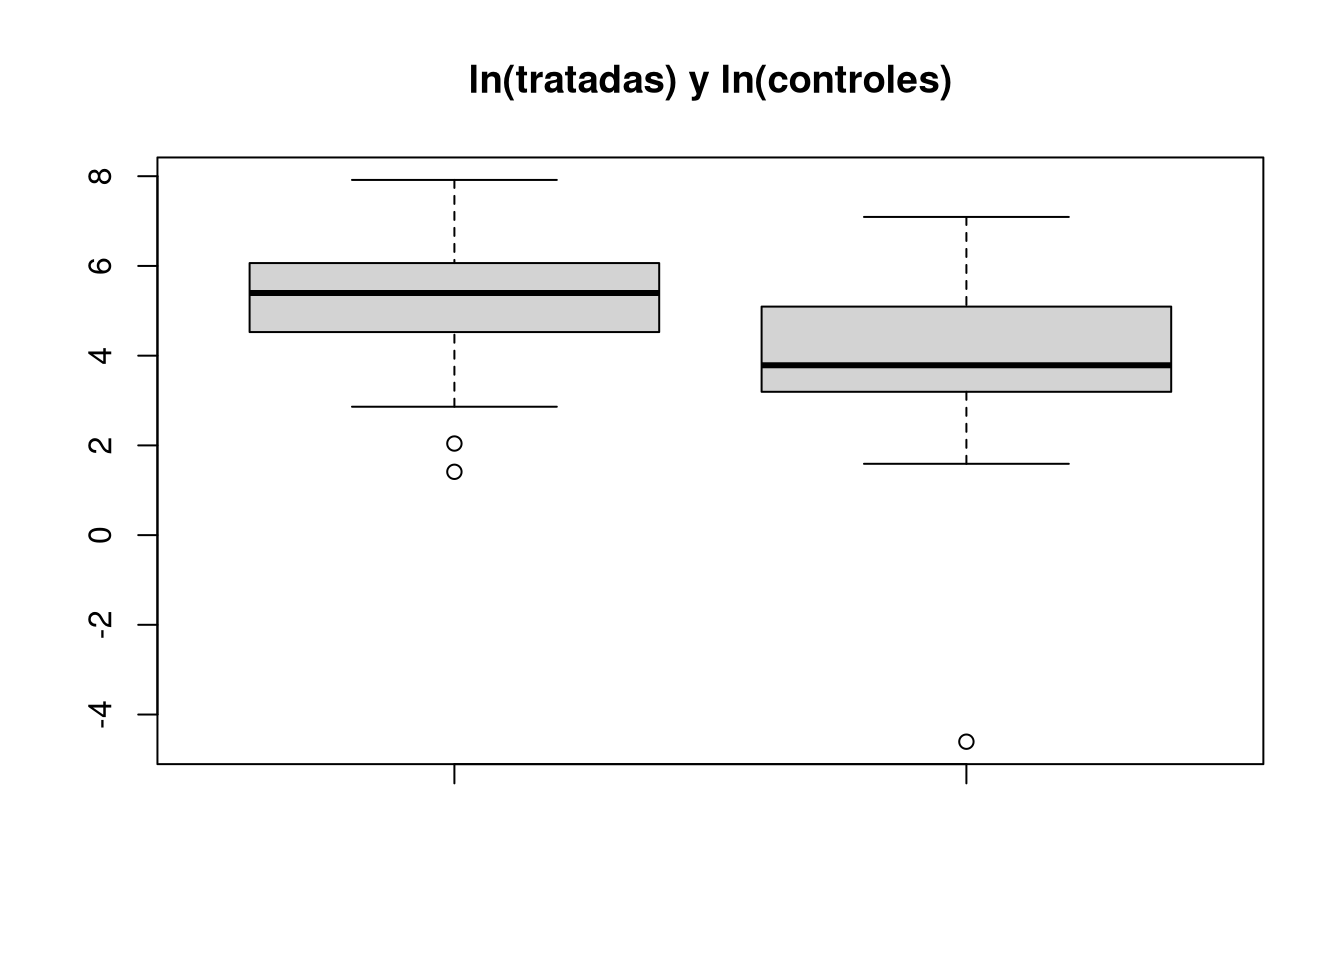
\includegraphics{Practica1_files/figure-latex/unnamed-chunk-19-2.pdf} *
Analizar la normalidad realizando qqplots e histogramas (de densidad)
para ambos conjuntos de datos y superponiendo la curva normal
\textgreater{} Concluyo que ambas distribuciones no parecen venir de una
normal.

\begin{Shaded}
\begin{Highlighting}[]
\FunctionTok{hist}\NormalTok{(tratadas,}\AttributeTok{freq =} \ConstantTok{FALSE}\NormalTok{, }\AttributeTok{main =} \StringTok{"Histograma de nubes tratadas"}\NormalTok{)}
\FunctionTok{lines}\NormalTok{(}\FunctionTok{density}\NormalTok{(tratadas)) }\CommentTok{\# Recordar que es una aproximacion a la densidad, por el nucleo normal por defecto (creo)}
\FunctionTok{grid}\NormalTok{(}\AttributeTok{nx =} \ConstantTok{NA}\NormalTok{, }\AttributeTok{ny =} \ConstantTok{NULL}\NormalTok{, }\AttributeTok{lty =} \DecValTok{2}\NormalTok{, }\AttributeTok{col =} \StringTok{"gray"}\NormalTok{, }\AttributeTok{lwd =} \DecValTok{1}\NormalTok{)}
\end{Highlighting}
\end{Shaded}

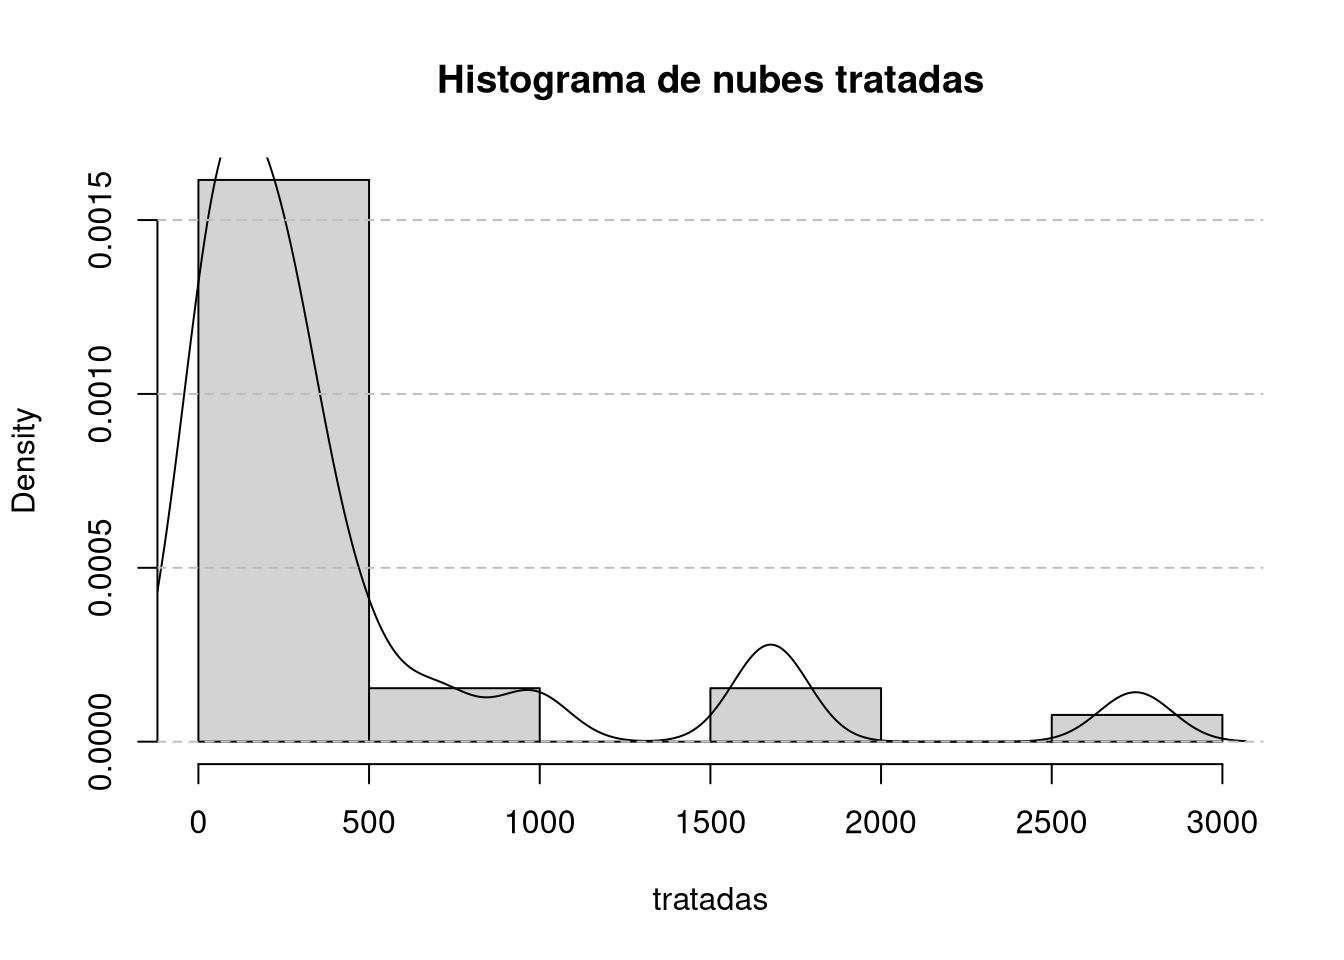
\includegraphics{Practica1_files/figure-latex/unnamed-chunk-20-1.pdf}

\begin{Shaded}
\begin{Highlighting}[]
\FunctionTok{qqnorm}\NormalTok{(tratadas,}\AttributeTok{main=}\StringTok{"Normal Q{-}Q Nubes tratadas"}\NormalTok{)}
\FunctionTok{qqline}\NormalTok{(tratadas,}\AttributeTok{col =} \StringTok{"red"}\NormalTok{)}
\end{Highlighting}
\end{Shaded}

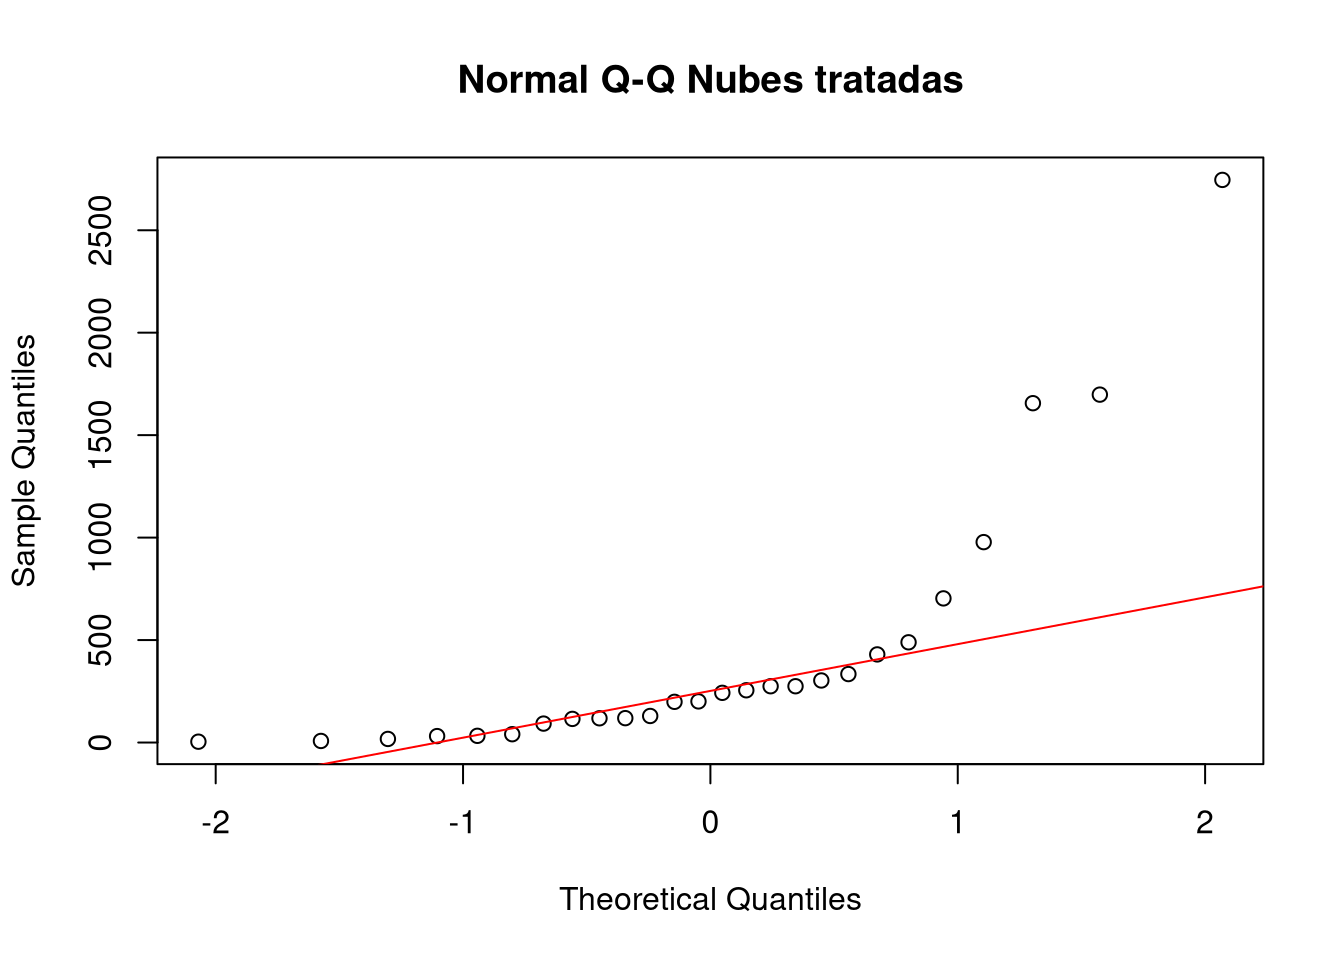
\includegraphics{Practica1_files/figure-latex/unnamed-chunk-20-2.pdf}

\begin{Shaded}
\begin{Highlighting}[]
\FunctionTok{hist}\NormalTok{(controles,}\AttributeTok{freq =} \ConstantTok{FALSE}\NormalTok{)}
\FunctionTok{lines}\NormalTok{(}\FunctionTok{density}\NormalTok{(controles)) }\CommentTok{\# Recordar que es una aproximacion a la densidad, por el nucleo normal por defecto (creo)}
\FunctionTok{grid}\NormalTok{(}\AttributeTok{nx =} \ConstantTok{NA}\NormalTok{, }\AttributeTok{ny =} \ConstantTok{NULL}\NormalTok{, }\AttributeTok{lty =} \DecValTok{2}\NormalTok{, }\AttributeTok{col =} \StringTok{"gray"}\NormalTok{, }\AttributeTok{lwd =} \DecValTok{1}\NormalTok{)}
\end{Highlighting}
\end{Shaded}

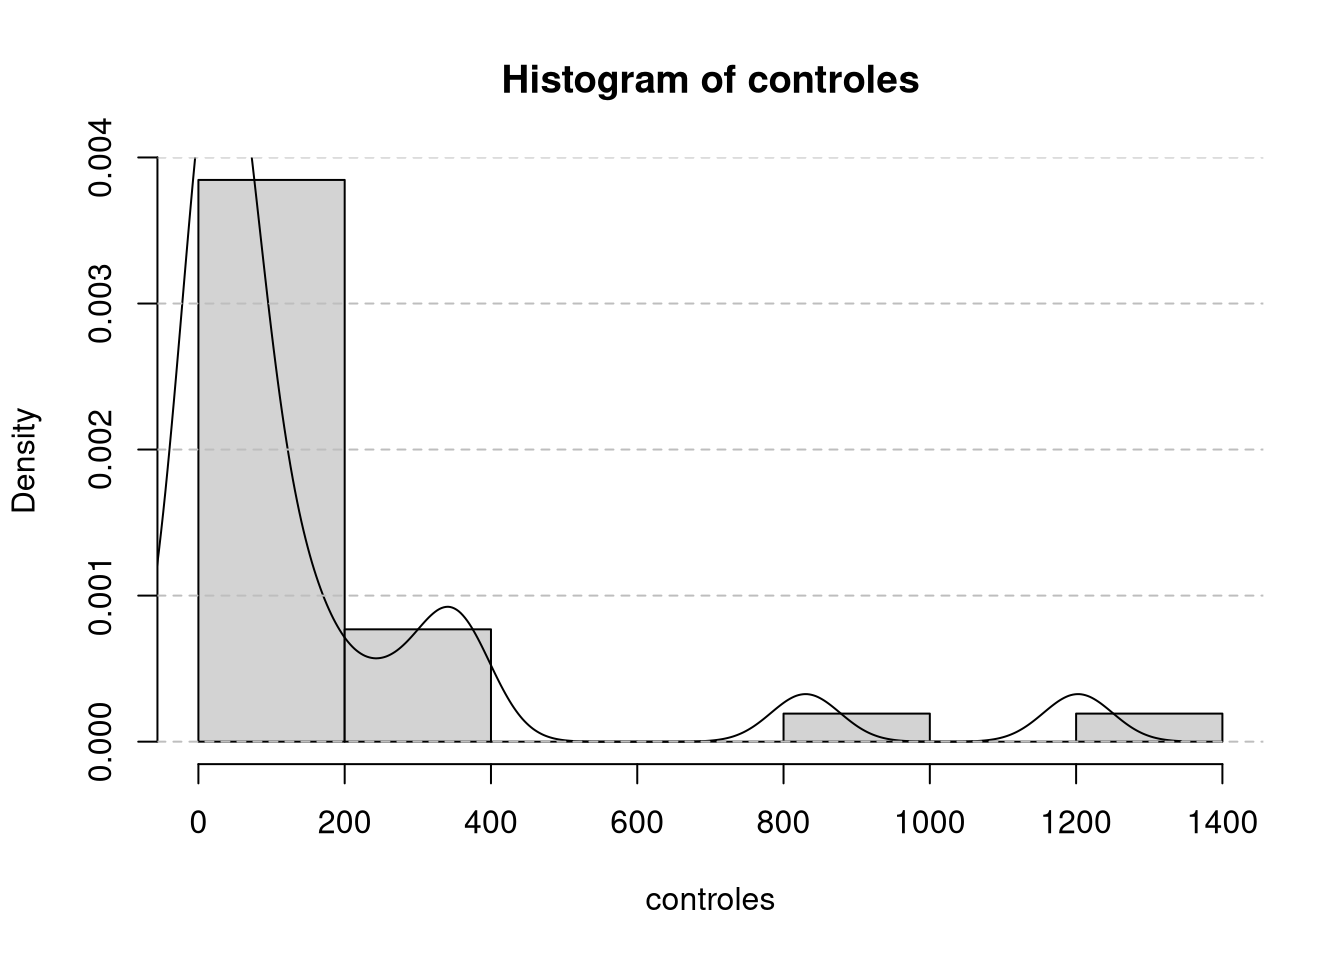
\includegraphics{Practica1_files/figure-latex/unnamed-chunk-20-3.pdf}

\begin{Shaded}
\begin{Highlighting}[]
\FunctionTok{qqnorm}\NormalTok{(controles,}\AttributeTok{main=}\StringTok{"Normal Q{-}Q Nubes controles"}\NormalTok{)}
\FunctionTok{qqline}\NormalTok{(controles,}\AttributeTok{col =} \StringTok{"red"}\NormalTok{)}
\end{Highlighting}
\end{Shaded}

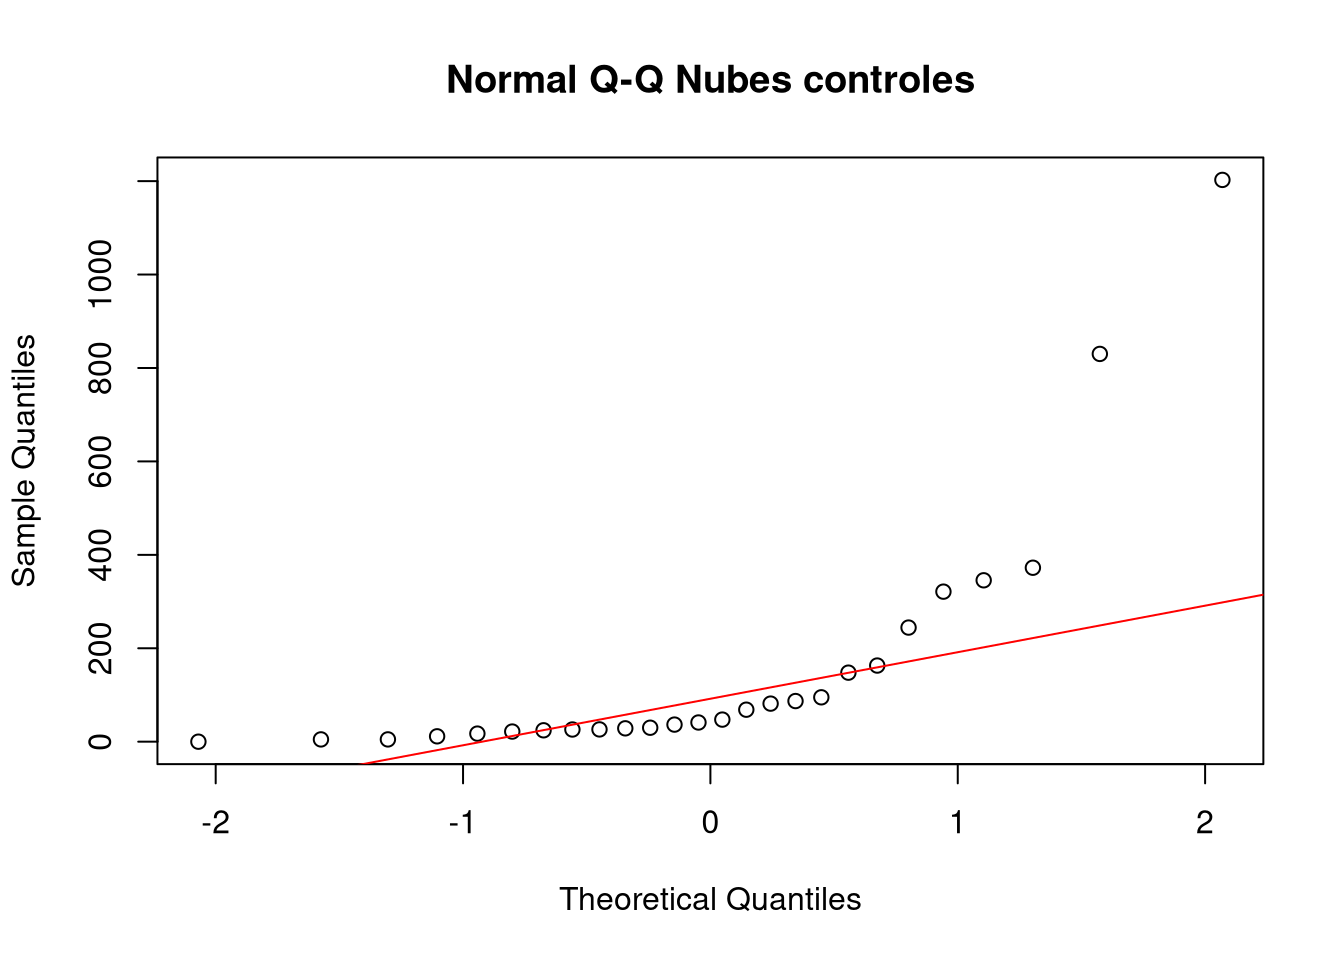
\includegraphics{Practica1_files/figure-latex/unnamed-chunk-20-4.pdf}

\begin{itemize}
\tightlist
\item
  Realizar la transformación logaritmo natural a los datos (log en R) y
  repetir b) para los datos transformados. \textgreater{} Para las
  controles si no fuese por un dato atipico puede asemejarse a una
  normal.
\end{itemize}

\begin{Shaded}
\begin{Highlighting}[]
\CommentTok{\#Analizamos normalidad de los datos }

\FunctionTok{hist}\NormalTok{(nubs\_trat\_ln,}\AttributeTok{freq =} \ConstantTok{FALSE}\NormalTok{, }\AttributeTok{main =} \StringTok{"Histograma de ln(tratadas)"}\NormalTok{)}
\FunctionTok{lines}\NormalTok{(}\FunctionTok{density}\NormalTok{(nubs\_trat\_ln)) }\CommentTok{\# Recordar que es una aproximacion a la densidad, por el nucleo normal por defecto (creo)}
\FunctionTok{grid}\NormalTok{(}\AttributeTok{nx =} \ConstantTok{NA}\NormalTok{, }\AttributeTok{ny =} \ConstantTok{NULL}\NormalTok{, }\AttributeTok{lty =} \DecValTok{2}\NormalTok{, }\AttributeTok{col =} \StringTok{"gray"}\NormalTok{, }\AttributeTok{lwd =} \DecValTok{1}\NormalTok{)}
\end{Highlighting}
\end{Shaded}

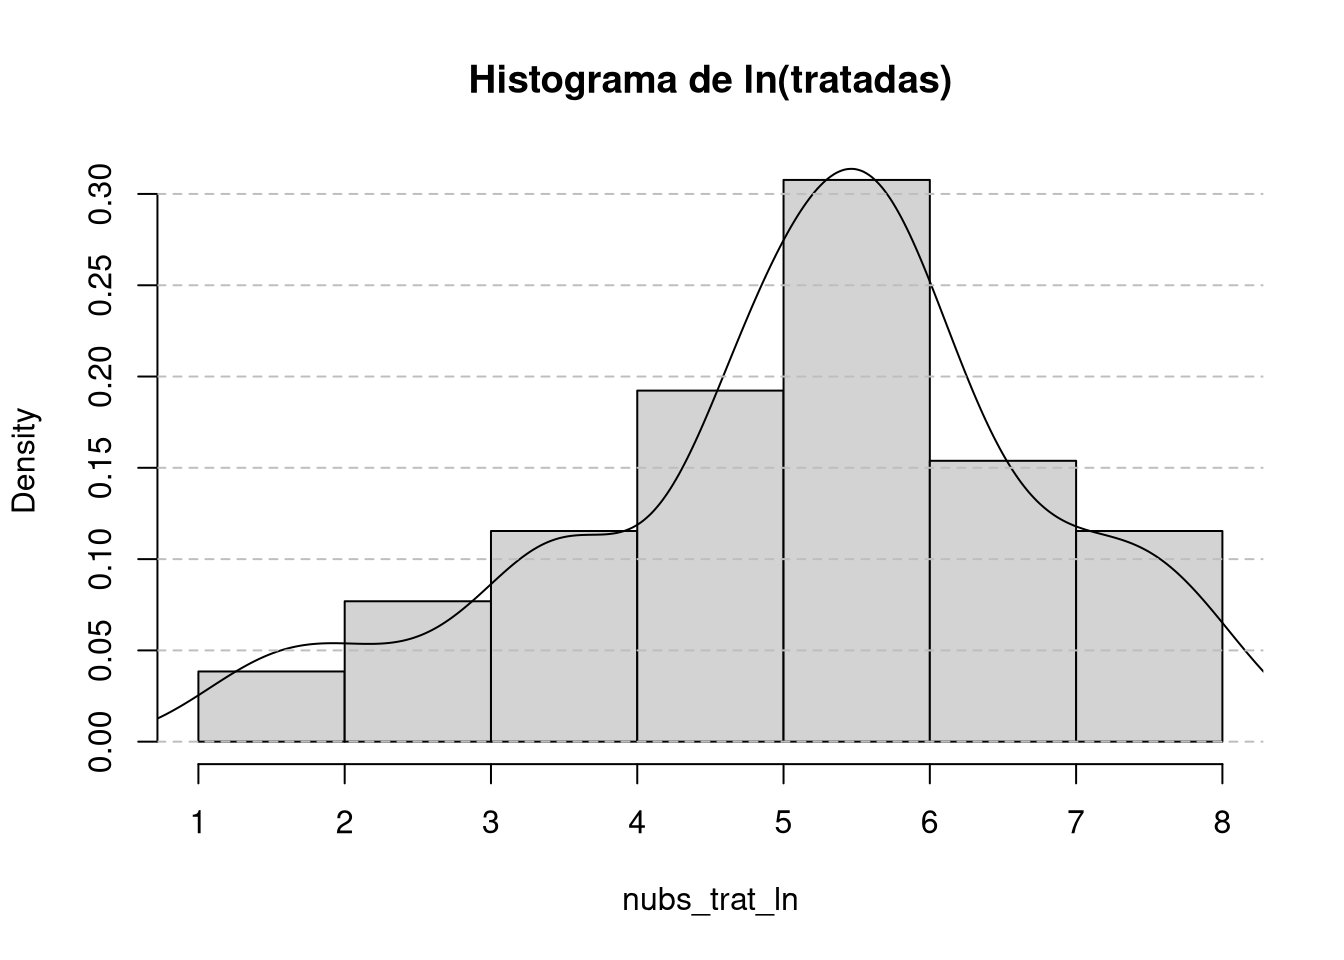
\includegraphics{Practica1_files/figure-latex/unnamed-chunk-21-1.pdf}

\begin{Shaded}
\begin{Highlighting}[]
\FunctionTok{qqnorm}\NormalTok{(nubs\_trat\_ln,}\AttributeTok{main=}\StringTok{"Normal Q{-}Q ln(tratadas)"}\NormalTok{)}
\FunctionTok{qqline}\NormalTok{(nubs\_trat\_ln,}\AttributeTok{col =} \StringTok{"red"}\NormalTok{)}
\end{Highlighting}
\end{Shaded}

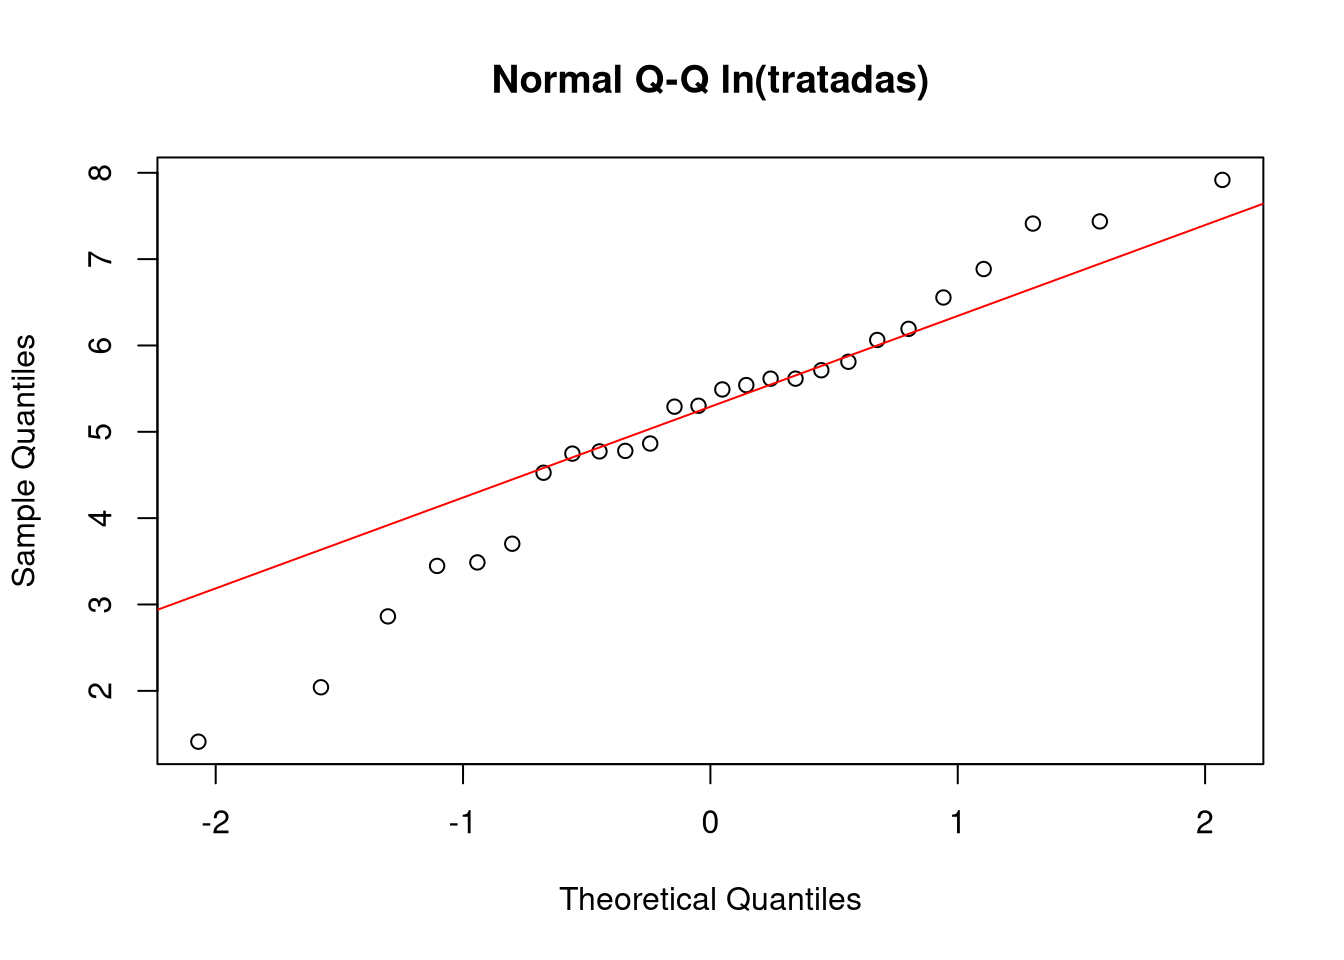
\includegraphics{Practica1_files/figure-latex/unnamed-chunk-21-2.pdf}

\begin{Shaded}
\begin{Highlighting}[]
\FunctionTok{hist}\NormalTok{(nubs\_contr\_ln,}\AttributeTok{freq =} \ConstantTok{FALSE}\NormalTok{, }\AttributeTok{main =} \StringTok{"Histograma de ln(controles)"}\NormalTok{)}
\FunctionTok{lines}\NormalTok{(}\FunctionTok{density}\NormalTok{(nubs\_contr\_ln)) }\CommentTok{\# Recordar que es una aproximacion a la densidad, por el nucleo normal por defecto (creo)}
\FunctionTok{grid}\NormalTok{(}\AttributeTok{nx =} \ConstantTok{NA}\NormalTok{, }\AttributeTok{ny =} \ConstantTok{NULL}\NormalTok{, }\AttributeTok{lty =} \DecValTok{2}\NormalTok{, }\AttributeTok{col =} \StringTok{"gray"}\NormalTok{, }\AttributeTok{lwd =} \DecValTok{1}\NormalTok{)}
\end{Highlighting}
\end{Shaded}

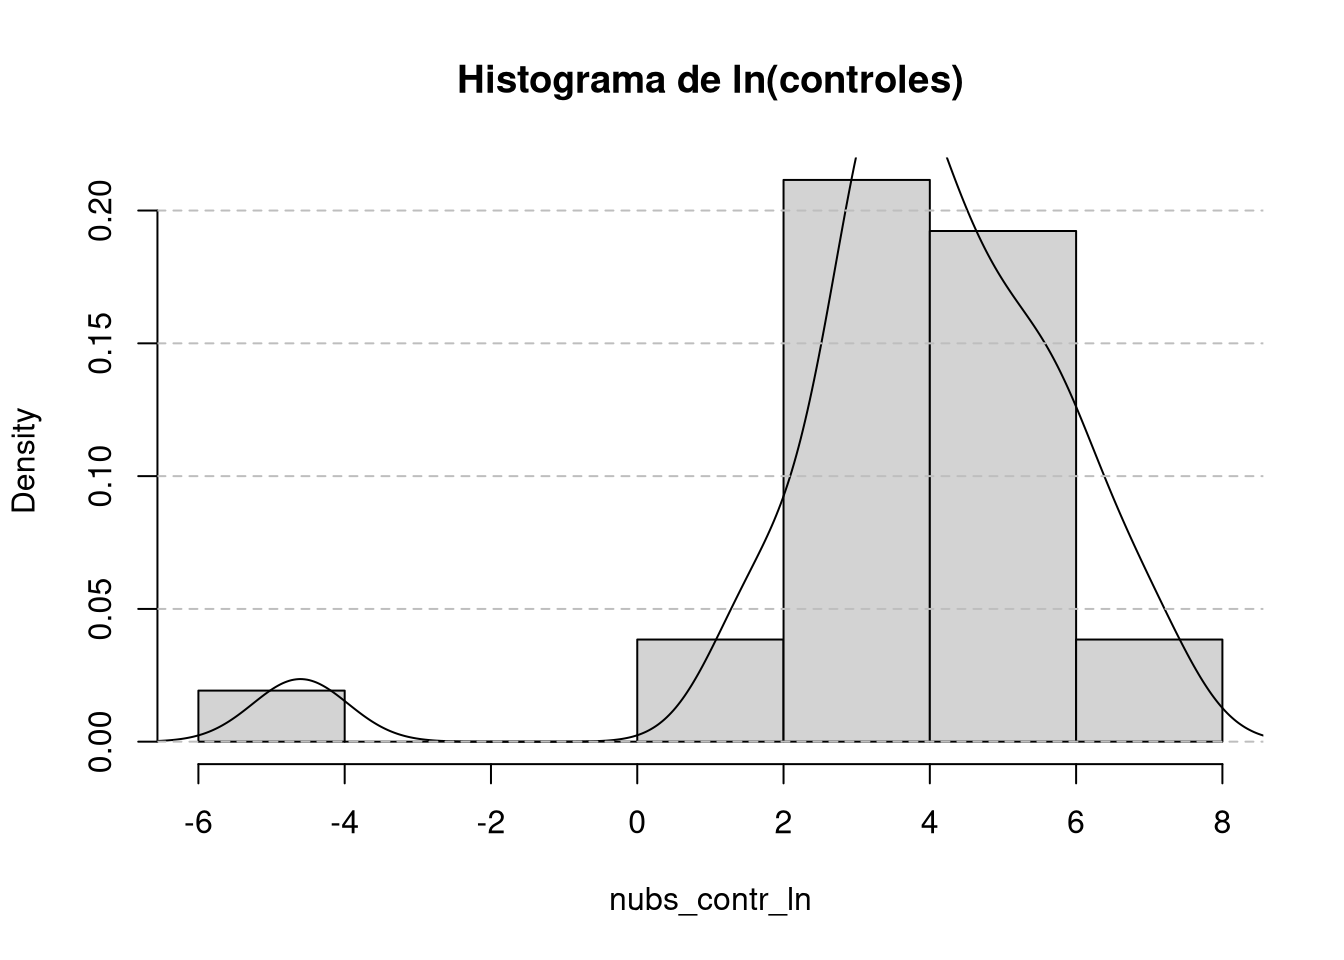
\includegraphics{Practica1_files/figure-latex/unnamed-chunk-21-3.pdf}

\begin{Shaded}
\begin{Highlighting}[]
\FunctionTok{qqnorm}\NormalTok{(nubs\_contr\_ln,}\AttributeTok{main=}\StringTok{"Normal Q{-}Q ln(controles)"}\NormalTok{)}
\FunctionTok{qqline}\NormalTok{(nubs\_contr\_ln,}\AttributeTok{col =} \StringTok{"red"}\NormalTok{)}
\end{Highlighting}
\end{Shaded}

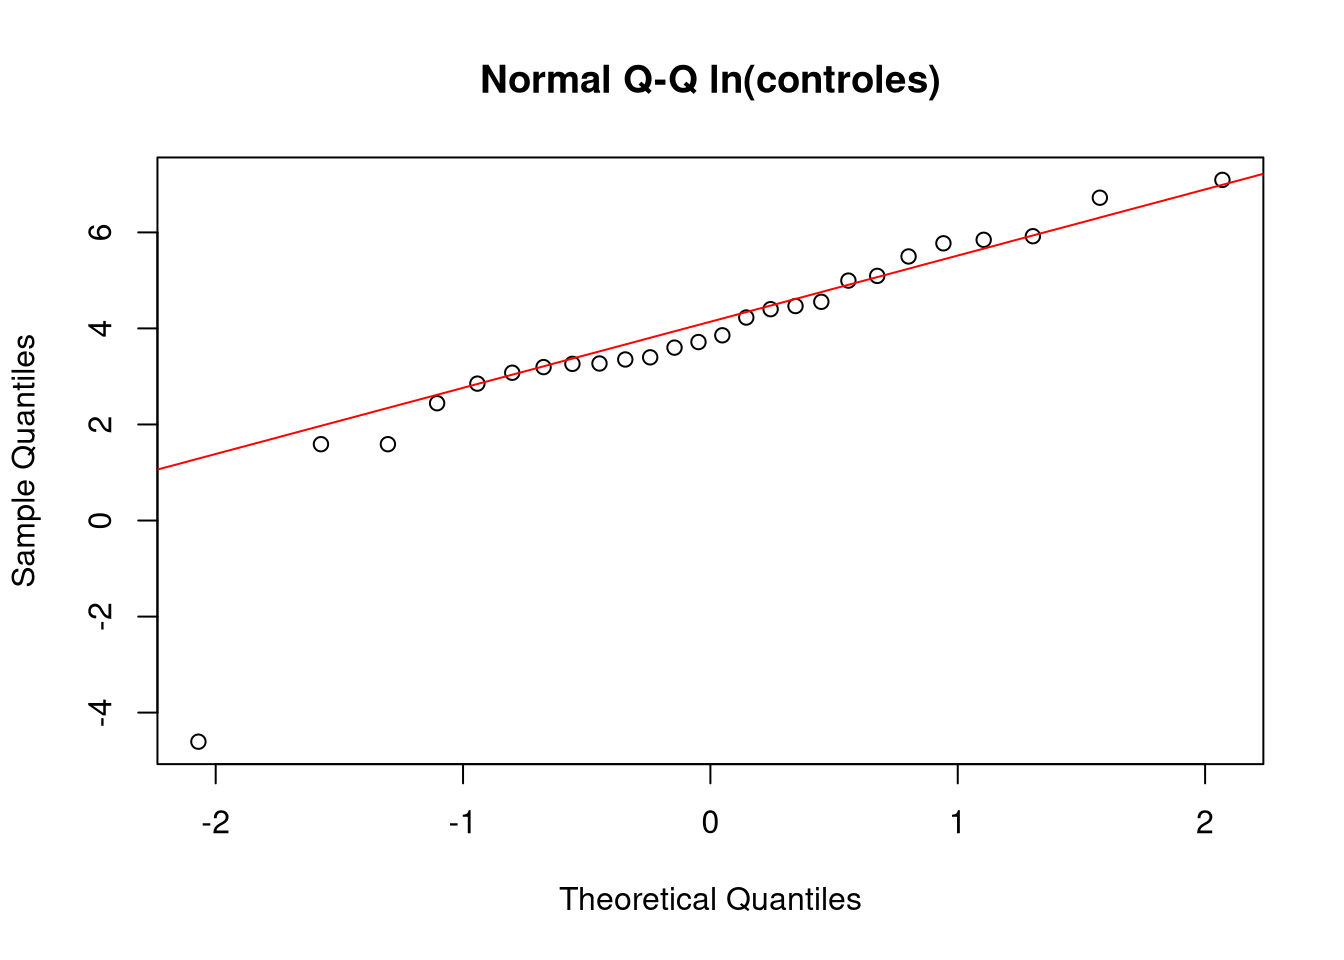
\includegraphics{Practica1_files/figure-latex/unnamed-chunk-21-4.pdf}

\begin{verbatim}
                                                            ****
\end{verbatim}

\hypertarget{ejericio-7}{%
\section{EJericio 7:}\label{ejericio-7}}

\begin{Shaded}
\begin{Highlighting}[]
\FunctionTok{setwd}\NormalTok{(}\StringTok{"\textasciitilde{}/Documents/FCEyN/Estadistica/Datos"}\NormalTok{)}
\NormalTok{cpu }\OtherTok{=} \FunctionTok{read.table}\NormalTok{(}\StringTok{"cpu.txt"}\NormalTok{,}\AttributeTok{header =} \ConstantTok{TRUE}\NormalTok{)}
\NormalTok{cpu }\OtherTok{=}\NormalTok{ cpu}\SpecialCharTok{$}\NormalTok{X1}\FloatTok{.86}
\end{Highlighting}
\end{Shaded}

\begin{itemize}
\tightlist
\item
  Calcular la media muestral, la mediana muestral y la media α-podada
  muestral con α = 0,10 (10 \%)
\end{itemize}

\begin{Shaded}
\begin{Highlighting}[]
\NormalTok{m }\OtherTok{=} \FunctionTok{matrix}\NormalTok{(}\AttributeTok{ncol =} \DecValTok{3}\NormalTok{,}\AttributeTok{nrow =} \DecValTok{1}\NormalTok{)}
\NormalTok{m[}\DecValTok{1}\NormalTok{,}\DecValTok{1}\NormalTok{] }\OtherTok{=} \FunctionTok{mean}\NormalTok{(cpu)}
\NormalTok{m[}\DecValTok{1}\NormalTok{,}\DecValTok{2}\NormalTok{] }\OtherTok{=} \FunctionTok{median}\NormalTok{(cpu)}
\NormalTok{m[}\DecValTok{1}\NormalTok{,}\DecValTok{3}\NormalTok{] }\OtherTok{=} \FunctionTok{mean}\NormalTok{(cpu, }\AttributeTok{trim =} \FloatTok{0.1}\NormalTok{)}
\NormalTok{m }\OtherTok{=} \FunctionTok{as.table}\NormalTok{(m)}
\FunctionTok{rownames}\NormalTok{(m) }\OtherTok{=} \FunctionTok{c}\NormalTok{(}\StringTok{"cpu"}\NormalTok{)}
\FunctionTok{colnames}\NormalTok{(m) }\OtherTok{=} \FunctionTok{c}\NormalTok{(}\StringTok{"media"}\NormalTok{,}\StringTok{"mediana"}\NormalTok{,}\StringTok{"media 0.1"}\NormalTok{)}
\NormalTok{m}
\end{Highlighting}
\end{Shaded}

\begin{verbatim}
##        media  mediana media 0.1
## cpu 4.751491 3.190000  3.929476
\end{verbatim}

\begin{itemize}
\tightlist
\item
  Calcular el desvı́o estándar, la distancia intercuartil y la MAD
  muestrales
\end{itemize}

\begin{Shaded}
\begin{Highlighting}[]
\NormalTok{u }\OtherTok{=} \FunctionTok{matrix}\NormalTok{(}\AttributeTok{nrow =} \DecValTok{1}\NormalTok{, }\AttributeTok{ncol =} \DecValTok{3}\NormalTok{)}
\NormalTok{u[}\DecValTok{1}\NormalTok{,}\DecValTok{1}\NormalTok{] }\OtherTok{=} \FunctionTok{sd}\NormalTok{(cpu)}
\NormalTok{u[}\DecValTok{1}\NormalTok{,}\DecValTok{2}\NormalTok{] }\OtherTok{=} \FunctionTok{IQR}\NormalTok{(cpu)}
\NormalTok{u[}\DecValTok{1}\NormalTok{,}\DecValTok{3}\NormalTok{] }\OtherTok{=} \FunctionTok{mad}\NormalTok{(cpu)}
\NormalTok{u }\OtherTok{=} \FunctionTok{as.table}\NormalTok{(u)}
\FunctionTok{rownames}\NormalTok{(u) }\OtherTok{=} \StringTok{"cpu"}
\FunctionTok{colnames}\NormalTok{(u) }\OtherTok{=} \FunctionTok{c}\NormalTok{(}\StringTok{"desvio estandar"}\NormalTok{,}\StringTok{"distancia intercuantil"}\NormalTok{,}\StringTok{"MAD"}\NormalTok{)}
\NormalTok{u}
\end{Highlighting}
\end{Shaded}

\begin{verbatim}
##     desvio estandar distancia intercuantil      MAD
## cpu        4.645589               4.475000 2.713158
\end{verbatim}

\begin{itemize}
\tightlist
\item
  Realizar un histograma, un gráfico de la densidad estimada usando la
  función density y un boxplot. ¿Cuáles son las caracterı́sticas más
  sobresalientes? ¿Se observan datos atı́picos? \textgreater{} Se
  observan bastantes datos atipicos y la densidad esta corrida a
  izquierda.
\end{itemize}

\begin{Shaded}
\begin{Highlighting}[]
\FunctionTok{hist}\NormalTok{(cpu, }\AttributeTok{freq =} \ConstantTok{FALSE}\NormalTok{, }\AttributeTok{main =} \StringTok{"Histograma de cpu"}\NormalTok{)}
\FunctionTok{lines}\NormalTok{(}\FunctionTok{density}\NormalTok{(cpu))}
\FunctionTok{grid}\NormalTok{(}\AttributeTok{nx =} \ConstantTok{NA}\NormalTok{, }\AttributeTok{ny =} \ConstantTok{NULL}\NormalTok{, }\AttributeTok{lty =} \DecValTok{2}\NormalTok{, }\AttributeTok{col =} \StringTok{"gray"}\NormalTok{, }\AttributeTok{lwd =} \DecValTok{1}\NormalTok{)}
\end{Highlighting}
\end{Shaded}

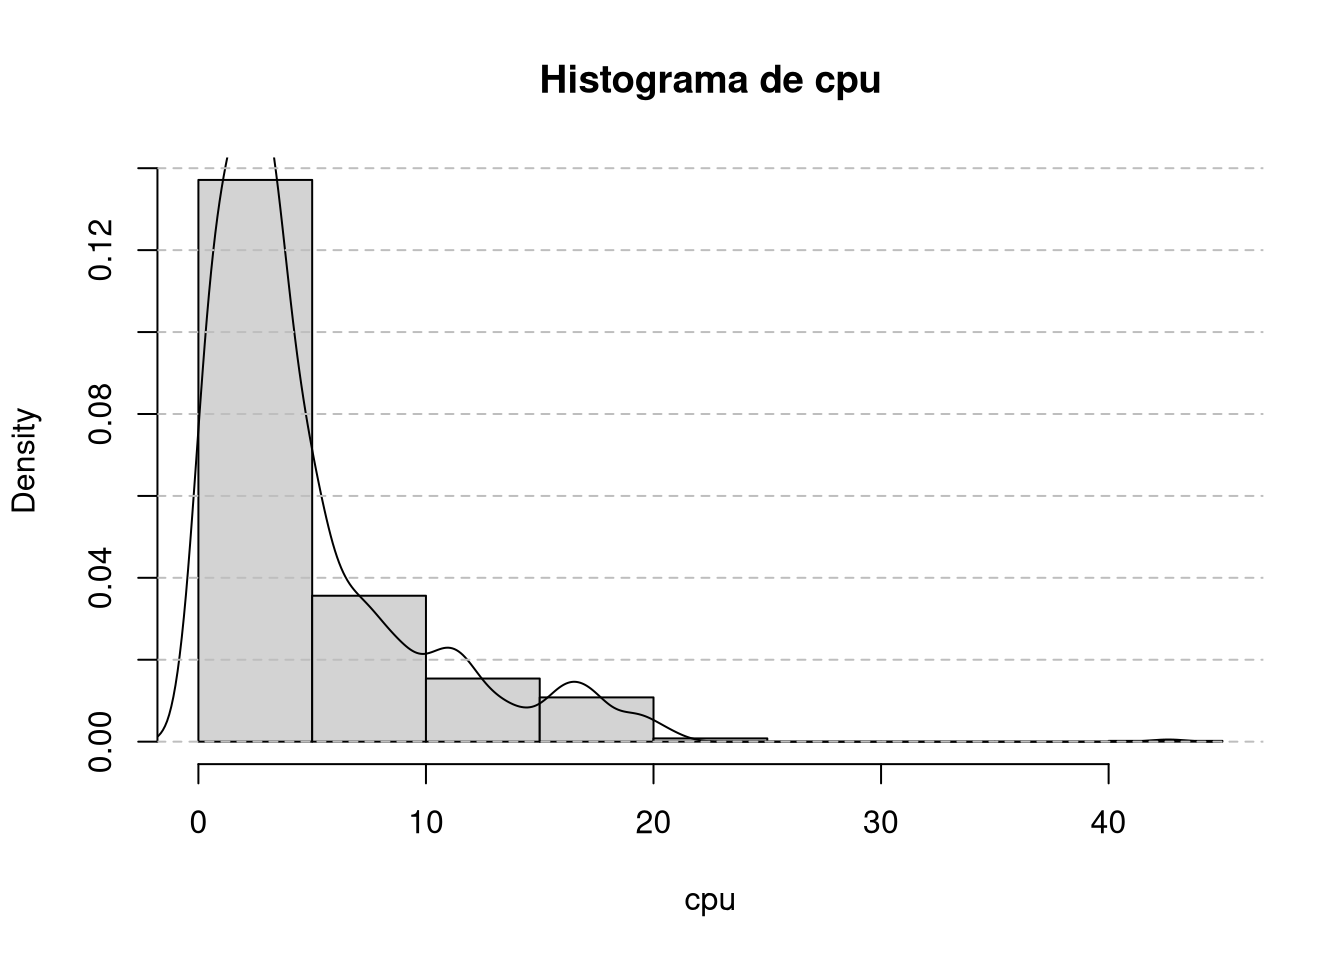
\includegraphics{Practica1_files/figure-latex/unnamed-chunk-25-1.pdf}

\begin{Shaded}
\begin{Highlighting}[]
\FunctionTok{boxplot}\NormalTok{(cpu)}
\end{Highlighting}
\end{Shaded}

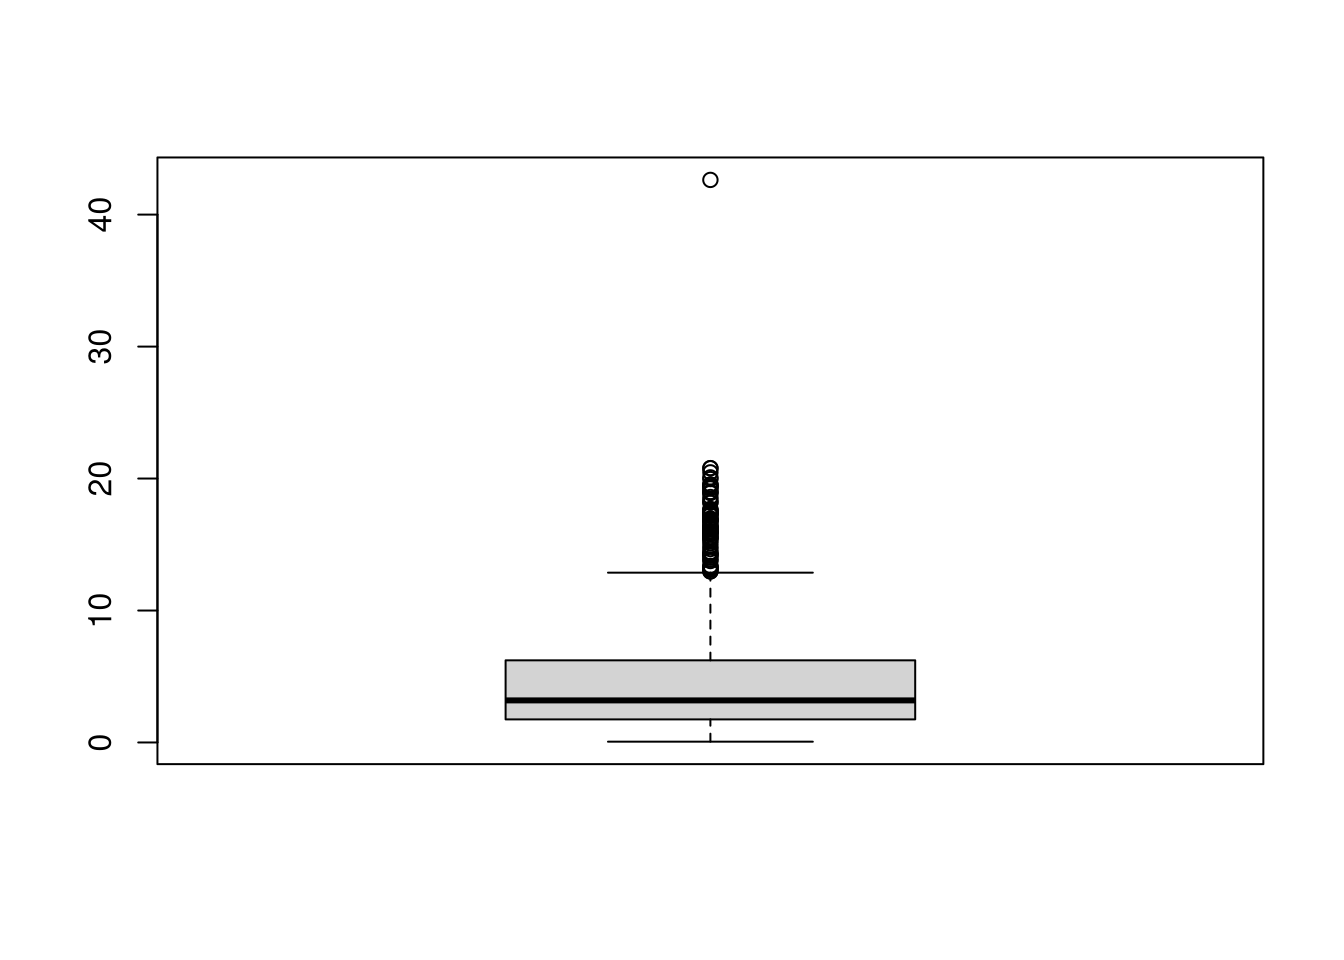
\includegraphics{Practica1_files/figure-latex/unnamed-chunk-25-2.pdf}

\begin{itemize}
\tightlist
\item
  ¿Cree que los datos tienen distribución normal? Hacer un qqplot para
  constatar su conjetura o ponerla en duda. \textgreater{} No parece
  tener una distribucion normal.
\end{itemize}

\begin{Shaded}
\begin{Highlighting}[]
\FunctionTok{qqnorm}\NormalTok{(cpu)}
\FunctionTok{qqline}\NormalTok{(cpu, }\AttributeTok{col =} \StringTok{"red"}\NormalTok{)}
\end{Highlighting}
\end{Shaded}

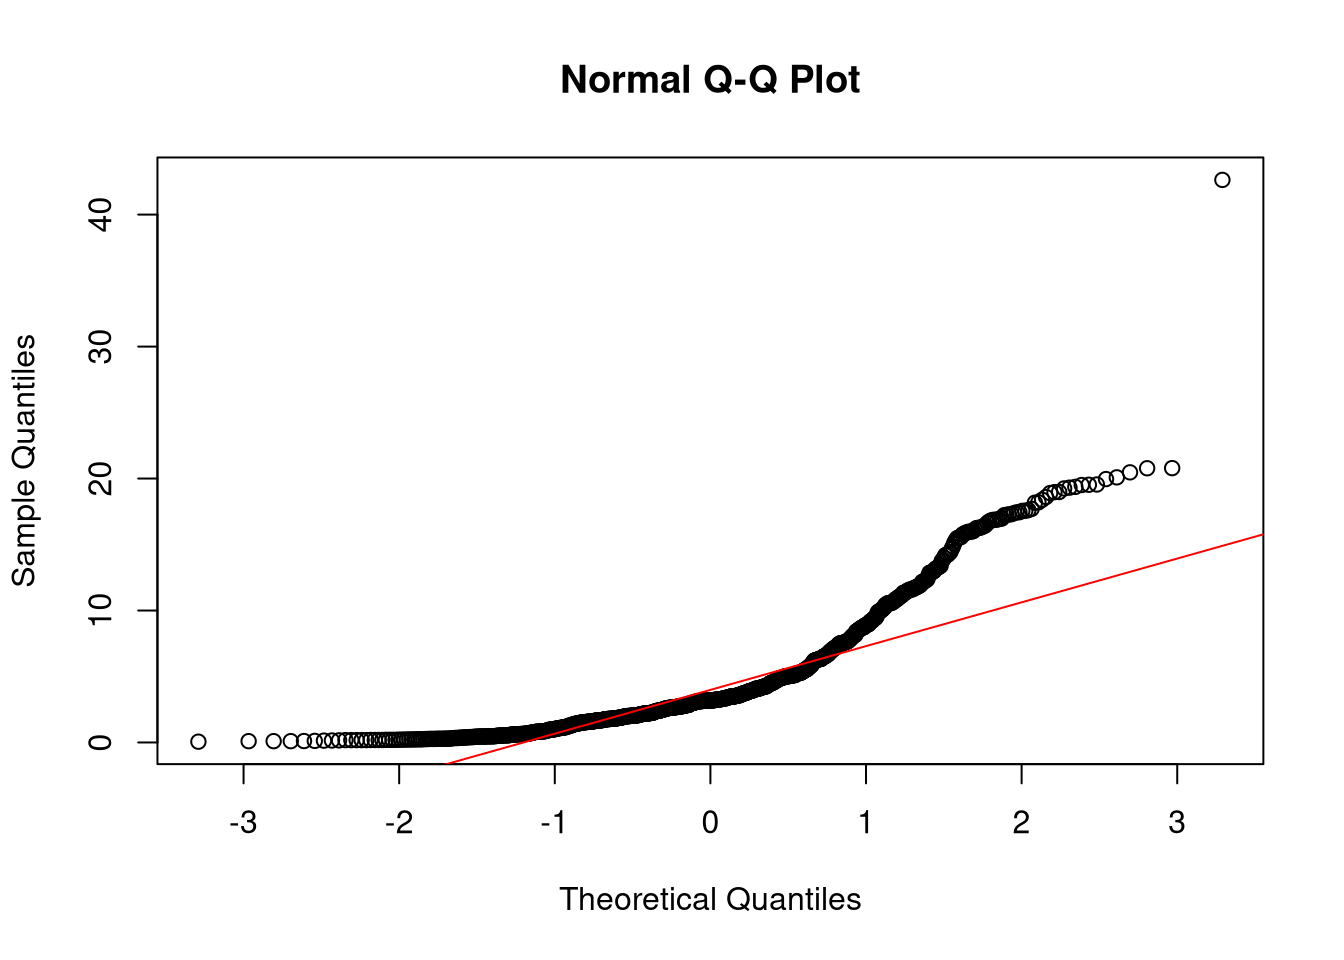
\includegraphics{Practica1_files/figure-latex/unnamed-chunk-26-1.pdf}

\begin{itemize}
\tightlist
\item
  ¿Qué medida de posición considera más apropiada para describir el
  centro de los datos?
\end{itemize}

\begin{Shaded}
\begin{Highlighting}[]
\FunctionTok{hist}\NormalTok{(cpu)}
\FunctionTok{abline}\NormalTok{(}\AttributeTok{v =} \FunctionTok{c}\NormalTok{(}\FunctionTok{mean}\NormalTok{(cpu), }\FunctionTok{median}\NormalTok{(cpu), }\FunctionTok{mean}\NormalTok{(cpu, }\AttributeTok{trim =} \FloatTok{0.1}\NormalTok{)), }\AttributeTok{col =} \FunctionTok{c}\NormalTok{(}\StringTok{"red"}\NormalTok{, }\StringTok{"blue"}\NormalTok{, }\StringTok{"green"}\NormalTok{))}
\FunctionTok{grid}\NormalTok{(}\AttributeTok{nx =} \ConstantTok{NA}\NormalTok{, }\AttributeTok{ny =} \ConstantTok{NULL}\NormalTok{, }\AttributeTok{lty =} \DecValTok{2}\NormalTok{, }\AttributeTok{col =} \StringTok{"gray"}\NormalTok{, }\AttributeTok{lwd =} \DecValTok{1}\NormalTok{)}
\end{Highlighting}
\end{Shaded}

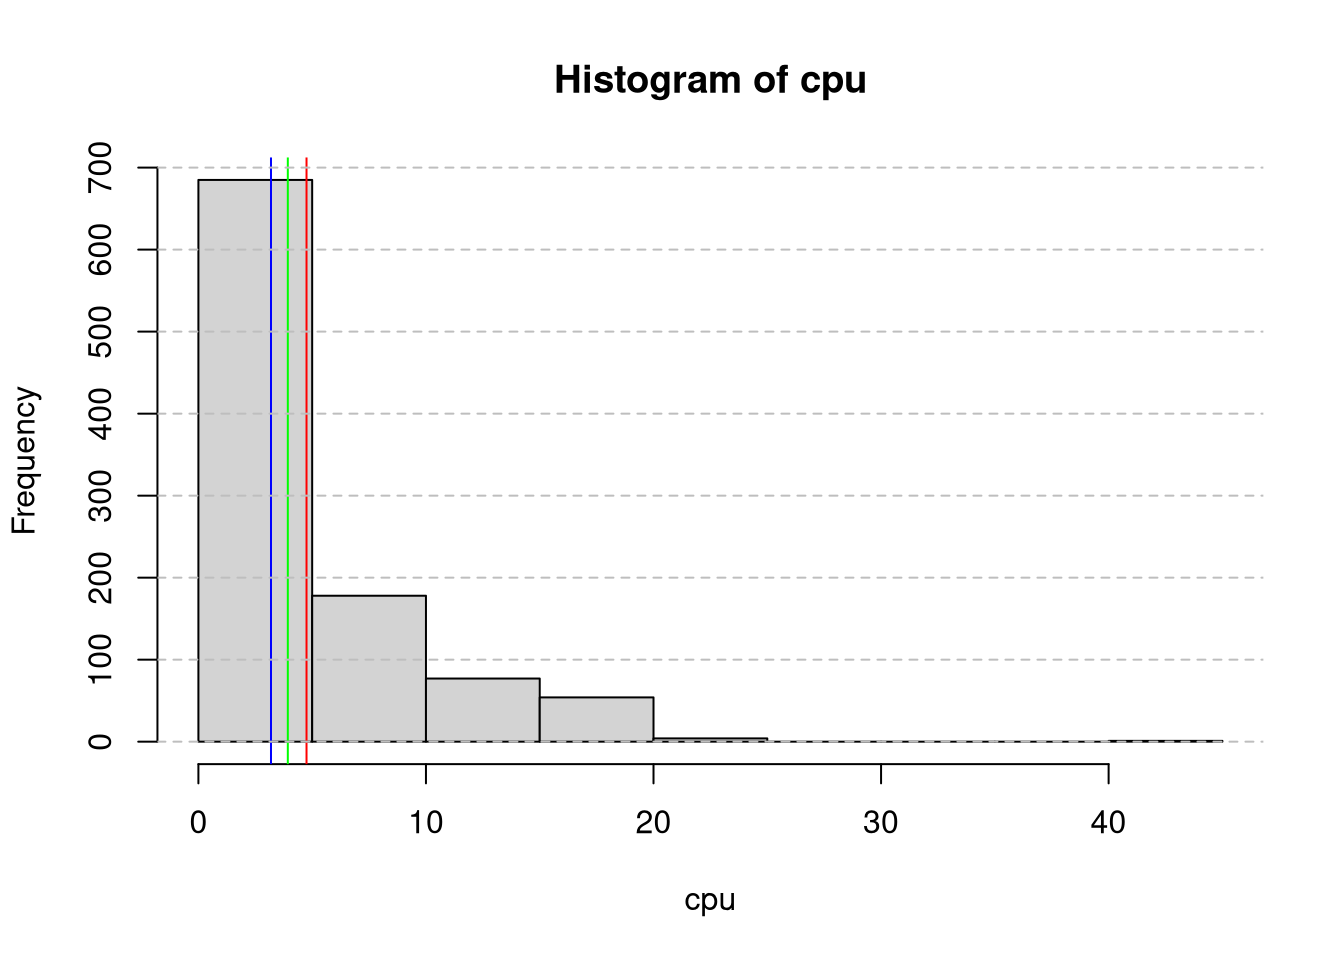
\includegraphics{Practica1_files/figure-latex/unnamed-chunk-27-1.pdf}

\begin{Shaded}
\begin{Highlighting}[]
\FunctionTok{boxplot}\NormalTok{(cpu)}
\FunctionTok{abline}\NormalTok{(}\AttributeTok{h =} \FunctionTok{c}\NormalTok{(}\FunctionTok{mean}\NormalTok{(cpu), }\FunctionTok{median}\NormalTok{(cpu), }\FunctionTok{mean}\NormalTok{(cpu, }\AttributeTok{trim =} \FloatTok{0.1}\NormalTok{)), }\AttributeTok{col =} \FunctionTok{c}\NormalTok{(}\StringTok{"red"}\NormalTok{, }\StringTok{"blue"}\NormalTok{, }\StringTok{"green"}\NormalTok{))}
\end{Highlighting}
\end{Shaded}

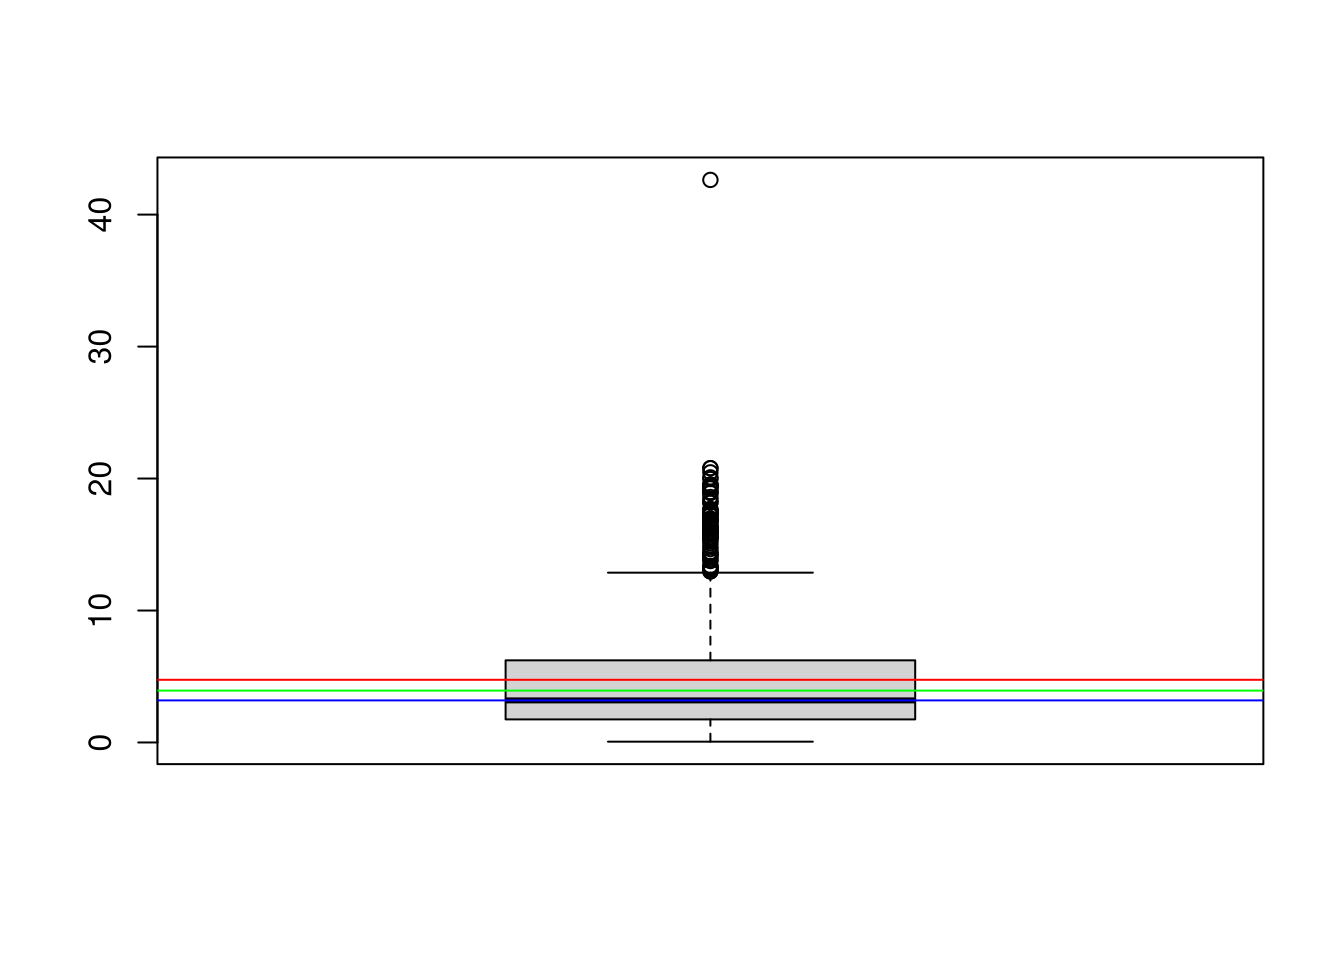
\includegraphics{Practica1_files/figure-latex/unnamed-chunk-27-2.pdf}
****

\hypertarget{ejericio-8}{%
\section{Ejericio 8:}\label{ejericio-8}}

\begin{Shaded}
\begin{Highlighting}[]
\FunctionTok{setwd}\NormalTok{(}\StringTok{"\textasciitilde{}/Documents/FCEyN/Estadistica/Datos"}\NormalTok{)}
\NormalTok{islander\_data }\OtherTok{=} \FunctionTok{read.csv}\NormalTok{(}\StringTok{"Islander\_data.csv"}\NormalTok{)}
\end{Highlighting}
\end{Shaded}

Realizar un histograma con las realizaciones de la variable aleatoria
Diff, la diferencia de tiempos.

\begin{Shaded}
\begin{Highlighting}[]
\FunctionTok{hist}\NormalTok{(islander\_data}\SpecialCharTok{$}\NormalTok{Diff, }\AttributeTok{main =} \StringTok{"Histograma de antes{-}desps del medicamento"}\NormalTok{)}
\end{Highlighting}
\end{Shaded}

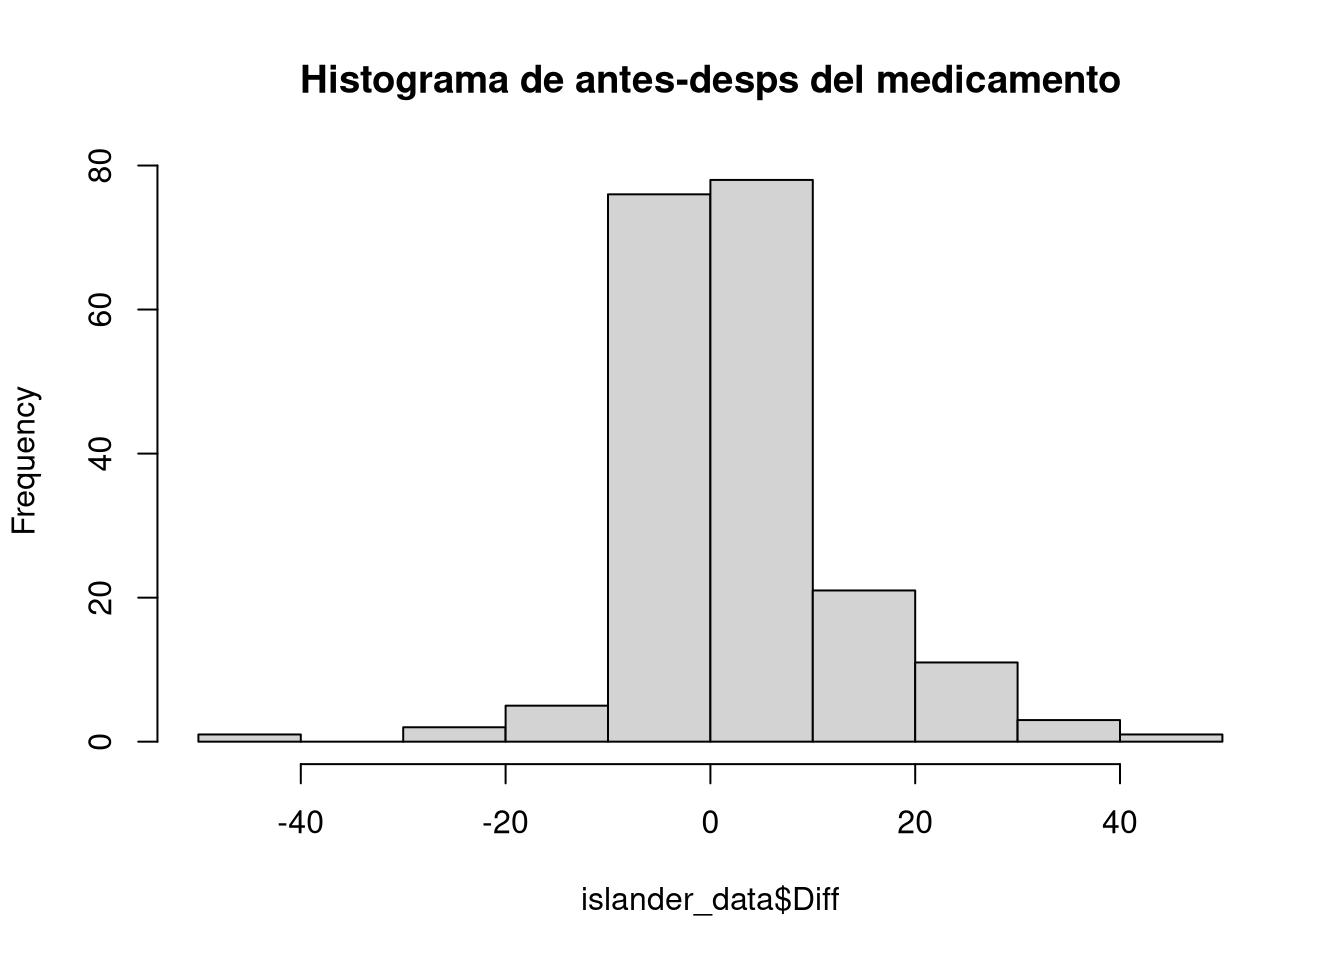
\includegraphics{Practica1_files/figure-latex/unnamed-chunk-29-1.pdf}

\begin{itemize}
\tightlist
\item
  Estimar P(Diff ≤ 1).
\end{itemize}

\begin{Shaded}
\begin{Highlighting}[]
\NormalTok{dif }\OtherTok{=}\NormalTok{ islander\_data}\SpecialCharTok{$}\NormalTok{Diff}
\NormalTok{proba }\OtherTok{=} \DecValTok{0} 
\ControlFlowTok{for}\NormalTok{ (d }\ControlFlowTok{in}\NormalTok{ dif) \{}
  \ControlFlowTok{if}\NormalTok{(d }\SpecialCharTok{\textless{}=} \DecValTok{1}\NormalTok{) proba }\OtherTok{=}\NormalTok{ proba }\SpecialCharTok{+} \DecValTok{1} 
\NormalTok{\}}
\NormalTok{proba }\OtherTok{=}\NormalTok{ proba }\SpecialCharTok{/} \FunctionTok{length}\NormalTok{(dif)}
\NormalTok{proba}
\end{Highlighting}
\end{Shaded}

\begin{verbatim}
## [1] 0.4747475
\end{verbatim}

\begin{itemize}
\tightlist
\item
  Graficar la función de distribución empı́rica de la variable Diff.
\end{itemize}

\begin{Shaded}
\begin{Highlighting}[]
\NormalTok{distrEmpirica }\OtherTok{=} \ControlFlowTok{function}\NormalTok{(V)\{}
\NormalTok{  return }\OtherTok{=} \DecValTok{1}\SpecialCharTok{:}\FunctionTok{length}\NormalTok{(V)}
  \ControlFlowTok{for}\NormalTok{ (i }\ControlFlowTok{in} \DecValTok{1}\SpecialCharTok{:}\FunctionTok{length}\NormalTok{(V)) \{}
\NormalTok{    res }\OtherTok{=} \DecValTok{0}
    \ControlFlowTok{for}\NormalTok{ (d }\ControlFlowTok{in}\NormalTok{ dif) \{}
      \ControlFlowTok{if}\NormalTok{(d }\SpecialCharTok{\textless{}=}\NormalTok{ V[i]) res }\OtherTok{=}\NormalTok{ res }\SpecialCharTok{+} \DecValTok{1}
\NormalTok{    \}}
\NormalTok{    return[i] }\OtherTok{=}\NormalTok{ res }\SpecialCharTok{/} \FunctionTok{length}\NormalTok{(dif)}
\NormalTok{  \}}
  \FunctionTok{return}\NormalTok{(return)}
\NormalTok{\}}
\NormalTok{x }\OtherTok{=} \FunctionTok{seq}\NormalTok{(}\SpecialCharTok{{-}}\DecValTok{41}\NormalTok{,}\DecValTok{50}\NormalTok{,}\FloatTok{0.5}\NormalTok{)}
\FunctionTok{plot}\NormalTok{(x,}\FunctionTok{distrEmpirica}\NormalTok{(x),,}\AttributeTok{xlim =} \FunctionTok{c}\NormalTok{(}\SpecialCharTok{{-}}\DecValTok{41}\NormalTok{,}\DecValTok{50}\NormalTok{),}\AttributeTok{type=}\StringTok{"l"}\NormalTok{)}
\end{Highlighting}
\end{Shaded}

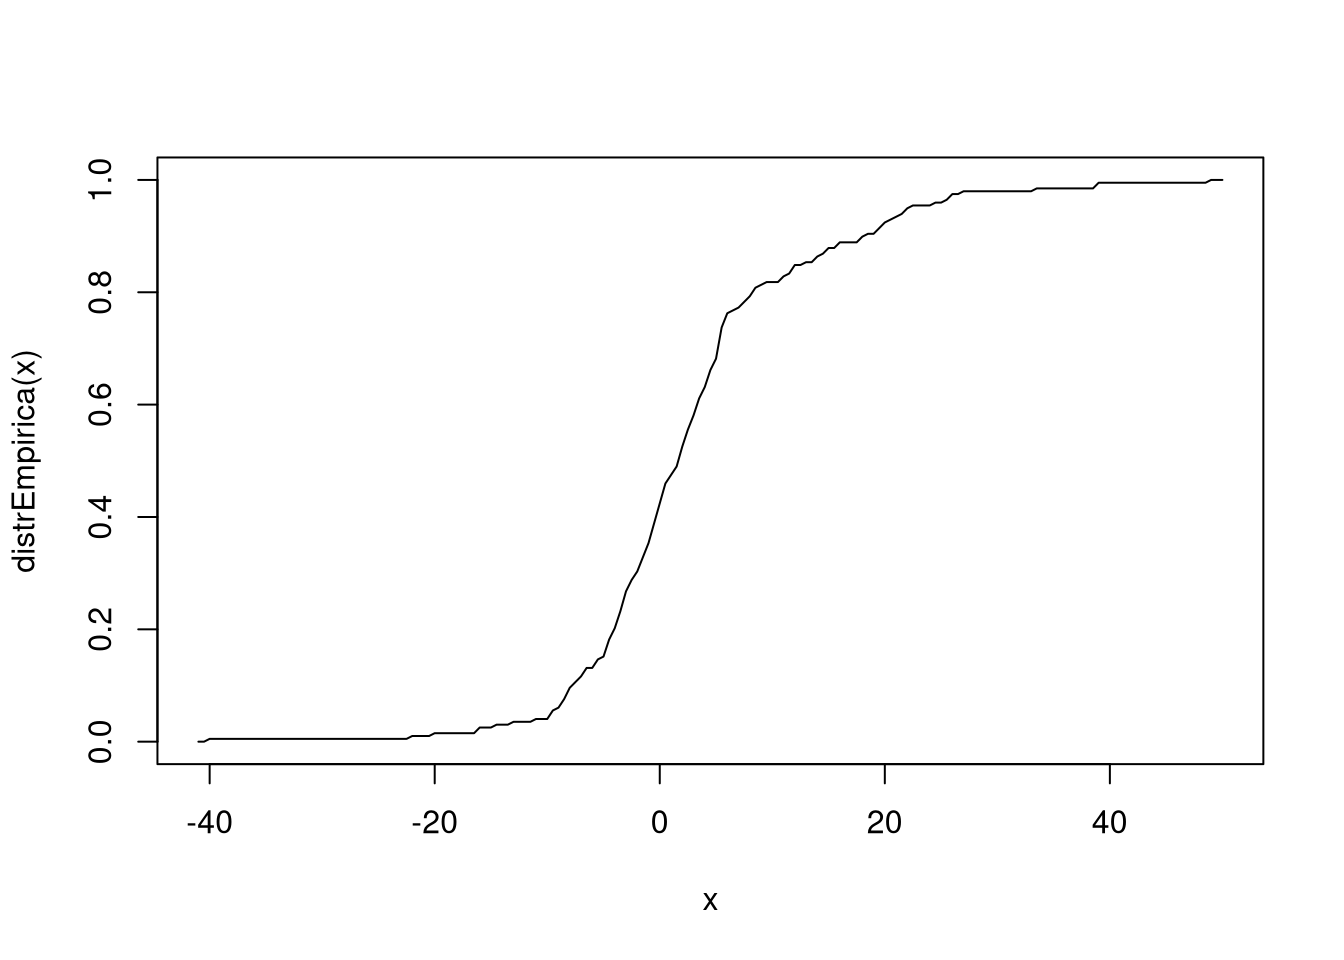
\includegraphics{Practica1_files/figure-latex/unnamed-chunk-31-1.pdf}

\begin{itemize}
\tightlist
\item
  Estimar la densidad de Diff usando estimadores basados en núcleos,
  utilizando diferentes ventanas (h = 0,5, 1,5 y 2,5) y núcleos
  (rectangular, gaussiano y de Epanechnikov). ¿Qué observa?
\end{itemize}

\begin{Shaded}
\begin{Highlighting}[]
\FunctionTok{hist}\NormalTok{(dif, }\AttributeTok{freq =} \ConstantTok{FALSE}\NormalTok{, }\AttributeTok{main =} \StringTok{"Histograma de Diff, ker = rectangular"}\NormalTok{)}
\FunctionTok{lines}\NormalTok{(}\FunctionTok{density}\NormalTok{(dif, }\AttributeTok{kernel =} \StringTok{"rectangular"}\NormalTok{, }\AttributeTok{width =} \FloatTok{0.5}\NormalTok{))}
\end{Highlighting}
\end{Shaded}

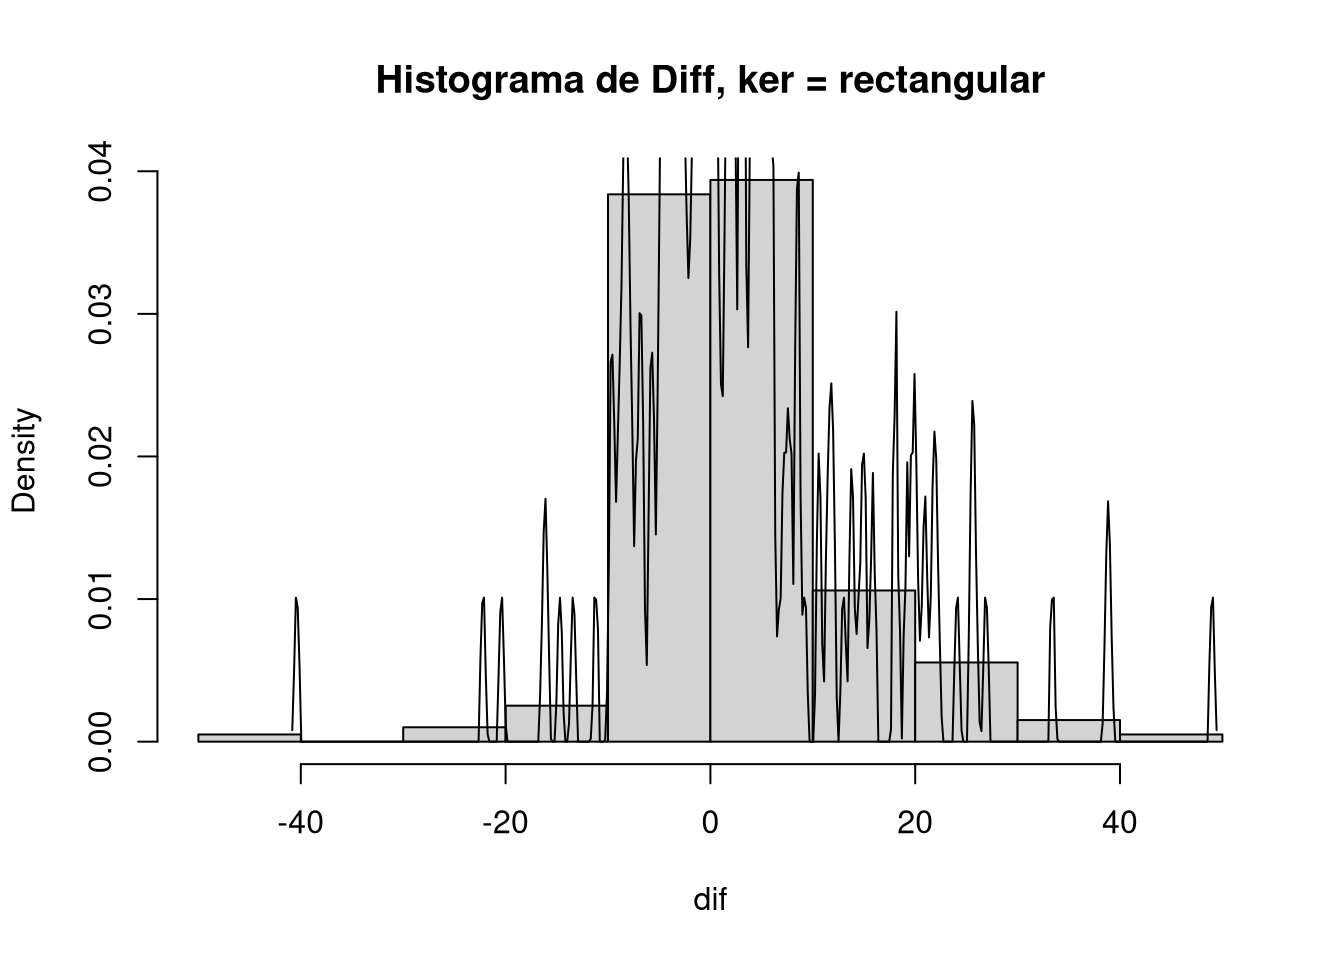
\includegraphics{Practica1_files/figure-latex/unnamed-chunk-32-1.pdf}

\begin{Shaded}
\begin{Highlighting}[]
\FunctionTok{hist}\NormalTok{(dif, }\AttributeTok{freq =} \ConstantTok{FALSE}\NormalTok{, }\AttributeTok{main =} \StringTok{"Histograma de Diff, ker = rectangular"}\NormalTok{)}
\FunctionTok{lines}\NormalTok{(}\FunctionTok{density}\NormalTok{(dif, }\AttributeTok{kernel =} \StringTok{"rectangular"}\NormalTok{, }\AttributeTok{width =} \FloatTok{1.5}\NormalTok{))}
\end{Highlighting}
\end{Shaded}

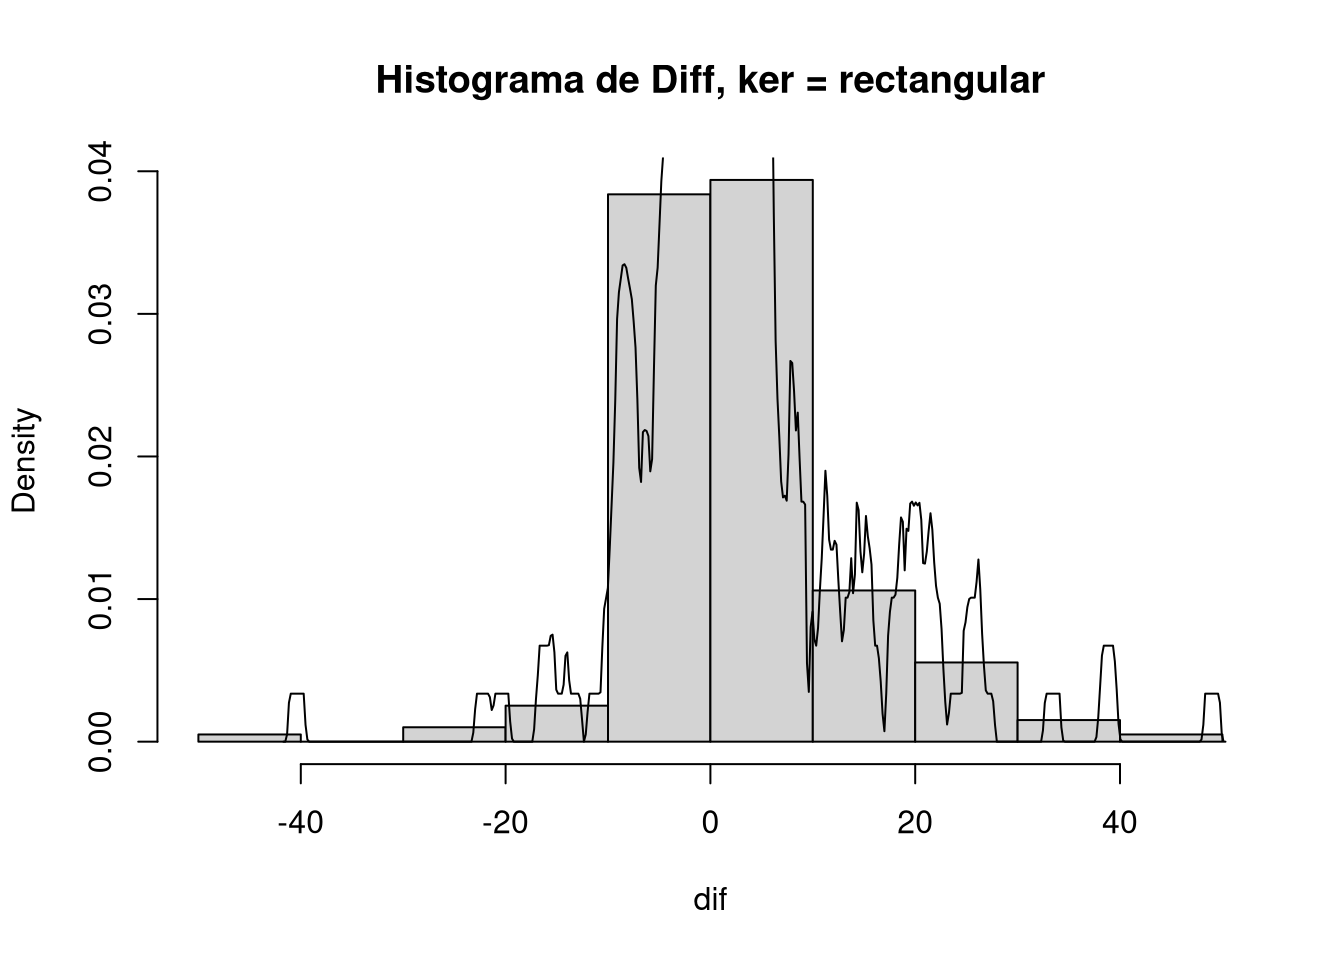
\includegraphics{Practica1_files/figure-latex/unnamed-chunk-32-2.pdf}

\begin{Shaded}
\begin{Highlighting}[]
\FunctionTok{hist}\NormalTok{(dif, }\AttributeTok{freq =} \ConstantTok{FALSE}\NormalTok{, }\AttributeTok{main =} \StringTok{"Histograma de Diff, ker = rectangular"}\NormalTok{)}
\FunctionTok{lines}\NormalTok{(}\FunctionTok{density}\NormalTok{(dif, }\AttributeTok{kernel =} \StringTok{"rectangular"}\NormalTok{, }\AttributeTok{width =} \FloatTok{2.5}\NormalTok{))}
\end{Highlighting}
\end{Shaded}

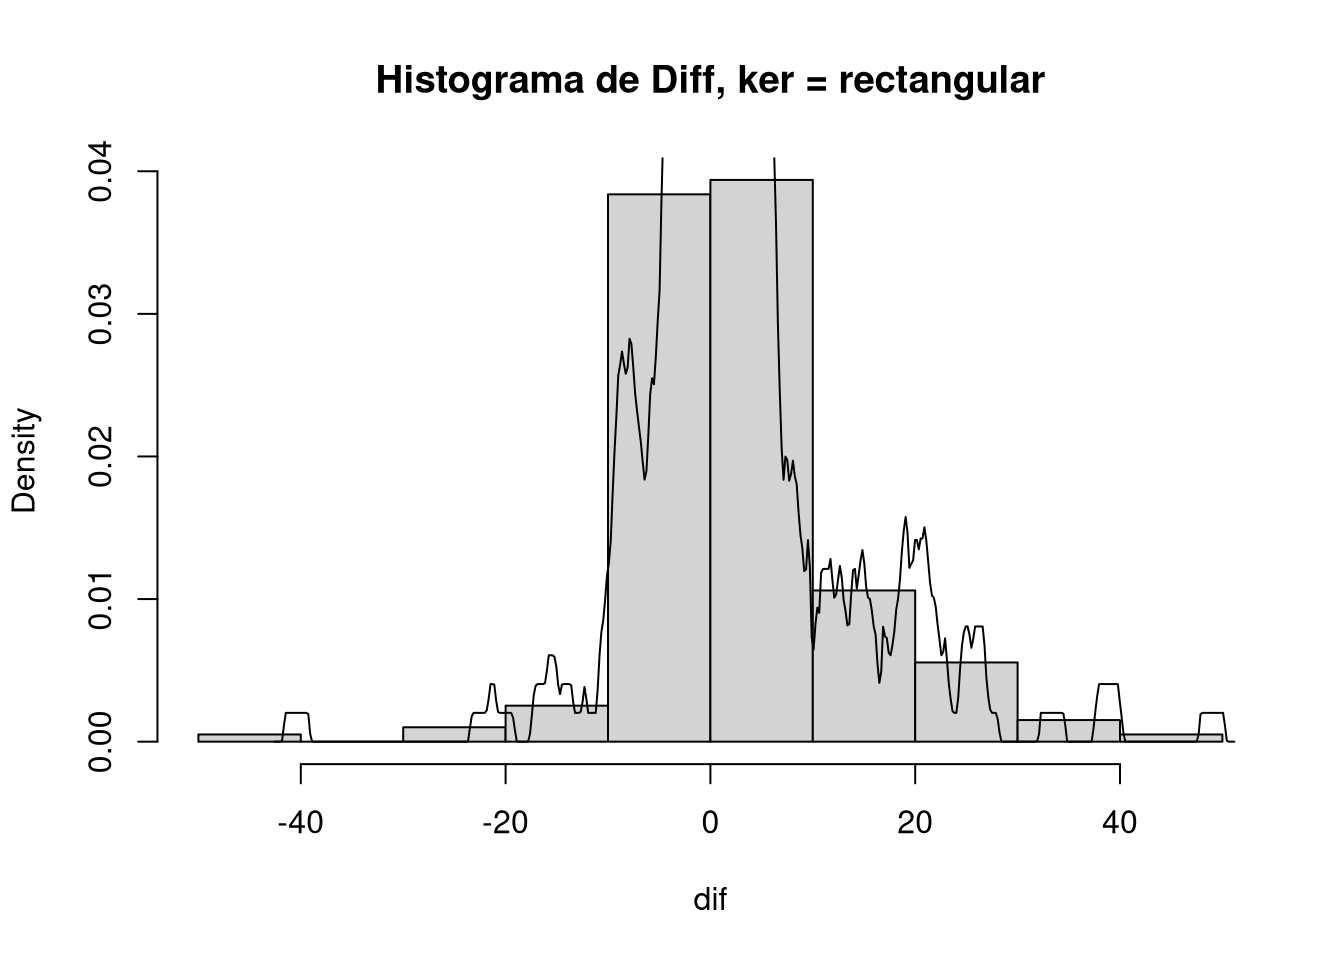
\includegraphics{Practica1_files/figure-latex/unnamed-chunk-32-3.pdf}

\begin{Shaded}
\begin{Highlighting}[]
\FunctionTok{hist}\NormalTok{(dif, }\AttributeTok{freq =} \ConstantTok{FALSE}\NormalTok{, }\AttributeTok{main =} \StringTok{"Histograma de Diff, ker = gauss"}\NormalTok{)}
\FunctionTok{lines}\NormalTok{(}\FunctionTok{density}\NormalTok{(dif, }\AttributeTok{kernel =} \StringTok{"gaussian"}\NormalTok{, }\AttributeTok{width =} \FloatTok{0.5}\NormalTok{))}
\end{Highlighting}
\end{Shaded}

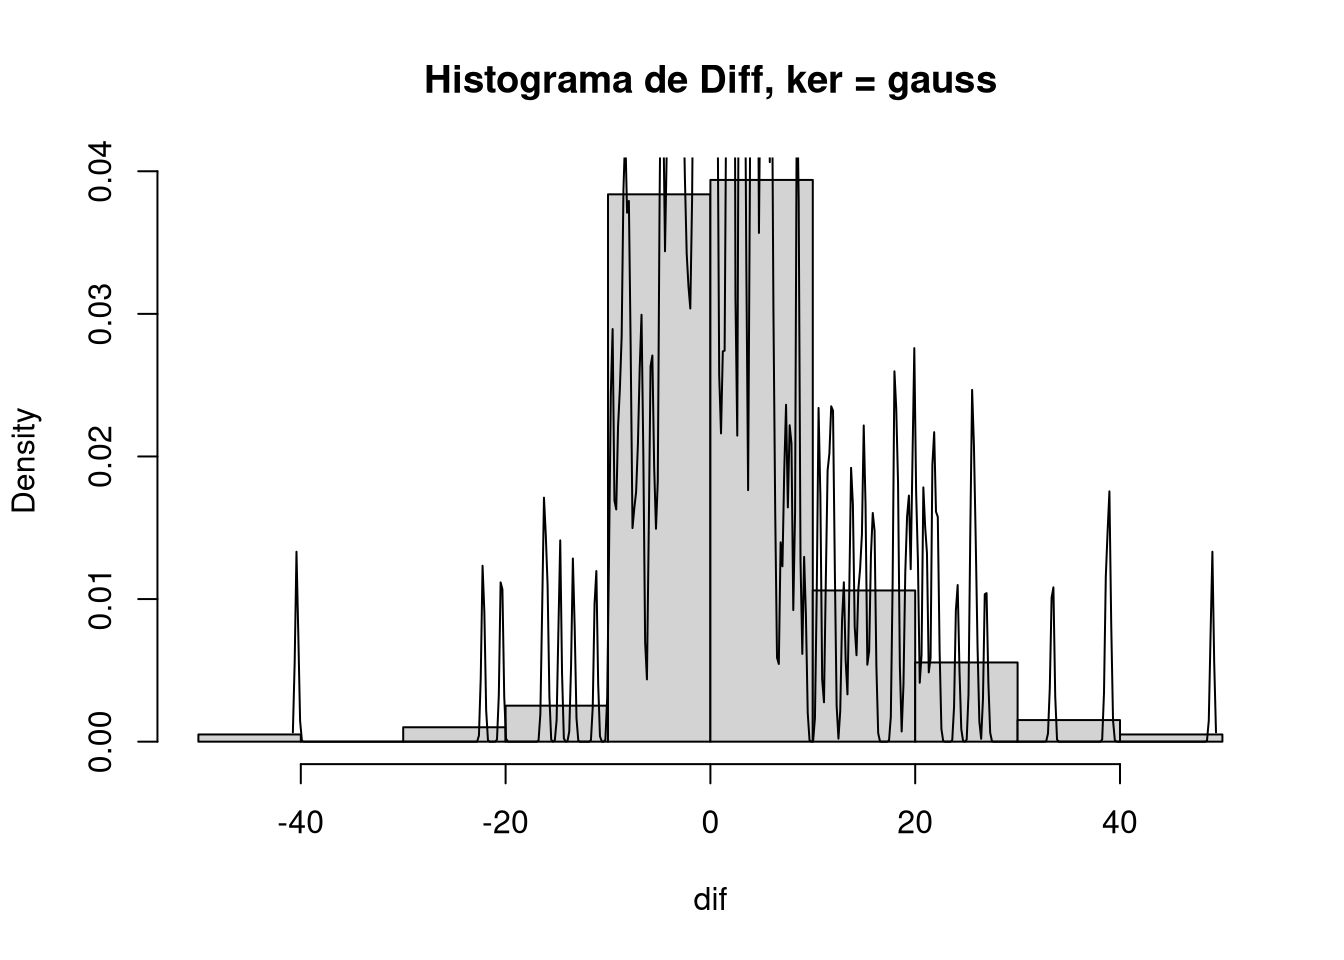
\includegraphics{Practica1_files/figure-latex/unnamed-chunk-32-4.pdf}

\begin{Shaded}
\begin{Highlighting}[]
\FunctionTok{hist}\NormalTok{(dif, }\AttributeTok{freq =} \ConstantTok{FALSE}\NormalTok{, }\AttributeTok{main =} \StringTok{"Histograma de Diff, ker = gauss"}\NormalTok{)}
\FunctionTok{lines}\NormalTok{(}\FunctionTok{density}\NormalTok{(dif, }\AttributeTok{kernel =} \StringTok{"gaussian"}\NormalTok{, }\AttributeTok{width =} \FloatTok{1.5}\NormalTok{))}
\end{Highlighting}
\end{Shaded}

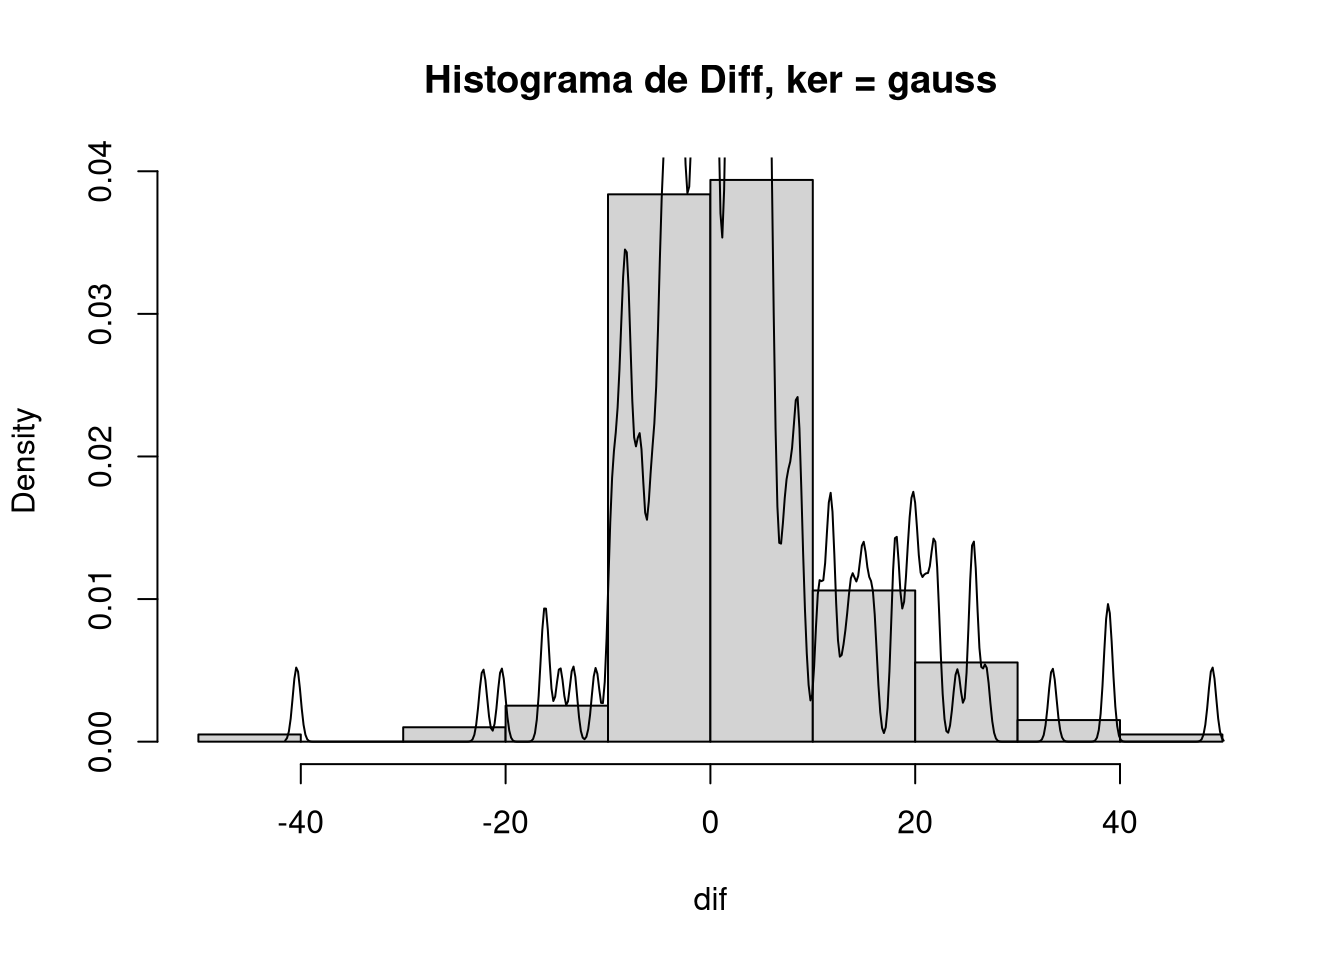
\includegraphics{Practica1_files/figure-latex/unnamed-chunk-32-5.pdf}

\begin{Shaded}
\begin{Highlighting}[]
\FunctionTok{hist}\NormalTok{(dif, }\AttributeTok{freq =} \ConstantTok{FALSE}\NormalTok{, }\AttributeTok{main =} \StringTok{"Histograma de Diff, ker = gauss"}\NormalTok{)}
\FunctionTok{lines}\NormalTok{(}\FunctionTok{density}\NormalTok{(dif, }\AttributeTok{kernel =} \StringTok{"gaussian"}\NormalTok{, }\AttributeTok{width =} \FloatTok{2.5}\NormalTok{))}
\end{Highlighting}
\end{Shaded}

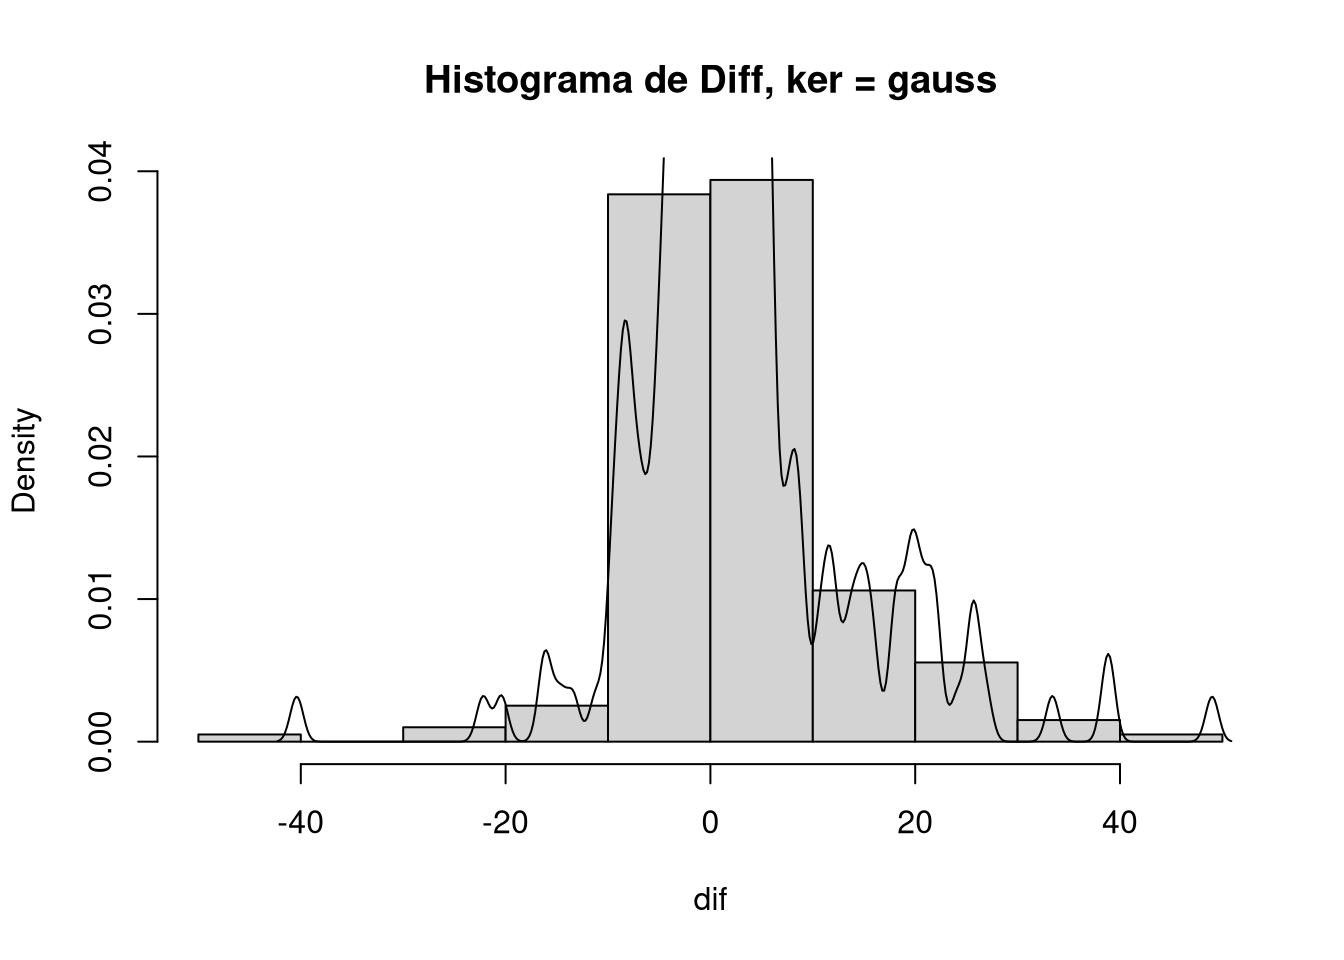
\includegraphics{Practica1_files/figure-latex/unnamed-chunk-32-6.pdf}

\begin{Shaded}
\begin{Highlighting}[]
\FunctionTok{hist}\NormalTok{(dif, }\AttributeTok{freq =} \ConstantTok{FALSE}\NormalTok{, }\AttributeTok{main =} \StringTok{"Histograma de Diff, ker = epanechnikov"}\NormalTok{)}
\FunctionTok{lines}\NormalTok{(}\FunctionTok{density}\NormalTok{(dif, }\AttributeTok{kernel =} \StringTok{"epanechnikov"}\NormalTok{, }\AttributeTok{width =} \FloatTok{0.5}\NormalTok{))}
\end{Highlighting}
\end{Shaded}

\includegraphics{Practica1_files/figure-latex/unnamed-chunk-32-7.pdf}

\begin{Shaded}
\begin{Highlighting}[]
\FunctionTok{hist}\NormalTok{(dif, }\AttributeTok{freq =} \ConstantTok{FALSE}\NormalTok{, }\AttributeTok{main =} \StringTok{"Histograma de Diff, ker = epanechnikov"}\NormalTok{)}
\FunctionTok{lines}\NormalTok{(}\FunctionTok{density}\NormalTok{(dif, }\AttributeTok{kernel =} \StringTok{"epanechnikov"}\NormalTok{, }\AttributeTok{width =} \FloatTok{1.5}\NormalTok{))}
\end{Highlighting}
\end{Shaded}

\includegraphics{Practica1_files/figure-latex/unnamed-chunk-32-8.pdf}

\begin{Shaded}
\begin{Highlighting}[]
\FunctionTok{hist}\NormalTok{(dif, }\AttributeTok{freq =} \ConstantTok{FALSE}\NormalTok{, }\AttributeTok{main =} \StringTok{"Histograma de Diff, ker = epanechnikov"}\NormalTok{)}
\FunctionTok{lines}\NormalTok{(}\FunctionTok{density}\NormalTok{(dif, }\AttributeTok{kernel =} \StringTok{"epanechnikov"}\NormalTok{, }\AttributeTok{width =} \FloatTok{2.5}\NormalTok{))}
\end{Highlighting}
\end{Shaded}

\includegraphics{Practica1_files/figure-latex/unnamed-chunk-32-9.pdf}
****

\hypertarget{ejericio-9-con-los-datos-de-debernardi.csv}{%
\section{Ejericio 9: (con los datos de
Debernardi.csv)}\label{ejericio-9-con-los-datos-de-debernardi.csv}}

\begin{itemize}
\tightlist
\item
  Realizar histogramas para la variable LYVE1 basados en los datos
  brindados para las observaciones que cumplen diagnosis=1, diagnosis=2
  y diagnosis=3. Es decir efectuar histogramas según los niveles de la
  variable factor diagnosis. Indicar las caracterı́sticas más
  sobresalientes de los histogramas y aquellas que los diferencian.
  \textgreater{} Las densidades empiricas condicionando a diagnosis 1 y
  2 parecen ser muy parecidas, en cambio la de 3, aparanta tener mas
  cantidad de datos en la moda.
\end{itemize}

\begin{Shaded}
\begin{Highlighting}[]
\NormalTok{ly\_diag1 }\OtherTok{=}\NormalTok{ debD}\SpecialCharTok{$}\NormalTok{LYVE1[ debD}\SpecialCharTok{$}\NormalTok{diagnosis }\SpecialCharTok{==} \DecValTok{1}\NormalTok{ ]}
\NormalTok{ly\_diag2 }\OtherTok{=}\NormalTok{ debD}\SpecialCharTok{$}\NormalTok{LYVE1[ debD}\SpecialCharTok{$}\NormalTok{diagnosis }\SpecialCharTok{==} \DecValTok{2}\NormalTok{ ]}
\NormalTok{ly\_diag3 }\OtherTok{=}\NormalTok{ debD}\SpecialCharTok{$}\NormalTok{LYVE1[ debD}\SpecialCharTok{$}\NormalTok{diagnosis }\SpecialCharTok{==} \DecValTok{3}\NormalTok{ ]}
\FunctionTok{hist}\NormalTok{(ly\_diag1, }\AttributeTok{main =} \StringTok{"Histograma de LYVE1 condicionado a diagnosis 1"}\NormalTok{)}
\end{Highlighting}
\end{Shaded}

\includegraphics{Practica1_files/figure-latex/unnamed-chunk-33-1.pdf}

\begin{Shaded}
\begin{Highlighting}[]
\FunctionTok{hist}\NormalTok{(ly\_diag2, }\AttributeTok{main =} \StringTok{"Histograma de LYVE1 condicionado a diagnosis 2"}\NormalTok{)}
\end{Highlighting}
\end{Shaded}

\includegraphics{Practica1_files/figure-latex/unnamed-chunk-33-2.pdf}

\begin{Shaded}
\begin{Highlighting}[]
\FunctionTok{hist}\NormalTok{(ly\_diag3, }\AttributeTok{main =} \StringTok{"Histograma de LYVE1 condicionado a diagnosis 3"}\NormalTok{)}
\end{Highlighting}
\end{Shaded}

\includegraphics{Practica1_files/figure-latex/unnamed-chunk-33-3.pdf}

\begin{itemize}
\tightlist
\item
  Graficar, en distintos colores y superpuestas, las funciones de
  distribución empı́ricas de la variable LYVE1 según los niveles de la
  variable factor diagnosis. Decidir si la siguiente afirmación es
  verdadera o falsa y justificar: ``los valores de la variable LYVE1
  tienden a ser más altos entre quienes tienen cáncer de páncreas que
  entre quienes sufren otras enfermedades asociadas al páncreas''
  \textgreater{} La afirmacion parece ser verdadera ya que para LY..
  diagnosis == 3, tiende a crecer de forma mas rapida en los datos mas
  ``altos''.
\end{itemize}

\begin{Shaded}
\begin{Highlighting}[]
\NormalTok{ly\_diag1}
\end{Highlighting}
\end{Shaded}

\begin{verbatim}
##   [1] 0.893219200 2.037585000 0.145588900 0.002804880 0.000859560 0.003393000
##   [7] 0.174380800 0.003573960 0.001945320 0.278778500 0.001176240 0.860336800
##  [13] 1.416314000 1.516773000 0.599644900 0.002035800 0.001673880 0.003212040
##  [19] 2.285351000 0.583009700 0.004976400 0.003800160 0.653984400 0.583009700
##  [25] 2.440180000 1.044411000 0.748617200 2.392864000 0.000995280 1.600313000
##  [31] 0.002895360 5.309197000 4.239308000 0.000542880 1.008584000 6.925281000
##  [37] 0.000633360 0.001357200 1.013824000 0.963804000 4.090239000 0.462653000
##  [43] 7.300192000 6.836843000 0.000271440 0.110310600 0.008919911 0.062164210
##  [49] 0.007113679 0.019425770 0.012780680 0.001719120 0.001311960 0.008404655
##  [55] 0.001682586 0.013293490 1.464090000 0.048931690 0.000647148 0.007113679
##  [61] 0.000814320 0.001266720 0.004787650 0.017642170 0.000647148 0.000904800
##  [67] 0.000678600 3.816866000 0.028980820 0.001492920 0.000497640 0.000906008
##  [73] 0.008662283 0.010465680 0.000388289 0.002976883 0.000906008 0.005046098
##  [79] 4.980546000 0.005304546 0.003494602 0.000129430 0.003753461 0.016368170
##  [85] 0.000647148 0.023728300 0.000129430 0.007113679 0.003076320 1.994221000
##  [91] 0.000129430 0.001221480 0.004524000 0.001990560 3.173585000 0.091370200
##  [97] 1.858508000 1.344993000 0.279427000 0.002533440 4.242341000 0.022322830
## [103] 0.571180600 0.011928710 8.160930000 3.954307000 0.924147900 0.864247600
## [109] 0.011928710 2.101149000 0.535693200 0.001402440 2.776768000 0.001854840
## [115] 4.855595000 1.560655000 3.629087000 0.002850120 4.214547000 0.000542880
## [121] 0.086186990 5.728702000 0.005835960 4.637318000 0.999371300 2.101149000
## [127] 1.056174000 5.113560000 1.079988000 0.594000100 2.357376000 2.984651000
## [133] 4.616530000 7.069545000 1.434706000 3.909729000 8.223294000 3.658579000
## [139] 0.464718600 0.138721100 2.795054000 2.423368000 0.001131000 0.115870000
## [145] 4.512589000 0.002307240 1.228042000 3.268218000 2.049820000 8.319249000
## [151] 0.487718200 5.953427000 3.043465000 1.600313000 0.656364900 0.901411000
## [157] 0.001311960 1.174235000 0.157614900 0.406950700 1.642057000 1.632705000
## [163] 1.155294000 0.874513000 0.000814320 0.512019000 0.001900080 0.151870000
## [169] 0.406950700 0.697202800 0.000814320 0.000316680 2.582407000 0.109682000
## [175] 0.000316680 0.000588120 0.000904800 0.131196600 0.001357200 0.228900000
## [181] 0.003483480 0.109682600 0.002262000
\end{verbatim}

\begin{Shaded}
\begin{Highlighting}[]
\NormalTok{disEmp1 }\OtherTok{=} \ControlFlowTok{function}\NormalTok{(V)\{}
\NormalTok{  return }\OtherTok{=} \DecValTok{1}\SpecialCharTok{:}\FunctionTok{length}\NormalTok{(V)}
  \ControlFlowTok{for}\NormalTok{ (i }\ControlFlowTok{in} \DecValTok{1}\SpecialCharTok{:}\FunctionTok{length}\NormalTok{(V)) \{}
\NormalTok{    res }\OtherTok{=} \DecValTok{0}
    \ControlFlowTok{for}\NormalTok{ (d }\ControlFlowTok{in}\NormalTok{ ly\_diag1) \{}
      \ControlFlowTok{if}\NormalTok{(d }\SpecialCharTok{\textless{}=}\NormalTok{ V[i]) res }\OtherTok{=}\NormalTok{ res }\SpecialCharTok{+} \DecValTok{1}
\NormalTok{    \}}
\NormalTok{    return[i] }\OtherTok{=}\NormalTok{ res }\SpecialCharTok{/} \FunctionTok{length}\NormalTok{(ly\_diag1)}
\NormalTok{  \}}
  \FunctionTok{return}\NormalTok{(return)}
\NormalTok{\}}
\NormalTok{disEmp2 }\OtherTok{=} \ControlFlowTok{function}\NormalTok{(V)\{}
\NormalTok{  return }\OtherTok{=} \DecValTok{1}\SpecialCharTok{:}\FunctionTok{length}\NormalTok{(V)}
  \ControlFlowTok{for}\NormalTok{ (i }\ControlFlowTok{in} \DecValTok{1}\SpecialCharTok{:}\FunctionTok{length}\NormalTok{(V)) \{}
\NormalTok{    res }\OtherTok{=} \DecValTok{0}
    \ControlFlowTok{for}\NormalTok{ (d }\ControlFlowTok{in}\NormalTok{ ly\_diag2) \{}
      \ControlFlowTok{if}\NormalTok{(d }\SpecialCharTok{\textless{}=}\NormalTok{ V[i]) res }\OtherTok{=}\NormalTok{ res }\SpecialCharTok{+} \DecValTok{1}
\NormalTok{    \}}
\NormalTok{    return[i] }\OtherTok{=}\NormalTok{ res }\SpecialCharTok{/} \FunctionTok{length}\NormalTok{(ly\_diag2)}
\NormalTok{  \}}
  \FunctionTok{return}\NormalTok{(return)}
\NormalTok{\}}
\NormalTok{disEmp3 }\OtherTok{=} \ControlFlowTok{function}\NormalTok{(V)\{}
\NormalTok{  return }\OtherTok{=} \DecValTok{1}\SpecialCharTok{:}\FunctionTok{length}\NormalTok{(V)}
  \ControlFlowTok{for}\NormalTok{ (i }\ControlFlowTok{in} \DecValTok{1}\SpecialCharTok{:}\FunctionTok{length}\NormalTok{(V)) \{}
\NormalTok{    res }\OtherTok{=} \DecValTok{0}
    \ControlFlowTok{for}\NormalTok{ (d }\ControlFlowTok{in}\NormalTok{ ly\_diag3) \{}
      \ControlFlowTok{if}\NormalTok{(d }\SpecialCharTok{\textless{}=}\NormalTok{ V[i]) res }\OtherTok{=}\NormalTok{ res }\SpecialCharTok{+} \DecValTok{1}
\NormalTok{    \}}
\NormalTok{    return[i] }\OtherTok{=}\NormalTok{ res }\SpecialCharTok{/} \FunctionTok{length}\NormalTok{(ly\_diag3)}
\NormalTok{  \}}
  \FunctionTok{return}\NormalTok{(return)}
\NormalTok{\}}
\NormalTok{y }\OtherTok{=} \FunctionTok{seq}\NormalTok{(}\DecValTok{0}\NormalTok{,}\DecValTok{24}\NormalTok{,}\FloatTok{0.01}\NormalTok{)}

\FunctionTok{plot}\NormalTok{(y,}\FunctionTok{disEmp1}\NormalTok{(y),}\AttributeTok{type =} \StringTok{"l"}\NormalTok{, }\AttributeTok{col =} \StringTok{"red"}\NormalTok{, }\AttributeTok{xlab =} \StringTok{"x"}\NormalTok{, }\AttributeTok{main =} \StringTok{"Funciones de distribuciones empiricas"}\NormalTok{)}
\FunctionTok{lines}\NormalTok{(y,}\FunctionTok{disEmp2}\NormalTok{(y),}\AttributeTok{col =} \StringTok{"blue"}\NormalTok{)}
\FunctionTok{lines}\NormalTok{(y,}\FunctionTok{disEmp3}\NormalTok{(y),}\AttributeTok{col =} \StringTok{"green"}\NormalTok{)}
\end{Highlighting}
\end{Shaded}

\includegraphics{Practica1_files/figure-latex/unnamed-chunk-34-1.pdf}

\begin{itemize}
\tightlist
\item
  Realizar boxplots paralelos para la variable LYVE1 según los niveles
  de la variable factor diagnosis, considerando el sexo de los pacientes
  (variable sex). Decidir si la siguiente afirmación es verdadera o
  falsa y justificar: ``en términos generales, el sexo del paciente no
  afecta los niveles de la proteı́na que se mide en la variable LYVE1''.
  \textgreater{} Por lo menos para valores de Ly.. condicionando a
  diagnosis = 1, parece tener una leve inclinacion a hombres respecto a
  mujeres.
\end{itemize}

\begin{Shaded}
\begin{Highlighting}[]
\NormalTok{ly\_diag1\_M }\OtherTok{=}\NormalTok{ debD}\SpecialCharTok{$}\NormalTok{LYVE1[debD}\SpecialCharTok{$}\NormalTok{sex }\SpecialCharTok{==} \StringTok{"M"} \SpecialCharTok{\&}\NormalTok{ debD}\SpecialCharTok{$}\NormalTok{diagnosis }\SpecialCharTok{==} \DecValTok{1}\NormalTok{]}
\NormalTok{ly\_diag1\_F }\OtherTok{=}\NormalTok{ debD}\SpecialCharTok{$}\NormalTok{LYVE1[debD}\SpecialCharTok{$}\NormalTok{sex }\SpecialCharTok{==} \StringTok{"F"} \SpecialCharTok{\&}\NormalTok{ debD}\SpecialCharTok{$}\NormalTok{diagnosis }\SpecialCharTok{==} \DecValTok{1}\NormalTok{]}
\NormalTok{ly\_diag2\_M }\OtherTok{=}\NormalTok{ debD}\SpecialCharTok{$}\NormalTok{LYVE1[debD}\SpecialCharTok{$}\NormalTok{sex }\SpecialCharTok{==} \StringTok{"M"} \SpecialCharTok{\&}\NormalTok{ debD}\SpecialCharTok{$}\NormalTok{diagnosis }\SpecialCharTok{==} \DecValTok{2}\NormalTok{]}
\NormalTok{ly\_diag2\_F }\OtherTok{=}\NormalTok{ debD}\SpecialCharTok{$}\NormalTok{LYVE1[debD}\SpecialCharTok{$}\NormalTok{sex }\SpecialCharTok{==} \StringTok{"F"} \SpecialCharTok{\&}\NormalTok{ debD}\SpecialCharTok{$}\NormalTok{diagnosis }\SpecialCharTok{==} \DecValTok{2}\NormalTok{]}
\NormalTok{ly\_diag3\_M }\OtherTok{=}\NormalTok{ debD}\SpecialCharTok{$}\NormalTok{LYVE1[debD}\SpecialCharTok{$}\NormalTok{sex }\SpecialCharTok{==} \StringTok{"M"} \SpecialCharTok{\&}\NormalTok{ debD}\SpecialCharTok{$}\NormalTok{diagnosis }\SpecialCharTok{==} \DecValTok{3}\NormalTok{]}
\NormalTok{ly\_diag3\_F }\OtherTok{=}\NormalTok{ debD}\SpecialCharTok{$}\NormalTok{LYVE1[debD}\SpecialCharTok{$}\NormalTok{sex }\SpecialCharTok{==} \StringTok{"F"} \SpecialCharTok{\&}\NormalTok{ debD}\SpecialCharTok{$}\NormalTok{diagnosis }\SpecialCharTok{==} \DecValTok{3}\NormalTok{]}
\FunctionTok{boxplot}\NormalTok{(ly\_diag1\_M,ly\_diag1\_F, }\AttributeTok{main =} \StringTok{"ly.. diagnosis1, M y F"}\NormalTok{)}
\end{Highlighting}
\end{Shaded}

\includegraphics{Practica1_files/figure-latex/unnamed-chunk-35-1.pdf}

\begin{Shaded}
\begin{Highlighting}[]
\FunctionTok{boxplot}\NormalTok{(ly\_diag2\_M,ly\_diag2\_F, }\AttributeTok{main =} \StringTok{"ly.. diagnosis2, M y F"}\NormalTok{)}
\end{Highlighting}
\end{Shaded}

\includegraphics{Practica1_files/figure-latex/unnamed-chunk-35-2.pdf}

\begin{Shaded}
\begin{Highlighting}[]
\FunctionTok{boxplot}\NormalTok{(ly\_diag3\_M,ly\_diag3\_F, }\AttributeTok{main =} \StringTok{"ly.. diagnosis3, M y F"}\NormalTok{)}
\end{Highlighting}
\end{Shaded}

\includegraphics{Practica1_files/figure-latex/unnamed-chunk-35-3.pdf}

\begin{itemize}
\tightlist
\item
  Graficar superpuestas las densidades estimadas, que brinda la función
  density, para la variable LYVE1 según los niveles de la variable
  factor diagnosis. Describir las caracterı́sticas más sobresalientes de
  las densidades estimadas y aquellas que las diferencian.
  \textgreater{} La caracteristica mas notoria que veo es la misma
  caracteristica que en la funcion de proba acumulada.
\end{itemize}

\begin{Shaded}
\begin{Highlighting}[]
\FunctionTok{plot}\NormalTok{(}\FunctionTok{density}\NormalTok{(ly\_diag1),}\AttributeTok{col =} \StringTok{"red"}\NormalTok{, }\AttributeTok{main =} \StringTok{"Densidades de las Ly... diagnosis 1 2 y 3"}\NormalTok{, }\AttributeTok{xlab =} \StringTok{"x"}\NormalTok{)}
\FunctionTok{lines}\NormalTok{(}\FunctionTok{density}\NormalTok{(ly\_diag2), }\AttributeTok{col =} \StringTok{"blue"}\NormalTok{)}
\FunctionTok{lines}\NormalTok{(}\FunctionTok{density}\NormalTok{(ly\_diag3), }\AttributeTok{col =} \StringTok{"green"}\NormalTok{)}
\end{Highlighting}
\end{Shaded}

\includegraphics{Practica1_files/figure-latex/unnamed-chunk-36-1.pdf}

\end{document}
